


%% Select the dissertation mode on
% See the documentation for more information about the available class options
% If you give option 'draft' or 'draft*', the draft mode is set on
\documentclass[dissertation,nocontribution,draft*]{aaltoseries}
\usepackage[utf8]{inputenc}
% Lipsum package generates bullshit
\usepackage{lipsum}
% Set the document languages
\usepackage[finnish,swedish,english]{babel}

% For figures
%\usepackage{epsfig} % less modern
\usepackage{subfigure} 
\usepackage{array} 

% For citations
\usepackage{natbib}
\bibpunct{(}{)}{;}{a}{,}{,}

% For algorithms
\usepackage{algorithm}
\usepackage{algorithmic}

\usepackage{times,amsmath} % Add all your packages here
\usepackage{stfloats}
\usepackage{multirow}
\usepackage{rotating}
\usepackage{amssymb}
\usepackage{amsmath}
%\usepackage{paralist}
\usepackage{subfigure} 
\usepackage{floatflt}
\usepackage{wrapfig}

%\usepackage{auto-pst-pdf}
\usepackage[off]{auto-pst-pdf}
\usepackage{graphicx} % more modern
\usepackage{psfrag}

\usepackage{nomencl}
\makenomenclature

\newcommand{\bmx}[0]{\begin{bmatrix}}
\newcommand{\emx}[0]{\end{bmatrix}}
\newcommand{\qt}[1]{\left<#1\right>}
\newcommand{\qexp}[1]{\left<#1\right>}
\newcommand{\qlay}[1]{\left[#1\right]}
\newcommand{\vect}[1]{\mathbf{#1}}
\newcommand{\vects}[1]{\boldsymbol{#1}}
\newcommand{\matr}[1]{\mathbf{#1}}
\newcommand{\var}[0]{\operatorname{Var}}
\newcommand{\cov}[0]{\operatorname{Cov}}
\newcommand{\diag}[0]{\operatorname{diag}}
\newcommand{\matrs}[1]{\boldsymbol{#1}}
\newcommand{\va}[0]{\vect{a}}
\newcommand{\vb}[0]{\vect{b}}
\newcommand{\vc}[0]{\vect{c}}
\newcommand{\vh}[0]{\vect{h}}
\newcommand{\vv}[0]{\vect{v}}
\newcommand{\vf}[0]{\vect{f}}
\newcommand{\vx}[0]{\vect{x}}
\newcommand{\vy}[0]{\vect{y}}
\newcommand{\vg}[0]{\vect{g}}
\newcommand{\vr}[0]{\vect{r}}
\newcommand{\vq}[0]{\vect{q}}
\newcommand{\vm}[0]{\vect{m}}
\newcommand{\vs}[0]{\vect{s}}
\newcommand{\vw}[0]{\vect{w}}
\newcommand{\vL}[0]{\vect{L}}
\newcommand{\vp}[0]{\vect{p}}
\newcommand{\mW}[0]{\matr{W}}
\newcommand{\mG}[0]{\matr{G}}
\newcommand{\mX}[0]{\matr{X}}
\newcommand{\mY}[0]{\matr{Y}}
\newcommand{\mK}[0]{\matr{K}}
\newcommand{\mH}[0]{\matr{H}}
\newcommand{\mQ}[0]{\matr{Q}}
\newcommand{\mU}[0]{\matr{U}}
\newcommand{\mR}[0]{\matr{R}}
\newcommand{\mV}[0]{\matr{V}}
\newcommand{\mA}{\matr{A}}
\newcommand{\mD}{\matr{D}}
\newcommand{\mC}{\matr{C}}
\newcommand{\mS}{\matr{S}}
\newcommand{\mI}{\matr{I}}
\newcommand{\mL}{\matr{L}}
\newcommand{\mzero}[0]{\matr{0}}
\newcommand{\td}[0]{\text{d}}
\newcommand{\valpha}[0]{\vects{\alpha}}
\newcommand{\vbeta}[0]{\vects{\beta}}
\newcommand{\vsig}[0]{\vects{\sigma}}
\newcommand{\vmu}[0]{\vects{\mu}}
\newcommand{\vone}[0]{\vects{1}}
\newcommand{\vzero}[0]{\vects{0}}
%\newcommand{\tf}[0]{\text{f}}
\newcommand{\tf}[0]{\text{m}}
\newcommand{\tdf}[0]{\text{dm}}
\newcommand{\TT}[0]{{\vects{\theta}}}
\newcommand{\grad}[0]{\nabla}
\newcommand{\alert}[1]{\textcolor{red}{#1}}
\newcommand{\N}[0]{\mathcal{N}}
\newcommand{\QQ}[0]{\mathbb{Q}}
\newcommand{\PP}[0]{\mathbb{P}}
\newcommand{\RR}[0]{\mathbb{R}}
\newcommand{\NN}[0]{\mathcal{N}}
\newcommand{\MM}[0]{\mathcal{M}}
\newcommand{\LL}[0]{\mathcal{L}}
\newcommand{\HH}[0]{\mathcal{H}}
\newcommand{\T}[0]{\mathcal{T}}
\newcommand{\BB}[0]{\mathcal{B}}
\newcommand{\KL}[0]{\text{KL}}
\newcommand{\CD}[0]{\text{CD}}
\newcommand{\sigmoid}{\sigma}
\newcommand{\E}[0]{\mathbb{E}}
\newcommand{\enabla}[0]{\ensuremath{%
    \overset{\raisebox{-0.3ex}[0.5ex][0ex]{%
    \ensuremath{\scriptscriptstyle e}}}{\nabla}}}
\newcommand{\enhnabla}[0]{\nabla_{\hspace{-0.5mm}e}\,}
\newcommand{\tred}[1]{\textcolor{red}{#1}}
\newcommand{\dd}[1]{\text{d}{#1}}

\DeclareMathOperator*{\argmin}{arg\,min}
\DeclareMathOperator*{\argmax}{arg\,max}

\newcommand{\dbm}{DBM}
\newcommand{\dbmptrbm}{DBM$^\text{DBN}_\text{RBM}$}
\newcommand{\dbmptdae}{DBM$^\text{sDAE}_\text{RBM}$}
\newcommand{\dbmptruslan}{DBM$^\text{S\&H}$}
\newcommand{\dbmptruslanrbm}{DBM$^\text{S\&H}_\text{RBM}$}
\newcommand{\dbmptruslanfvbm}{DBM$^\text{S\&H}_\text{FVBM}$}

% The author of the dissertation
\author{Kyunghyun Cho}
% The title of the thesis
%\title{Deep Neural Networks: \\
%Basic Principles and Recent Advances}
\title{Advances in Deep Learning}

\begin{document}

%% The abstract of the dissertation in English
% Use this command!
\draftabstract{Deep neural networks have become increasingly popular
under the name of deep learning recently due to their
success in challenging machine learning tasks.  Although the
popularity is mainly due to recent successes, the
history of neural networks goes as far back as 1958 when
Rosenblatt presented a perceptron learning algorithm.  Since
then, various kinds of artificial neural networks have been
proposed. They include Hopfield networks, self-organizing
maps, neural principal component analysis, Boltzmann
machines, multi-layer perceptrons, radial-basis function
networks, autoencoders, sigmoid belief networks, support
vector machines and deep belief networks.

%In the first part of this thesis, the author aims at
%investigating these models and finding a common set of basic
%principles for deep neural networks. 
The first part of this thesis investigates shallow and deep
neural networks in search of principles that explain why deep
neural networks work so well across a range of applications.
The thesis starts from
some of the earlier ideas and models in the field of
artificial neural networks and arrive at autoencoders and
Boltzmann machines which are the two most widely studied neural
networks. The author thoroughly discusses how
those various neural networks are related to each other and
how the principles behind those networks form a foundation for
autoencoders and Boltzmann machines. 

The second part is the collection of the ten recent
publications by the author. These publications mainly focus
on learning and inference algorithms of Boltzmann machines
and autoencoders. Especially, Boltzmann machines, which are
known to be difficult to train, have been the main focus.
Throughout several publications the author and the
co-authors have devised and proposed a new set of learning
algorithms which includes the enhanced gradient, adaptive
learning rate and parallel tempering. These algorithms are
further applied to a restricted Boltzmann machine with
Gaussian visible units.
%which is deemed to be more difficult to train
%compared to a binary one. 

In addition to these algorithms for restricted Boltzmann
machines the author proposed a two-stage pretraining
algorithm that initializes the parameters of a deep
Boltzmann machine to match the variational posterior
distribution of a similarly structured deep autoencoder.
Finally, deep neural networks are applied to image denoising
and speech recognition.






}
%% Let's add another one in Finnish
%\draftabstract[finnish]{\lipsum[4-6]}
%% And yet another one in Swedish
%\draftabstract[swedish]{\lipsum[7-9]}

%% Preface
% If you write this somewhere else than in Helsinki, use the optional location.
\begin{preface}[Espoo]
    This work has been carried out in the Department of
    Information and Computer Science at Aalto University
    School of Science under the supervision of Prof. Juha
    Karhunen, Dr. Tapani Raiko and Dr. Alexander Ilin while
    being fully funded by the Finnish Doctoral Programme in
    Computational Sciences (FICS).
\end{preface}



%% Table of contents of the dissertation
\tableofcontents

%% For article dissertations, remove if you write a monograph dissertation.
\listofpublications

%% Add lists of figures and tables as you usually.

%% Add list of abbreviations, list of symbols, etc., using your preferred package/method.

\renewcommand{\nomname}{List of Abbreviations}
\addcontentsline{toc}{chapter}{List of Abbreviations}%
\setlength{\nomitemsep}{-\parsep}
\printnomenclature[5em]


\chapter*{Mathematical Notation}
\addcontentsline{toc}{chapter}{Mathematical Notation}%

As the author has tried to make mathematical notations
consistent throughout this thesis, in some parts they may
look different from how they are used commonly in the
original research literature. Before entering the main text
of the thesis, the author would like to declare and clarify
the mathematical notations which will be used repeatedly.

\section*{Variables and Parameters}

A vector, which is always assumed to be a column vector, is
mostly denoted by a bold, lower-case Roman letter such as
$\vx$, and a matrix by a bold, upper-case Roman letter such
as $\mW$. Two important exceptions are $\TT$ and $\vmu$ which denote a
vector of parameters and a vector of variational parameters,
respectively.

A component of a vector is denoted by a (non-bold)
lower-case Roman letter with the index of the component as a
subscript.  Similarly, an element of a matrix is denoted by
a (non-bold) lower-case Roman letter with a pair of the
indices of the component as a subscript. For instance, $x_i$
and $w_{ij}$ indicate the $i$-th component of $\vx$ and the
element of $\mW$ on its $i$-th row and $j$-th column,
respectively.

Lower-case Greek letters are used, in most cases, to denote
scalar variables and parameters. For instance, $\eta$,
$\lambda$ and $\sigma$ mean learning rate, 
regularization constant and standard deviation,
respectively. 

\section*{Functions}

Regardless of the type of its output, all functions are
denoted by non-bold letters. In the case of vector
functions, the dimensions of the input and output will be
explicitly explained in the text, unless they are obvious
from the context. Similarly to a vector notation, a
subscript may be used to denote a component of a vector
function such that $f_i(\vx)$ is the $i$-th component of a
vector function $f$.

Some commonly used functions include a
component-wise nonlinear activation function $\phi$, a
stochastic noise operator $\kappa$, an encoder function $f$,
and a decoder function $g$.

A component-wise nonlinear activation function $\phi$ is
used for different types of activation functions depending
on the context. For instance, $\phi$ is a Heaviside function
(see Eq.~\eqref{eq:heaviside_func}) when used in a Hopfield
network, but is a logistic sigmoid function (see
Eq.~\eqref{eq:sigmoid}) in the case of Boltzmann machines.
However, there should be no confusion, as its definition
will always be explicitly given at each usage.

\section*{Probability and Distribution}

A probability density/mass function is often denoted by $p$
or $P$ and the corresponding unnormalized probability by
$p^*$ or $P^*$.  By dividing $p^*$ by the normalization
constant $Z$, one recovers $p$. Additionally, $q$ or $Q$ are
often used to denote a (approximate) posterior distribution
over hidden or latent variables. 

An expectation of a function $f(\vx)$ over a distribution
$p$ is denoted either by $\E_p\left[ f(\vx) \right]$ or by
$\left< f(\vx) \right>_p$. A cross-covariance of two random
vectors $\vx$ and $\vy$ over probability density $p$ is
often denoted by $\cov_p(\vx, \vy)$. $\KL\left( Q \| P
\right)$ means a Kullback-Leibler divergence (see
Eq.~\eqref{eq:kldiv}) between
distributions $Q$ and $P$.

Two important types of distributions that will be used
throughout this thesis are the data distribution and the
model distribution.  The data distribution is the
distribution from which training samples are sampled, and
the model distribution is the one that is represented by a
machine learning model. For instance, a Boltzmann machine
defines a distribution over all possible states of visible
units, and that distribution is referred to as the model
distribution.

The data distribution is denoted by either $\td$, $p_D$ or $P_0$,
and the model distribution by either $\tf$, $p$ or $P_\infty$.
Reasons for using different notations for the same
distribution will be made clear throughout the text.


\section*{Superscripts and Subscripts}

In machine learning, it is usually either explicitly
or implicitly assumed that a set of training samples are
given. $N$ is often used to denote the size of the training set,
and each sample is denoted by its index in the super- or
subscript such that $\vx^{(n)}$ is the $n$-th training
sample. However, as it is a \textit{set}, it should be
understood that the order of the elements is arbitrary.

In a neural network, units or parameters are often divided
into multiple layers. Then we use either a superscript or
subscript to indicate the layer to which each unit or a
vector of units belongs. For instance, $\vh^{\qlay{l}}$ and
$\mW^{\qlay{l}}$ are respectively a vector of (hidden) units
and a matrix of weight parameters in the $l$-th layer.
Whenever it is necessary to make an equation less cluttered,
$\vh^{\qlay{l}}$ (superscript) and $\vh_{\qlay{l}}$
(subscript) may be used interchangeably.

Occasionally, there appears an ordered sequence of variables
or parameters. In that case, a super- or subscript $\qt{t}$
is used to denote the temporal index of a variable.  For
example, both $\vx^{\qt{t}}$ and $\vx_{\qt{t}}$ mean the
$t$-th vector $\vx$ or the value of a vector $\vx$ at time
$t$.

The latter two notations $\qlay{l}$ and $\qt{t}$ apply also
to functions as well as probability density/mass functions.
For instance, $f^{\qlay{l}}$ is an encoder function that
projects units in the $l$-th layer to the $(l+1)$-th layer.
In the context of Markov Chain Monte Carlo sampling, 
$p^{\qt{t}}$ denotes a probability distribution over the
states of a Markov chain after $t$ steps of simulation.

In many cases, $\TT^*$ and $\hat{\TT}$ denote an unknown
optimal value and a value estimated by, say, an optimization
algorithm, respectively. However, one should be aware that
these notations are not strictly followed in some parts of
the text. For example, $\vx^*$ may be used to denote a
novel, unseen sample other than the training samples.










%% The main matter, one can obviously use \input or \include
\chapter{Introduction}


\section{Aim of this Thesis}

A research field, called \textit{deep learning}, has gained
its popularity recently as a way of learning deep,
hierarchical artificial neural networks \citep[see, for
example,][]{Bengio2009a}.  Especially, deep neural networks
such as a deep belief network \citep{Hinton2006nc}, deep
Boltzmann machine \citep{Salakhutdinov2009a}, stacked
denoising autoencoders \citep{Vincent2010} and many other
variants have been applied to various machine learning tasks
with impressive improvements over conventional approaches.
For instance, \citet{Krizhevsky2012} significantly
outperformed all other conventional methods in classifying a
huge set of large images. Speech recognition also benefited
significantly by using a deep neural network recently
\citep{Hinton2012sp}. Also, many other tasks such as traffic
sign classification \citep{Ciresan2012c} have been shown to
benefit from using a large, deep neural network.

Although the recent surge of popularity stems from the
breakthrough, involving a layer-wise pretraining, in 2006
\citep{Hinton2006,Bengio2007nips,Ranzato2007}, research on
artificial neural networks in general has begun as
early as 1958 when \citet{Rosenblatt1958} proposed a
perceptron learning algorithm. Since then, various kinds of
artificial neural networks have been proposed. They include,
but are not limited to Hopfield networks
\citep{Hopfield1982}, self-organizing maps
\citep{Kohonen1982}, neural networks for principal component
analysis \citep{Oja1982}, Boltzmann machines
\citep{Ackley1985}, multi-layer perceptrons
\citep{Rumelhart1986}, radial-basis function networks
\citep{Broomhead1988}, autoencoders \citep{Baldi1989}, sigmoid
belief networks \citep{Neal1992} and support vector machines
\citep{Cortes1995}.

These types of artificial neural networks are interesting
not only on their own, but by connections among themselves
and with other machine learning approaches. For instance,
principal component analysis
(PCA\nomenclature{PCA}{Principal component analysis}) which
may be considered a linear algebraic method, arises also
from an unsupervised neural network with Oja's rule
\citep{Oja1982}, and at the same time, can be recovered from
a latent variable model \citep{Tipping1999,Roweis1998}.
Also, the cost function used to train a linear autoencoder
with a single hidden layer corresponds exactly to that of
PCA.  PCA can be further generalized to nonlinear PCA
through, for instance, an autoencoder with multiple
nonlinear hidden layers \citep{Kramer1991,Oja1991}. 

Due to the recent popularity of deep learning, two of the
most widely studied artificial neural networks these days
are autoencoders and Boltzmann machines.  An autoencoder
with a single hidden layer as well as a structurally
restricted version of the Boltzmann machine, called a
restricted Boltzmann machine, have become popular due to
their application in layer-wise pretraining of deep
multi-layer perceptrons. 

Thus, this thesis starts from some of the earlier
ideas in the artificial neural networks and arrive at those
two currently popular models. In due course, the author will
try to explain how various types of artificial neural
networks are related to each other, ultimately leading to
autoencoders and Boltzmann machines. Furthermore, this
thesis will include underlying methods and concepts that
have led to those two models' popularity, which
include, for instance, layer-wise pretraining and manifold
learning. Whenever it is possible, informal mathematical
justification for each model or method is provided
alongside.

Since the main focus of this thesis is on \textit{general}
principles of deep neural networks, the thesis tries to
avoid describing any method that is specific to a certain
task. In other words, the explanations as well as the models
in this thesis assume no prior knowledge about data, except
that each sample is independent and identically distributed
and that its length is fixed. 

Ultimately, the author hopes that the reader, even without
much background on deep learning, will understand the basic
principles and concepts of deep neural networks. 


\section{Outline}

This dissertation aims to provide an introduction to deep
neural networks throughout which the author's contributions
are placed. Starting from simple neural networks that were
introduced as early as 1958, we gradually move toward the
recent advances in deep neural networks. 

For clarity, contributions that have been proposed and presented by
the author are emphasized with bold-face. A separate list of
the author's contributions is given in
Section~\ref{sec:contrib}.

\subsection{Shallow Neural Networks}

In Chapter~\ref{chapter:simple_neural_networks}, the author
tries to give a background on neural networks that are
considered shallow. By shallow neural networks we refer, in
the case of supervised models, to those neural networks that
have only input and output units, although many often
consider a neural network having a single layer of hidden
units shallow as well. No intermediate hidden units are
considered. A \textit{linear regression} network and
\textit{perceptron} are described as representative examples
of supervised, shallow neural networks in
Section~\ref{sec:supervised_model}.

Unsupervised neural networks which do not have any output
unit are considered shallow when either there are no hidden
units or there are only linear hidden units. A
\textit{Hopfield network} is one example having no hidden
units, and a \textit{linear autoencoder}, or equivalently
principal component analysis, is an example having linear
hidden units only. Both of them are briefly described in
Section~\ref{sec:unsupervised_model}.

All these shallow neural networks are then in
Section~\ref{sec:prob_perspective} further described in
relation with probabilistic models. From this probabilistic
perspective, the computations in neural networks are
interpreted as computing the conditional probability of other
units given an input sample. In supervised neural networks,
these forward computations correspond to computing the
conditional probability of output variables, while in
unsupervised neural networks, they are shown to be
equivalent to inferring the posterior distribution of hidden
units under certain assumptions.

Based on this preliminary knowledge on shallow neural
networks, the author tries to loosely define \textit{two
conditions} which must be satisfied by a neural network to
be considered \textit{deep} in
Section~\ref{sec:deep_conditions}. These conditions will be
evaluated for each deep neural network introduced in later
chapters. The chapter ends by briefly describing how the
parameters of a neural network can be efficiently estimated
by the stochastic gradient method.

\subsection{Deep Feedforward Neural Networks}

The first family of deep neural networks is introduced and
discussed in detail in Chapter~\ref{chap:ffnn}. This family
consists of feedforward neural networks that have multiple
layers of nonlinear hidden units.  A \textit{multi-layer
perceptron} is introduced and two related, but not-so-deep,
feedforward neural networks, a kernel \textit{support
vector machine} and an \textit{extreme learning machine} are
briefly discussed in Section~\ref{sec:mlp}.

The remaining part of the chapter begins by describing
\textit{deep autoencoders}. With its basic description, a
probabilistic interpretation of the encoder and decoder of a
deep autoencoder is provided in connection with a
\textit{sigmoid belief network} and its learning algorithm
called wake-sleep algorithm in
Section~\ref{sec:autoencoder_prob}. This allows one to view
the encoder and decoder as inferring an approximate
posterior distribution and computing a conditional
distribution. Under this view, a related approach called
\textit{sparse coding} is discussed, and an
\textbf{\textit{explicit sparsification}}, proposed by the
author in \citepub{Cho2013icml}, for a sparse deep
autoencoder is introduced in Section~\ref{sec:explain_away}.

Another view of an autoencoder is provided afterward based
on the manifold assumption in Section~\ref{sec:dae_cae}. In
this view, it is explained how some variants of autoencoders
such as a \textit{denoising autoencoder} and a
\textit{contractive autoencoder} are able to capture the
manifold on which data lies. 

A 
%universal 
learning algorithm, called \textit{backpropagation}, for
estimating the parameters of a feedforward neural network is
presented in Section~\ref{sec:backprop}. After a brief
description of the algorithm, the section further discusses
the difficulty of training deep feedforward neural networks
with the backpropagation by introducing some of the
hypotheses proposed recently. Furthermore, for each
hypothesis, a potential remedy is described.

\subsection{Boltzmann Machines with Hidden Units}

The second family of deep neural networks considered in this
dissertation consists of a Boltzmann machine and its
structurally restricted variants. The author classifies the
Boltzmann machines as deep neural networks based on the
observation that any \textit{recurrent neural network} with
nonlinear hidden units is deep, satisfying the 
conditions defined earlier.
%(see Section~\ref{sec:rnn_deep}).

The chapter proceeds by describing a \textit{general
Boltzmann machine} of which all units, regardless of their
types, are fully connected by undirected edges in
Section~\ref{sec:fbm}. One important consequence of
formulating the probability distribution of a Boltzmann
machine with a Boltzmann distribution (see
Section~\ref{sec:fvbm}) is that an equivalent Boltzmann
machine can always be constructed when the variables or
units are transformed with, for instance, a bit-flipping
transformation. Based on this, in
Section~\ref{sec:enhanced_grad} the
\textbf{\textit{enhanced gradient}} which was proposed by
the author in \citepub{Cho2013nc} is introduced.

In Section~\ref{sec:estimation_bm}, three basic estimation
principles needed to train a Boltzmann machine are
introduced. They are \textit{Markov Chain Monte Carlo
sampling}, \textit{variational approximation}, and
\textit{stochastic approximation procedure}. An advanced
sampling method, called \textbf{\textit{parallel
tempering}}, whose use for training variants of Boltzmann
machines was proposed in \citepub{Cho2010ijcnn},
\citepub{Cho2011icann} and \citepub{Cho2013ijcnn} for
training variants of Boltzmann machines, is described
further in Section~\ref{sec:parallel_tempering}.

The remaining part of this chapter concentrates on more
widely used variants of Boltzmann machines. In
Section~\ref{sec:mrf}, an underlying mechanism based on the
conditional independence property of a Markov random field
is explained that justifies restricting the structure of a
Boltzmann machine. Based on this mechanism, a
\textit{restricted Boltzmann machine} and \textit{deep
Boltzmann machine} are explained in
Section~\ref{sec:rbm}--\ref{sec:dbm}.

After describing the restricted Boltzmann machine in
Section~\ref{sec:rbm}, the author discusses the connection
between a product of experts and the restricted Boltzmann
machine. This connection further leads to the learning
principle of minimizing \textit{contrastive divergence}
which is based on constructing a sequence of distributions
using Gibbs sampling.

At the end of this chapter, in Section~\ref{sec:bm_aenc},
the author discusses the connections between the autoencoder
and the Boltzmann machine found earlier by other
researchers. The close equivalence between the restricted
Boltzmann machine and the autoencoder with a single hidden
layer is described in Section~\ref{sec:rbm_aenc}. In due
course, a \textbf{\textit{Gaussian-Bernoulli restricted
Boltzmann machine}} is discussed with its \textbf{modified
energy function} proposed in \citepub{Cho2011icann}. A
\textit{deep belief network} is subsequently discussed as a
composite model of a restricted Boltzmann machine and a
stochastic deep autoencoder in Section~\ref{sec:dbn}.


\subsection{Unsupervised Neural Networks as the First Step}

The last chapter before the conclusion deals with an
important concept of pretraining, or initializing another
potentially more complex neural network with unsupervised
neural networks. This is first motivated by the difficulty
of training a deep multi-layer perceptron using the plain
backpropagation discussed in Section~\ref{sec:bp_imp}.

The first section (Section~\ref{sec:layer_wise_pretraining})
describes stacking multiple layers of unsupervised neural
networks with a single hidden layer to initialize a
multi-layer perceptron, called \textit{layer-wise
pretraining}. This method is motivated in the framework of
incrementally, or recursively, transforming the coordinates
of input samples to obtain better representations. In this
framework, several alternative building blocks are
introduced in
Sections~\ref{sec:basic_blocks1}--\ref{sec:basic_blocks2}.

In Section~\ref{sec:dunn}, we describe how the unsupervised
neural networks such as Boltzmann machines and deep belief
networks can be used for discriminative tasks. A direct
method of learning a joint distribution between an input and
output is introduced in Section~\ref{sec:drbm}. A
\textit{discriminative restricted Boltzmann machine} and a
deep belief network with the top pair of layers augmented
with labels are described. A non-trivial method of
initializing a multi-layer perceptron with a deep Boltzmann
machine is further explained in Section~\ref{sec:mlp_dbm}.

The author wraps up the chapter by describing in detail how
more complex generative models, such as deep belief networks
and deep Boltzmann machines, can be initialized with simpler
models such as restricted Boltzmann machines in
Section~\ref{sec:pretrain_gen}. Another perspective based on
maximizing variational lower bound is introduced to motivate
pretraining a deep belief network by stacking multiple
layers of restricted Boltzmann machines in
Section~\ref{sec:inf_sbn_rbm}--\ref{sec:dbn_rbm}.
Section~\ref{sec:dbm_pre}  explains two pretraining
algorithms for deep Boltzmann machines. The second
algorithm, called the \textbf{\textit{two-stage pretraining
algorithm}}, was proposed by the author in
\citepub{Cho2013icann}.

\subsection{Discussion}

The author finishes the thesis by summarizing the current
status of academic research and commercial applications of
deep neural networks. Also, the overall content of this
thesis is summarized. 
%and discussing
%the potentials of deep neural networks in
%Chapter~\ref{chap:discussion}. 
This is immediately followed by five subsections that
discuss some topics that have \textit{not} been discussed
in, but are relevant to this thesis.

The field of deep neural networks, or deep learning, is
expanding rapidly, and it is impossible to discuss
everything in this thesis. Multi-layer perceptrons,
autoencoders and  Boltzmann machines, which are the main topics
of this thesis, are certainly not the only neural networks
in the field of deep neural networks. However, as the aim of
this thesis is to provide a brief overview of and
introduction to deep neural networks, the author
intentionally omitted some models, even though they are
highly related to the neural networks discussed in this
thesis. One of those models is independent component
analysis (ICA\nomenclature{ICA}{Independent component analysis}), and the author provides a list of references
that present the relationship between the ICA and the deep
neural networks in Section~\ref{sec:ica_fa}.

Although deep neural networks have shown extremely
competitive performance in various machine learning tasks,
the theoretical motivation for using them is still debated.
At least, one well-founded theoretical property of most of
deep neural networks discussed in this thesis is the
universal approximator property, stating that a model with
this property can approximate the target function, or
distribution, with arbitrarily small error. In
Section~\ref{sec:uap}, the author provides the references to
some earlier works that proved or described this property of
various deep neural networks.

Compared to the feedforward neural networks such as
autoencoders and multi-layer perceptrons, it is difficult to
evaluate Boltzmann machines. Even when the structure of the
network is highly restricted, the existence of the
intractable normalization constant requires using a
sophisticated sampling-based estimation method to evaluate
Boltzmann machines. In Section~\ref{sec:eval_bm}, the author
tries to point out some of the recent advances in evaluating
Boltzmann machines.

The chapter ends by presenting recently proposed solutions
to two practical matters concerning training and building
deep neural networks. First, a recently proposed method of
hyper-parameter optimization is briefly described, which
relies on Bayesian optimization. Second, a standard approach
to building a deep neural network that explicitly exploits
the spatial structure of data is presented.

\section{Author's Contributions}
\label{sec:contrib}

This thesis contains ten publications that are closely
related to and based on the basic principles of deep neural
networks.  This section lists for each publication the
author's contribution.

In \textbf{\citepub{Cho2013nc}},
\textbf{\citepub{Cho2011icml}},
\textbf{\citepub{Cho2010ijcnn}} and
\textbf{\citepub{Cho2012icann}}, the
author extensively studied learning algorithms for
restricted Boltzmann machines (RBM\nomenclature{RBM}{Restricted
Boltzmann machine}) with binary units. By
investigating potential difficulties of training RBMs, the
author together with the co-authors of
\citepub{Cho2013nc}
and \citepub{Cho2011icml} designed a novel update
direction called enhanced gradient, that utilizes the
transformation invariance of Boltzmann machines (see
Section~\ref{sec:enhanced_grad}). Furthermore, to alleviate
selecting the right learning rate scheduling, the author
proposed an adaptive learning rate algorithm based on
maximizing the locally estimated likelihood that can adapt the learning
rate on-the-fly (see Section~\ref{sec:eval_bm}), in
\citepub{Cho2011icml}. In
\citepub{Cho2010ijcnn}, parallel
tempering which is an advanced Markov Chain Monte Carlo
sampling algorithm, was applied to estimating the statistics
of the model distribution of an RBM (see
Section~\ref{sec:parallel_tempering}). Additionally, the
author proposed and tested empirically novel regularization
terms for RBMs that were motivated by the 
contractive regularization term recently proposed for autoencoders (see
Section~\ref{sec:dae_cae}).

The author further applied these novel algorithms and
approaches, including the enhanced gradient, the adaptive
learning rate and parallel tempering to Gaussian-Bernoulli
RBMs (GRBM\nomenclature{GRBM}{Gaussian-Bernoulli restricted
Boltzmann machine}) which employ Gaussian visible units in place of
binary visible units in \textbf{\citepub{Cho2011icann}}. In this
work, those approaches as well as a modified form of the
energy function (see Section~\ref{sec:grbm}) were
empirically found to facilitate estimating the parameters of
a GRBM.  These novel approaches were further applied to a
more complex model, called a Gaussian-Bernoulli deep
Boltzmann machine (GDBM\nomenclature{GDBM}{Gaussian-Bernoulli
deep Boltzmann machine}), in \textbf{\citepub{Cho2013ijcnn}}.

In \textbf{\citepub{Cho2013icann}}, the author proposed a
novel two-stage pretraining algorithm for deep Boltzmann
machines (DBM) based on the fact that the encoder of a deep
autoencoder performs approximate inference of the hidden
units (see Section~\ref{sec:dbm_pre}).  A deep autoencoder
trained during the first stage is used as an approximate
posterior distribution during the second stage to initialize
the parameters of a DBM to maximize the variational lower
bound of a marginal log-likelihood. 

Unlike the previous work, the author moved his focus to a
denoising autoencoder (see Section~\ref{sec:dae_cae})
trained with a sparsity regularization, in
\textbf{\citepub{Cho2013icml}}. In this work, mathematical motivation
is given for sparsifying the states of hidden units when the
autoencoder was trained with a sparsity regularization (see
Section~\ref{sec:spaenc}. The
author proposes a simple sparsification based on a shrinkage
operator that was empirically shown to be effective when an
autoencoder is used to denoise a corrupted image patch with
high noise.

%In \textbf{\citepub{Cho2013icassp}}, an application of a
%deep neural network on speech recognition was investigated.
%In this work, a GRBM with rectified linear hidden units was
%used to extract features from speech which were used to
%determine each time-frequency unit of speech signal
%reliable. The features extracted by a GRBM were empirically
%shown to outperform handcrafted features on the task of
%reverberant multi-source environment speech recognition.

In \textbf{\citepub{Cho2013icassp}} and
\textbf{\citepub{Cho2013icannA}}, two potential applications
of deep neural networks were investigated. An RBM with
Gaussian visible units was used to extract features from
speech signal for speech recognition in highly noisy
environment, in \citepub{Cho2013icassp}. This work showed
that an existing system can easily benefit from simply
adopting a deep neural network as an additional feature
extractor. In \citepub{Cho2013icannA}, the author applied a
denoising autoencoder, a GRBM and a GDBM to a blind image
denoising task.












\chapter{Preliminary: Simple, Shallow Neural Networks}
\label{chapter:simple_neural_networks}

In this chapter, we review several types of simple
artificial neural networks that form the basis of deep
neural networks\footnote{Note that we use the term
\textit{neural network} instead of \textit{artificial}
neural network.  There should not be any confusion, as this
thesis specifically focuses only on artificial neural
networks.}. By the term \textit{simple} neural network, we
refer to the neural networks that do not have any hidden
units, in the case of supervised models, or have zero or one
single layer of hidden units, in the case of unsupervised
models.

Firstly, we look at a supervised model that consists of
several visible, or input, units and a single output
unit. There is a feedforward connection from each input unit to
the output unit.  Depending on the type of the output unit,
this model can perform linear regression as well as a
(binary) classification.

Secondly, unsupervised models are described. We begin with a
linear autoencoder that consists of several visible units
and a single layer of hidden units, and show the connection
with principal component analysis (PCA). Then, we move on to
Hopfield networks.

These models will be further discussed in a probabilistic
framework.  Each model will be re-formulated as a
probabilistic model, and the correspondence between the
parameter estimation from the perspectives of neural
networks and probabilistic models will be found. This
probabilistic perspective will be useful later in
interpreting a deep neural networks as a machine
performing probabilistic inference and generation.

At the end of this section, we introduce conditions
that distinguish deep neural networks from the simple neural
networks introduced in the earlier part of this chapter.
Those conditions will be used as a basis for constructing deep
neural networks from the simpler, shallower neural networks.

\section{Supervised Model}
\label{sec:supervised_model}

Let us consider a case where a set $D$ of $N$ input/output
pairs is given:
\begin{align}
    \label{eq:set_disc}
D=\left\{ \left( \vx^{(n)}, y^{(n)}
\right) \right\}_{n=1}^N,
\end{align}
where $\vx^{(n)} \in \RR^p$ and $y^{(n)} \in \RR$ for all
$n=1,\dots,N$.

It is assumed that each $y$ is a noisy observation of a
value generated by an unknown function $f$ with $\vx$:
\begin{align}
    \label{eq:linreg_gen}
    %y = f(\vx) + \epsilon,
    y = f(\vx).
\end{align}
%where $\epsilon$ indicates noise.  
Furthermore, it may be
assumed that $\vx^{(n)}$ is a noisy sample of an underlying
distribution.  Under this setting, a supervised model aims
to estimate $f$ using the given training set $D$.

Often when $y$ is a continuous variable,
%has many, potentially infinite possible outcomes, 
the task is called a \textit{regression} problem.
On the other hand, when $y$ is a discrete variable 
corresponding to a class of $y$ with only a small number of
possible outcomes, it is called a \textit{classification}
task.

Now, we look at how simple neural networks can be used to
solve these two tasks.

\subsection{Linear Regression}
\label{sec:linear_regression}

A directed edge between two units or neurons indicates that
the output of one unit flows into the other one via the
edge\footnote{Although it is common to use the terms
\textit{neuron}, \textit{node} and \textit{unit} to indicate
each variable in a neural network, from here on, we use the
term \textit{unit}, only. An edge in a neural network is
also commonly referred to as a synapse, synaptic connection
or edge, but we use the term \textit{edge} only in this
thesis.}. It is possible to have multiple edges going out
from a single unit and to have multiple edges coming in.
Each edge has a weight value that amplifies the signal
carried by the edge.

A linear unit $u$ gathers all $p$ incoming values amplified
by the associated weights and outputs their sum:
\begin{align}
    \label{eq:linear_unit}
    u(\vx) = \sum_{i=1}^p x_i w_i + b, 
\end{align}
where $w_i$ is a weight of the $i$-th incoming edge, and $b$
is a bias of the unit.  With this linear unit as an output
unit, we can construct a simple neural network that can
simulate the unknown function $f$, given a training set $D$. 

\begin{figure}[t]
    \begin{minipage}{0.48\textwidth}
        \centering
        \psfrag{x_1}[Cc][Cc][1][0]{$x_1$}
        \psfrag{x_2}[Cc][Cc][1][0]{$x_2$}
        \psfrag{x_p}[Cc][Cc][1][0]{$x_p$}
        \psfrag{y}[Cc][Cc][1][0]{$y$}
        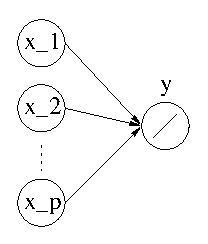
\includegraphics[width=0.45\columnwidth]{figures/linreg.eps}
        \\
        \small
        (a) Linear Regression
    \end{minipage}
    \begin{minipage}{0.48\textwidth}
        \centering
        \psfrag{x_1}[Cc][Cc][1][0]{$x_1$}
        \psfrag{x_2}[Cc][Cc][1][0]{$x_2$}
        \psfrag{x_p}[Cc][Cc][1][0]{$x_p$}
        \psfrag{y}[Cc][Cc][1][0]{$y$}
        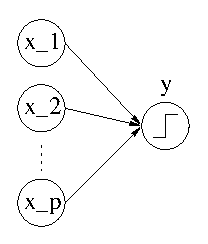
\includegraphics[width=0.45\columnwidth]{figures/perceptron.eps}
        \\
        \small
        (b) Perceptron
    \end{minipage}
    \caption{Illustrations of linear regression and
    perceptron networks. Note that the outputs of these two
    networks use different activation functions.}
    \label{fig:linreg_net}
\end{figure}

We can arrange the input and output units with the described
linear units, as shown in Figure~\ref{fig:linreg_net} (a). With
a proper set of weights, this network then simulates
the unknown function $f$ given an input $x$. 
%Let us denote
%this model as a \textit{simple linear neural network}.

The aim now becomes to find a vector of weights $\vw = [w_1,
\dots, w_p]^\top$ such that the output $u$ of this neural
network estimates the unknown function $f$ as closely as
possible. If we assume Gaussian noise $\epsilon$, this can
be done by minimizing the squared error between the desired
outputs $\left\{ y^{(n)} \right\}$ and the simulated output
$\left\{ u(\vx^{(n)}) \right\}$ with respect to $\vw$:
\begin{align}
    \label{eq:linreg_cost}
    \hat{\vw} = \argmin_{\vw} \sum_{n=1}^N \left( y^{(n)}
    - u\left(\vx^{(n)}\right) \right)^2 + \lambda \Omega
    \left(\vw, D\right),
\end{align}
where $\Omega$ and $\lambda$ are the regularization term and
its strength. Regularization is an oft-used method for
preventing an estimated model from overfitting to training
samples.

If we assume the case of no regularization ($\lambda = 0$),
we can find the analytical solution of $\hat{\vw}$ by a
simple linear least-squares method \citep[see,
e.g.,][]{Golub1996}.  For instance, $\hat{\vw}$ is obtained
by multiplying $\vy = \left[y^{(1)}, y^{(2)}, \dots, y^{(N)}
\right]^\top$ to a pseudo-inverse of $\mX^\top = \left[
\vx^{(1)}, \vx^{(2)}, \dots, \vx^{(N)}\right]^\top$. 

However, when there exists a regularization term, the
problem in Eq.~\eqref{eq:linreg_cost} may not
have an analytical solution depending on the type of the
regularization term. In this case, one must resort to
using an iterative optimization algorithm \citep[see,
e.g.,][]{Fletcher1987}. We iteratively compute updating
directions to update $\vw$ such that eventually $\vw$ will
converge to a solution $\hat{\vw}$ that (locally) minimizes
the cost function.

One exception is the ridge regression which regularizes the
growth of the $L_2$-norm of the weight vector $\vw$ such
that
\begin{align*}
    \Omega(\vw, D) = \sum_{i=1}^p w_i^2.
\end{align*}
In this case, we still have an analytical solution
\begin{align*}
    \hat{\vw} = \left( \mX \mX^\top + \lambda \mI
    \right)^{-1} \mX \vy.
\end{align*}

With other regularization terms, however, it is usual that
there is no analytical solution.  For instance, the
\textit{least absolute shrinkage and selection operator}
(lasso\nomenclature{lasso}{Least absolute shrinkage and selection
operator}) \citep{Tibshirani1994} regularizes the
$L_1$-norm of the weights, and the regularization term 
\begin{align*}
    \Omega(\vw, D) = \sum_{i=1}^p |w_i|.
\end{align*}
does not have an exact analytical solution.

Although we have considered the case of a one-dimensional
output $y$, it is easy to extend this network to predict a
multi-dimensional output. Simply, the network will require
as many output units as the dimensionality of the
output $\vy$. The solution for the weights $\vw$ can be
found in exactly the same way as before by solving the weights
corresponding to each output simultaneously.

This simple linear neural network is highly restrictive in
the
sense that it can only approximate, or simulate, a
\textit{linear} function arbitrary well. When the unknown
function $f$ is not linear, this network will most likely fail
to simulate it.  This is one of the motivations for
considering a deep neural network instead.


\subsection{Perceptron}
\label{sec:perceptron}

The basic idea of the perceptron introduced by
\citet{Rosenblatt1958} is to insert a Heaviside step
function $\phi$ after the summation in a linear unit, where
\begin{align}
    \label{eq:heaviside_func}
    \phi(x) = \left\{ 
    \begin{array}{c c}
        0, &\text{if }x < 0 \\
        1, &\text{otherwise}
    \end{array}
    \right..
\end{align}
The unit $u$ then becomes nonlinear:
\begin{align}
    \label{eq:nonlinear_unit1}
    u(\vx) = \phi\left( 
    \sum_{i=1}^p x_i w_i + b
    \right).
\end{align}
This formula allows us to perform a binary classification,
where each sample is either classified as \textit{negative}
(0) or \textit{positive} (1).
%\footnote{Originally, instead of
%the Heaviside step function, $\phi(x)$ was defined to give
%either $-1$ or $1$.}.
%However, we used $0$ and $1$ for more
%streamlined explanation later.}. 

It is clear from the illustration of a perceptron in
Fig.~\ref{fig:linreg_net} (b) that the perceptron is
identical to the linear regression network except that the
activation function of the output is a nonlinear step
function.
%\citep[see, e.g.,][]{Haykin2009}.

Consider a case where we have again a training set
$D$ of input/output pairs. However, now each output
$y^{(n)}$ is either $0$ or $1$. Furthermore, each $y^{(n)}$
was generated from $\vx^{(n)}$ by an unknown
function $f$, as in Eq.~\eqref{eq:linreg_gen}. As 
before, we want to find a set of weights $\vw$ such that the
perceptron can approximate the unknown function $f$ as
closely as possible.

In this case, this is considered a \textit{classification}
task rather than a \textit{regression} as there is a
finite number of possible values for $y$. The task of the
perceptron is to figure out to which class each sample $\vx$
belongs.

\begin{figure}[t]
    \begin{minipage}{0.48\textwidth}
        \centering
        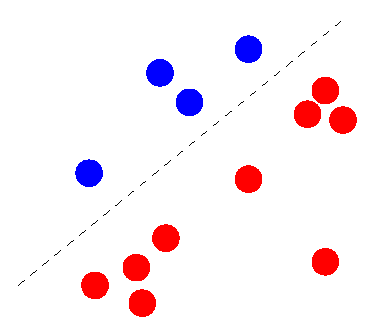
\includegraphics[width=0.75\columnwidth]{figures/linsep.eps}
        \\
        \small
        (a) Linearly separable
    \end{minipage}
    \begin{minipage}{0.48\textwidth}
        \centering
        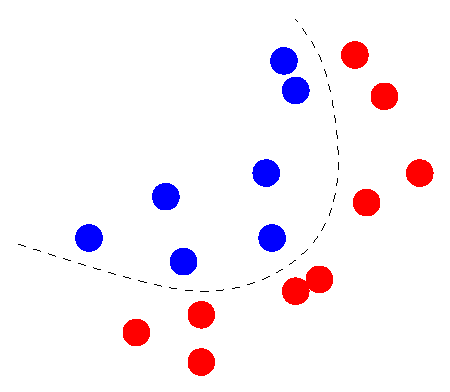
\includegraphics[width=0.75\columnwidth]{figures/nonlinsep.eps}
        \\
        \small
        (b) Nonlinearly separable
    \end{minipage}
    \caption{(a)
    Samples are linearly separable. (b) They are separable,
    but not linearly.}
    \label{fig:linsep}
\end{figure}

A perceptron can perfectly simulate the unknown function
$f$, when the training samples are \textit{linearly}
separable \citep{Minsky1969}.  It means that
there exists a linear hyperplane that separates $\vx^{(n)}$
that belongs to the positive class from those that belong to
the negative class (see Fig.~\ref{fig:linsep}). With a
correct set of weights $\vw^*$, the linear
\textit{separating hyperplane} can be characterized by
\begin{align*}
    \sum_{i=1}^p x_i w_i^* + b^* = 0
\end{align*}

The perceptron learning algorithm was proposed  to estimate
the set of weights
%, assuming $-1$ and $1$ outputs in the
%Heaviside function. 
The algorithm iteratively updates the
weights $\vw$ over $N$ training samples by the following
rule:
\begin{align*}
    \vw \leftarrow \vw + \eta \left[ y^{(n)} -
    u\left(\vx^{(n)}\right)
    \right] \vx^{(n)}.
\end{align*}
This will converge to the correct solution as long as the
given training set is linearly separable.

Note that it is not necessary to use the Heaviside step
function. It is possible to use any other nonlinear
saturating function whose range is limited from above and
below so that it can approximate the Heaviside function.
One such example is a sigmoid function whose range is
$\left[ 0, 1 \right]$:
\begin{align}
    \label{eq:sigmoid}
    \phi(x) = \frac{1}{1 + \exp\left( -x\right)}.
\end{align}
In this case, a given sample $\vx$ is classified positive if
the output is greater than, or equal to, $0.5$, and
otherwise as negative. Another possible choice is a
hyperbolic tangent function whose range is $\left[ -1, 1
\right]$:
\begin{align}
    \label{eq:tanh}
    \phi(x) = \tanh(x).
\end{align}

The set of weights can be estimated in another way by
minimizing the difference between the desired output and the
output of the network, just like in the simple linear neural
network. However, in this case the cross-entropy cost
function \citep[see, e.g.][]{Bishop2006} can be used instead
of the mean squared error:
\begin{align}
    \label{eq:crossentropy_cost}
    \hat{\vw} &= \argmin_{\vw} \sum_{n=1}^N \left(-y^{(n)}
    \log u\left(\vx^{(n)}\right)\right.
    \nonumber\\
    &\phantom{= \argmin_{\vw} \sum_{n=1}^N}\left.-\left(1-y^{(n)}\right)
    \log\left( 1 - 
    u\left(\vx^{(n)}\right)\right)\right) 
    + \lambda \Omega
    \left(\vw, D\right).
\end{align}
Unlike the simple linear neural network, this does not have
an analytical solution, and one needs to use an iterative
optimization algorithm.

As was the case with the simple linear neural network, the
capability of the perceptron is limited. It only works well
when the classes are \textit{linearly} separable \citep[see,
e.g.,][]{Minsky1969}. For instance, a perceptron cannot
learn to compute an exclusive-or
(XOR\nomenclature{XOR}{Exclusive-OR}) function. In this
case, any non-noisy samples from the XOR function are
clearly separable, however, with a nonlinear boundary.

It has been known that a network of perceptrons, having
between the input units and the output unit one or more
layers of nonlinear hidden units that do not correspond to
either inputs or outputs, can solve classification tasks
where classes are not linear separable, such as the XOR
function \citep[see, e.g.,][]{Touretzky1989}. This makes us
consider a \textit{deep} neural network also in the context
of classification.

%In fact, it has been shown that this network, assuming that
%there are enough number of nonlinear, continuous, saturating
%hidden units, requires only a single hidden layer to show a
%universal approximator property \citep{Cybenko1989}. 



\section{Unsupervised Model}
\label{sec:unsupervised_model}

Unlike in supervised learning, we now consider a case where
there is no target value. Hence, the training set $D$ consists of
only input vectors:
\begin{align}
    \label{eq:unsup_train}
D=\left\{ \vx^{(n)} \right\}_{n=1}^N.
\end{align}

Similarly to the supervised case, we may assume that each
$\vx$ in $D$ is a noisy observation of an unknown hidden
variable such that
\begin{align}
    \label{eq:lvm}
    \vx = f(\vh) + \epsilon,
\end{align}
where $\epsilon$ indicates noise. Whereas we aimed
to find the function or mapping $f$ given both input and
output previously in supervised models, our aim here is to
find both the unknown function $f$ and the hidden variables
$\vh \in \RR^q$. This leads to 
\textit{latent variable models} in statistics \citep[see,
e.g.,][]{Murphy2012}.

However, this is not the only way to formulate an
unsupervised model. Another way is to build a model that
learns direct relationships among the input components $x_1,
\dots, x_p$. This does not require any hidden variable, but
still learns an (unknown) structure of the model.


\subsection{Linear Autoencoder and Principal Component Analysis}
\label{sec:linear_autoencoder}

Firstly, we look at the case where hidden variables are
assumed to have generated training samples. In this case, it
is desirable to learn not only an unknown function $f$, but
also another function $g$ which is an inverse function of
$f$. Opposite to $f$, the inverse function $g$ recognizes a
given sample by finding a corresponding state of the hidden
variables\footnote{Note that it is not necessary for $g$ to
be an explicit function. In some models such as sparse
coding in Section~\ref{sec:sparse_coding}, $g$ may be defined
implicitly.}.

Let us start by constructing a neural network with linear
units. There are as many input units as $p$ corresponding to
components of an input vector, denoted by $\vx$, and $q$
linear units that correspond to the hidden variables,
denoted by $\vh$. Additionally, we add another set of $p$
linear units, denoted by $\tilde{\vx}$. We connect directed
edges from $\vx$ to $\vh$ and from $\vh$ to $\tilde{\vx}$.
Each edge $e_{ij}$ which connects the $i$-th input unit
to the $j$-th hidden unit has a corresponding weight
$w_{ij}$. Also, edge $e_{jk}$ which connects the $j$-th
hidden unit to the $k$-th output unit has its weight
$u_{jk}$. See Fig.~\ref{fig:linae} (a) for the illustration.

\begin{figure}[t]
    \begin{minipage}{0.48\textwidth}
        \centering
        \psfrag{x_1}[Cc][Cc][1][0]{$x_1$}
        \psfrag{x_2}[Cc][Cc][1][0]{$x_2$}
        \psfrag{x_p}[Cc][Cc][1][0]{$x_p$}
        \psfrag{y_1}[Cc][Cc][1][0]{$\tilde{x}_1$}
        \psfrag{y_2}[Cc][Cc][1][0]{$\tilde{x}_2$}
        \psfrag{y_p}[Cc][Cc][1][0]{$\tilde{x}_p$}
        \psfrag{h_1}[Cc][Cc][1][0]{$h_1$}
        \psfrag{h_q}[Cc][Cc][1][0]{$h_q$}
        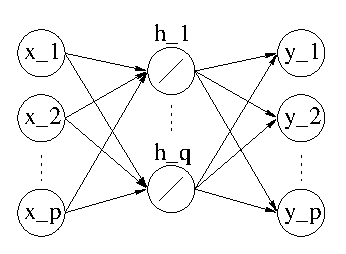
\includegraphics[width=0.75\columnwidth]{figures/linae.eps}
        \\
        \small
        (a) Linear Autoencoder
    \end{minipage}
    \begin{minipage}{0.48\textwidth}
        \centering
        \psfrag{x_1}[Cc][Cc][1][0]{$x_1$}
        \psfrag{x_2}[Cc][Cc][1][0]{$x_2$}
        \psfrag{x_3}[Cc][Cc][1][0]{$x_3$}
        \psfrag{x_p}[Cc][Cc][1][0]{$x_p$}
        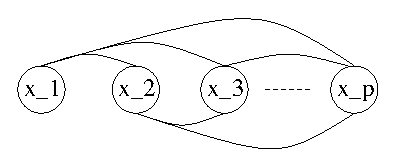
\includegraphics[width=0.8\columnwidth]{figures/hopfield.eps}
        \\
        \small
        (b) Hopfield Network
    \end{minipage}
    \caption{Illustrations of a linear autoencoder and
    Hopfield network. An undirected edge in the Hopfield
    network indicates that signal flows in both ways.}
    \label{fig:linae}
\end{figure}

This model is called a linear autoencoder\footnote{The same
type of neural networks is also called
\textit{autoassociative} neural networks. In this thesis,
however, we use the term \textit{autoencoder} which has
become more widely used recently.}. The encoder of the
autoencoder is
\begin{align}
    \label{eq:linaenc_encoder}
    \vh = f(\vx) = \mW^\top \vx + \vb,
\end{align}
and the decoder is
\begin{align}
    \label{eq:linaenc_decoder}
    \tilde{\vx} = g(\vh) = \mU^\top \vh(\vx) + \vc,
\end{align}
where we uses the matrix-vector notation for simplicity.
$\mW=\left[ w_{ij} \right]_{p \times q}$ are the encoder weights, $\mU =
\left[ u_{jk} \right]_{q \times p}$ the decoder weights, and
$\vb$ and $\vc$ are 
the hidden biases and the visible biases, respectively. It is usual to
call the layer of the hidden units a
\textit{bottleneck}\footnote{Although the term
\textit{bottleneck} implicitly implies that the size of the layer is
smaller than that of either the input or output layers, it
is not necessarily so.}. Note that without loss of
generality we will omit biases whenever it is necessary to
make equations uncluttered.

In this linear autoencoder, the encoder in
Eq.~\eqref{eq:linaenc_encoder} acts as an inverse function
$g$ that recognizes a given sample, whereas the decoder in
Eq.~\eqref{eq:linaenc_decoder} simulates the unknown
function $f$ in Eq.~\eqref{eq:lvm}.

If we tied the weights of the encoder and decoder so that
$\mW=\mU^\top$, we can see the connection between the linear
autoencoder and the principal component analysis (PCA).
Although there are many ways to formulate PCA \citep[see,
e.g.][]{Bishop2006}, one way is to use a minimum-error
formulation\footnote{
Actually the minimum-error formulation minimizes the
mean-squared error $\E\left[ \| \vx - \tilde{\vx} \|_2^2
\right]$ which is in most cases not available for evaluation. The cost
function in Eq.~\eqref{eq:autoencoder_cost} is an
approximation to the mean-squared error using a finite
number of training samples.
}
that minimizes
\begin{align}
    \label{eq:autoencoder_cost}
    J(\TT) =  \frac{1}{2} \sum_{n=1}^N \left\| \vx^{(n)} -
    \tilde{\vx}^{(n)} \right\|_2^2.
\end{align}
The minimum of Eq.~\eqref{eq:autoencoder_cost} is in fact
exactly the solution the linear autoencoder aims to find.  

This connection and equivalence between the linear
autoencoder and the PCA have been noticed and shown by
previous research \citep[see, for
instance,][]{Oja1982,Baldi1989}. However, it should be
reminded that minimizing the cost function in
Eq.~\eqref{eq:autoencoder_cost} by an optimization
algorithm is unlikely to recover the principal components,
but an arbitrary basis of the subspace spanned by the
principal components, unless we explicitly constrain the
weight matrix to be orthogonal.

This linear autoencoder has several restrictions.  The most
obvious one is that it is only able to learn a correct model
when the unknown function $f$ is linear. 
%If $f$ is not a linear function, it is not expected to be
%learned well. 
Secondly, due to its linear nature, it is not possible to
model any hierarchical generative process. Adding more
hidden layers is equivalent to simply multiplying the weight
matrices of additional layers, and this does not help in
any way.

Another restriction is that the number of hidden units $q$
is upper-bounded by the input dimensionality $p$. Although it
is possible to use $q > p$, it will not make any difference,
as it does not make any sense to use more than $p$ principal
components in PCA.  This could be worked around by using
regularization as in, for instance, sparse coding
\citep{Olshausen1996} or independent component analysis
(ICA) with reconstruction cost \citep{Le2011op}. 

As was the case with the supervised models, this encourages
us to investigate more complex, overcomplete models that
have multiple layers of nonlinear hidden units.


\subsection{Hopfield Networks}
\label{sec:hopfield_network}

Now let us consider a neural network consisting of visible
units only, and each visible unit is a \textit{nonlinear},
\textit{deterministic} unit, following
Eq.~\eqref{eq:nonlinear_unit1}, that corresponds to each
component of an input vector $\vx$. We connect each pair of
the units $x_i$ and $x_j$ with an undirected edge $e_{ij}$
that has the weight $w_{ij}$, as in Fig.~\ref{fig:linae} (b).
We add to each unit $x_i$ a bias term $b_i$. Furthermore, let us
define an \textit{energy} of the constructed neural network
as
\begin{align}
    \label{eq:hopfield_energy}
    -E(\vx \mid \TT) = \frac{1}{2} \sum_{i \neq j} w_{ij}
    x_i x_j + \sum_i x_i b_i,
\end{align}
where $\TT = \left( \mW, \vb \right)$.  We call this neural
network a Hopfield network \citep{Hopfield1982}.

The Hopfield network aims to finding a set of weights that
makes the energy of the presented patterns low via the training
set $D=\left\{ \vx^{(1)}, \dots, \vx^{(N)} \right\}$
\citep[see, e.g.,][]{Mackay2002}.
Given a fixed set of weights and an unseen, possibly
corrupted input, the Hopfield network can be used to find a
clean pattern by finding the nearest \textit{mode} in the
energy landscape.

In other words, the weights of the Hopfield network can be
obtained by minimizing the following cost function given a
set $D$ of training samples:
\begin{align}
    \label{eq:hopfield_cost}
    J(\TT) = \sum_{n=1}^N E\left(\left.\vx^{(n)} \right| \TT\right).
\end{align}

The learning rule for each weight $w_{ij}$ can be derived by
taking a partial derivative of the cost function $J$ with
respect to it. The learning rule is 
\begin{align}
    \label{eq:hopfield_grad}
    w_{ij} &\leftarrow w_{ij} - \frac{\eta}{N} \sum_{n=1}^N
    \frac{\partial E\left(\vx^{(n)} \mid \TT
    \right)}{\partial w_{ij}} 
    \nonumber 
    \\ 
    &= w_{ij} +
    \frac{\eta}{N} \sum_{n=1}^N x_i^{(n)} x_j^{(n)} = w_{ij}
    + \eta \left< x_i x_j \right>_\td,
\end{align}
where $\eta$ is a learning rate and $\left< x \right>_P$
refers to the expectation of $x$ over the distribution $P$.
We denote by $\td$ the data distribution from which
samples in the training set $D$ come. Similarly, a
bias $b_i$ can be updated by
\begin{align}
    \label{eq:hopfield_grad_b}
    b_{i} &= b_{i} 
    + \eta \left< x_i \right>_\td.
\end{align}

This learning rule is known as the Hebbian learning rule
\citep{Hebb1949}. This rule states that the weight between
two units, or neurons, increases if they are active
together. After learning, the weight will be strongly
positive, if the activities of the two connected units are
highly correlated. 

With the learned set of weights, we can simulate the network
by updating each unit $x_i$ with
\begin{align}
    \label{eq:hopfield_cond}
    x_i = \phi\left( \sum_{j \neq i} w_{ij} x_j + b_i
    \right),
\end{align}
where $\phi$ is a Heaviside function as in
Eq.~\eqref{eq:nonlinear_unit1}.

It should be noticed that because the energy function in
Eq.~\eqref{eq:hopfield_energy} is not lower bounded and the
gradient in Eq.~\eqref{eq:hopfield_grad} does not depend on
the parameters, we may simply set each weight by
\[
w_{ij} = c \left< x_i x_j \right>_\td,
\]
where $c$ is an arbitrary
%\footnote{
%$c$ may be chosen arbitrarily due to the choice of the
%Heaviside function in Eq.~\eqref{eq:hopfield_cond}.
%}
, positive constant, given a fixed
set of training samples. An arbitrary $c$ is possible, since
the output of \eqref{eq:hopfield_cond} is invariant to the
scaling of the parameters. Hence, the parameters of the
Hopfield network do not require any iterative estimation,
but a single computation.

In summary, the Hopfield network memorizes the training
samples and is able to retrieve them, starting from either a
corrupted input or a random sample. This is one way of
learning an internal structure of a given training set in an
unsupervised manner.

The Hopfield network learns the unknown structure of
training samples. However, it is limited in the sense that
only direct correlations among visible units are modeled. In
other words, the network can only learn second-order
statistics. Furthermore, the use of the Hopfield network is
highly limited by a few fundamental deficiencies including the emergence
of spurious states \citep[for more details,
see][]{Haykin2009}. These encourage us to extend the
model by introducing multiple hidden units as well as
making them stochastic.

\section{Probabilistic Perspectives}
\label{sec:prob_perspective}

All neural network models we have described in this chapter
can be re-interpreted from a probabilistic perspective. This
interpretation helps understanding how neural networks
perform \textit{generative} modeling and \textit{recognize}
patterns in a novel sample.  In this section, we briefly
explain the basic ideas involving probabilistic approaches
to machine learning problems and their relationship to neural
networks.

For more details on probabilistic approaches, we refer
the readers to, for instance, \citep{Murphy2012,Barber2012,Bishop2006}. 

\subsection{Supervised Model}

Let us start by looking at discriminative modeling from
the probabilistic perspective. Again, we assume that a set
$D$ of $N$ input/output pairs, as in
Eq.~\eqref{eq:set_disc}, is given. The same model in
Eq.~\eqref{eq:linreg_gen} is used to describe how the set
$D$ was generated. In this case, we can directly plug in a
probabilistic interpretation.

Let each component $x_i$ of $\vx$ be a random variable, but
for now fixed to a given value. Also, we assume that the
observation of $y$ is corrupted by additive noise
$\epsilon$ which is another random variable.
%$\epsilon$ is another random variable. 
Then, the aim of
discriminative modeling in a probabilistic approach is to
estimate or approximate the conditional distribution of
yet another random variable $y$ given the input $\vx$ and
the noise $\epsilon$ parameterized\footnote{It is
possible to use non-parametric approaches, such as Gaussian
Process (GP\nomenclature{GP}{Gaussian Process}) \citep[see, e.g.,][]{Rasmussen2006}, which do
not have in principle any explicit parameter. However, we may safely
use the parameters $\TT$ by including the hyper-parameters
of, for instance, kernel functions and potentially even
(some of) the training samples.} by $\TT$, that is, ${p(y \mid \vx,
\TT)}$.

With the estimated parameters $\tilde{\TT}$, the prediction
of the output $\hat{y}$ given a new sample $\vx$ can be
computed from the conditional distribution $p(y \mid
\vx, \tilde{\TT})$. It is typical to use the mean of the
distribution as a prediction and its variance as a
confidence.

\subsubsection{Linear Regression}

A probabilistic model equivalent to the previously described
linear regression network can be easily built by assuming
that the noise
$\epsilon$ follows a Gaussian distribution with zero mean
and its variance is fixed to $s^2$. Then, the conditional
distribution of $y$ given a fixed input $\vx$ becomes
\begin{align*}
    p(y \mid \vx, s^2) = \NN \left( y \left| \sum_{i=1}^p
    x_i w_i + b, s^2\right.\right),
\end{align*}
where $\NN \left( y \left| m, s^2\right.\right)$ is a
probability density of the scalar variable $y$ following a Gaussian distribution
with the mean $m$ and variance $s^2$. A linear relationship
between the input and output variables has been assumed in
computing the mean of the distribution.

The parameters $w_i$ and $b$ can be found by maximizing
the log-likelihood function
\begin{align}
    \label{eq:linreg_ll}
    \LL(\vw, b) = -\sum_{n=1}^N \frac{\left( y^{(n)} -
    \sum_{i=1}^p x_i^{(n)} w_i - b \right)^2}{2 s^2} +
    \text{C},
\end{align}
where the constant $\text{C}$ does not depend on any parameter.
This way of estimating $\hat{w}_i$ and $\hat{b}$ to
maximize $\LL$ is called maximum-likelihood estimation
(MLE).

If we assume a fixed constant $s^2$, maximizing $\LL$ is
equivalent to minimizing
\begin{align*}
    \sum_{n=1}^N \left( y^{(n)} -
    u(\vx^{(n)})\right)^2
\end{align*}
using the definition of the output of a linear unit $u(\vx)$
from Eq.~\eqref{eq:linear_unit}. This is identical to the
cost function of the linear regression network given in
Eq.~\eqref{eq:linreg_cost} without a regularization term. 

A regularization term can be inserted by considering the
parameters as random variables. When each weight parameter
$w_i$ is given a prior distribution, the log-posterior
distribution $\log p(\vw \mid \vx, y)$ of the weights can be
written, using Bayes' rule\footnote{Bayes' rule states
that
\begin{align}
    \label{eq:bayes_rule}
    p(X \mid Y) = \frac{p(Y \mid X) p(X)}{p(Y)},
\end{align}
where both $X$ and $Y$ are random variables. One
interpretation of this rule is that the posterior
probability of $X$ given $Y$ is proportional to the product
of the likelihood (or conditional probability) of $Y$ given
$X$ and the prior probability of $X$. Hence, if both the
conditional and prior distributions are specified, the
posterior probability can be evaluated as their product, up
to the normalization constant or evidence $p(Y)$.}, as
\begin{align*}
    \log p(\vw \mid \vx, y) = \log p(y \mid \vx, \vw) + \log
    p(\vw) + \text{const.},
\end{align*}
where the constant term does not depend on the weights. If,
for instance, the prior distribution of each weight $w_i$ is
a zero-mean Gaussian distribution with its variance fixed to
$\tfrac{1}{2\lambda}$, the log-posterior distribution given
a training set $D$ becomes
\begin{align*}
    \log p\left(\vw \left| \left\{ (\vx^{(n)}, y^{(n)})
    \right\}_{n=1}^N \right. \right) = \LL(\vw, b) - \lambda
    \sum_{i=1}^p w_i^2.
\end{align*}
Maximizing this posterior is equivalent to ridge regression
\citep{Hoerl1970}. When the log-posterior is maximized
instead of the log-likelihood, we call it a
maximum-a-posteriori estimation
(MAP\nomenclature{MAP}{Maximum-a-posteriori estimation}), or
in some cases, penalized maximum-likelihood estimation
(PMLE).


\subsubsection{Logistic Regression: Perceptron}
\label{sec:log_reg}

As was the case in our discussion on perceptrons in
Section~\ref{sec:perceptron}, we consider a binary
classification task. 

Instead of Eq.~\eqref{eq:linreg_gen} where it was assumed
that the output $y$ was generated from an input $\vx$
through an unknown function $f$, we can think of a
probabilistic model where the sample $\vx$ was generated
according to the conditional distribution given its
label\footnote{ A \textit{label} of a sample tells to which
\textit{class} the sample belongs. Often these
two terms are interchangeable.
}
$y$, where $y$ was chosen according to the prior
distribution.  In this case, we assume that we know the
forms of the conditional and prior distributions \textit{a
priori}. See Fig.~\ref{fig:naive_bayes} (a) for the
illustration of this model, which is often referred to as the
naive Bayes model \citep[see, e.g.,][]{Bishop2006}.

%The model in Fig.~\ref{fig:naive_bayes} (a) is called the
%naive Bayes model. In the naive Bayes model it is explicitly
%assumed that the input components are mutually independent
%when the corresponding label $y$ is observed \citep[see,
%e.g.,][]{Bishop2006}.

\begin{figure}[t]
    \begin{minipage}{0.48\textwidth}
        \centering
        \psfrag{x_1}[Cc][Cc][1][0]{$x_1$}
        \psfrag{x_2}[Cc][Cc][1][0]{$x_2$}
        \psfrag{x_p}[Cc][Cc][1][0]{$x_p$}
        \psfrag{y}[Cc][Cc][1][0]{$y$}
        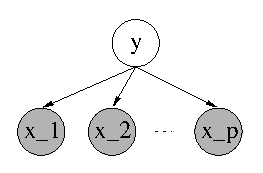
\includegraphics[width=0.65\columnwidth]{figures/naiveb.eps}
    \end{minipage}
    \begin{minipage}{0.48\textwidth}
        \centering
        \psfrag{x_n}[Bc][Bc][1][0]{$\vx^{(n)}$}
        \psfrag{h_n}[Cc][Cc][1][0]{$\vh^{(n)}$}
        \psfrag{s}[Cc][Cc][1][0]{$\sigma^2$}
        \psfrag{N}[Cc][Cc][1][0]{$N$}
        \psfrag{W}[Cc][Cc][1][0]{$\mW$}
        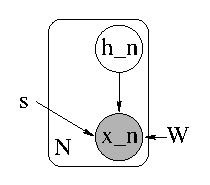
\includegraphics[width=0.65\columnwidth]{figures/ppca.eps}
    \end{minipage}

    \vspace{2mm}
    \begin{minipage}{0.48\textwidth}
        \centering
        \small
        (a) Naive Bayes
    \end{minipage}
    \begin{minipage}{0.48\textwidth}
        \centering
        \small
        (b) Probabilistic PCA
    \end{minipage}
    \caption{Illustrations of the naive Bayes classifier and
    probabilistic principal component analysis. The naive Bayes
    classifier in (a) describes the conditional independence
    of each component of input given its label. In both
    figures, the random variables are denoted with circles
    (a gray circle indicates an \textit{observed}
    variables), and other parameters are without surrounding
    circles. The plate indicates that there are $N$ copies
    of a pair of $\vx^{(n)}$ and $\vh^{(n)}$. For details on
    probabilistic graphical models, see, for instance,
    \citep{Bishop2006}.}
    \label{fig:naive_bayes}
\end{figure}

Based on this model, the aim is to find a class, or a label,
that has the highest posterior probability given a sample.
In other words, a given sample belongs to a class 1, if
\begin{align*}
    p(y = 1 \mid \vx) \geq \frac{1}{2},
\end{align*}
since
\begin{align*}
    p(y = 1 \mid \vx) + p(y = 0 \mid \vx) = 1
\end{align*}
in the case of a binary classification.

Using the Bayes' rule in Eq.~\eqref{eq:bayes_rule}, we may
write the posterior probability as
\begin{align*}
    p(y = 1 \mid \vx) &= \frac{p(\vx \mid y = 1) p(y = 1)}{
    p(\vx \mid y = 1)p(y = 1) + p(\vx \mid y = 0) p(y = 0)}
    \\
    &= \frac{1}{1 + \frac{p(\vx \mid y = 0) p(y = 0)}{p(\vx
    \mid y = 1) p(y = 1)}} \\
    &= \frac{1}{1 + \exp\left(-\log \frac{p(\vx \mid y = 1) p(y = 1)}{p(\vx
    \mid y = 0) p(y = 0)}\right)}.
\end{align*}
It is easy to see that the posterior probability takes the
form of a sigmoid function with an input 
\[
a = \log \frac{p(\vx \mid y = 1) p(y = 1)}{p(\vx
    \mid y = 0) p(y = 0)}.
\]

A logistic regression approximates this input $a$ with a
weighted linear sum of the components of an input. The
posterior probability of $y=1$ is then
\begin{align*}
    u(\vx)  = p(y = 1 \mid \vx, \TT) = \phi\left( \mW^\top \vx + b
    \right),
\end{align*}
where $\TT = (\mW, b)$ is a set of parameters. We put
$u(\vx)$ to show the equivalence of the posterior
probability to the nonlinear output unit used in the
perceptron (see Eq.~\eqref{eq:nonlinear_unit1}). Since the
posterior distribution of $y$ is simply a Bernoulli random
variable, we may write the log-likelihood of the
parameters $\TT$ as
\begin{align}
    \label{eq:logreg_ll}
    \LL(\TT) = \sum_{n=1}^N y^{(n)} \log u(\vx^{(n)}) + (1 -
    y^{(n)})\log (1 - u(\vx^{(n)})).
\end{align}

This is identical to the cross-entropy cost function
in Eq.~\eqref{eq:crossentropy_cost} that was used
to train a perceptron, except for the regularization term.
The regularization term can be, again, incorporated by
introducing a prior distribution to the parameters, as was
done with the probabilistic linear regression in the
previous section.


\subsection{Unsupervised Model}

The aim of unsupervised learning in a probabilistic
framework is to let the model approximate a distribution
$p(\vx \mid \TT)$ of a given set of training samples,
parameterized by $\TT$. As was the case without any
probabilistic interpretation, two approaches are often used.
The first approach utilizes a set of hidden variables to
describe the relationships among visible variables. On the
other hand, the other approach does not require
introducing hidden variables.

\subsubsection{Principal Component Analysis and
Expectation-Maximization}
\label{sec:ppca}

PCA can be viewed in a probabilistic perspective
\citep[see, e.g.,][]{Tipping1999,Roweis1998} by considering
both $\vx$ and $\vh$ in Eq.~\eqref{eq:lvm} as random
variables and assuming that $f$ is a linear function
parameterized by the projection matrix $\mW$. The noise term
$\epsilon$ follows a zero-mean Gaussian distribution with
its variance $\sigma^2$. Furthermore, we may assume that the
training samples $\vx^{(n)}$ are centered so that their
mean is zero\footnote{This is not necessary, but for
simplicity, it is assumed here.}.

The hidden variables $\vh$ follow a zero-mean
unit-covariance multivariate Gaussian distribution such that
\begin{align*}
    \vh \sim \NN(\vzero, \mI),
\end{align*}
and the conditional distribution over $\vx$ given $\vh$ is
also a multivariate Gaussian with a diagonal covariance:
\begin{align*}
    \vx \mid \vh \sim \NN(\mW \vh, \sigma^2 \mI).
\end{align*}
This is illustrated in Fig.~\ref{fig:naive_bayes} (b).

The aim is to estimate $\mW$ and $\sigma^2$ by maximizing
the marginal log-likelihood, given by
\begin{align}
    \label{eq:ppca_mll}
    \LL(\TT) = \sum_{n=1}^N \log \int_{\vh} p(\vx^{(n)} \mid \vh)
    p(\vh) \dd{\vh},
\end{align}
where $\TT=\left( \mW, \sigma^2 \right)$. Because both the prior
distribution of $\vh$ and the conditional distribution of
$\vx \mid \vh$ are Gaussian distributions, 
the marginal distribution of $\vx$ is also a Gaussian
distribution with the following sufficient statistics:
\begin{align*}
    \E\left[ \vx \right] &= 0,\\
    \cov\left[ \vx \right] &= \mC = \mW \mW^\top + \sigma^2 \mI.
\end{align*}

In this case, \citet{Tipping1999} showed that all the 
stationary points of the marginal log-likelihood function
$\LL$ are given by
\[
\hat{\mW} = \mU_q \left( \mL_q - \sigma^2 \mI \right)^{1/2}
\mR
\]
and
\[
\hat{\sigma}^2 = \frac{1}{p - q} \sum_{i=q+1}^p \lambda_i,
\]
where $\mU_q$, $\mL_q$ and $\lambda_i$ are any subset of
$q$ eigenvectors of the data covariance, the diagonal matrix
of corresponding eigenvalues, and the $i$-th eigenvalue,
respectively. $\mR$ is an arbitrary orthogonal
matrix\footnote{
Any orthogonal matrix can be used as $\mR$, since it does
not change the sufficient statistics, specifically the
covariance of the observation, as $\mW\mR\left( \mW\mR\right)^\top
= \mW\mR \mR^\top \mW^\top = \mW\mW^\top$.
}.
Furthermore, in \citep{Tipping1999}, it was shown that $\LL$
is maximal when the $q$ \textit{largest} eigenvectors and
eigenvalues of the data covariance were used.

However, we are more interested in solving PCA using
the expectation-maximization
(EM\nomenclature{EM}{Expectation-Maximization}) algorithm
\citep{Dempster1977}, which was proposed by
\citet{Roweis1998}.  It will make the connection to the
linear autoencoder introduced in
Section~\ref{sec:linear_autoencoder} more clear.

The EM algorithm is an iterative algorithm used to find a
maximum-likelihood estimate when the probabilistic model
has a set of unobserved, hidden variables. Let us state the
algorithm based on \citep{Neal1999,Bishop2006}.

We first note that the marginal log-likelihood in
Eq.~\eqref{eq:ppca_mll} can be decomposed by
\begin{align}
    \label{eq:mll_decom}
    \LL(\TT) = \sum_{n=1}^N \LL^{(n)}(\TT) = \sum_{n=1}^N
    \LL_{Q^{(n)}}(\TT) + \KL(Q^{(n)} \| P^{(n)}),
\end{align}
where
\begin{align}
    \label{eq:mll_post}
    \LL_{Q^{(n)}}(\TT) = \E_{Q^{(n)}} \left[ \log
    p(\vx^{(n)}, \vh \mid
    \TT)\right] + \HH(Q^{(n)})
\end{align}
and
\begin{align}
    \label{eq:kldiv}
    \KL(Q^{(n)} \| P^{(n)}) = -\E_{Q^{(n)}} \left[ \log
    \frac{p(\vh \mid \vx^{(n)},
    \TT)}{Q^{(n)}(\vh)} \right],
\end{align}
and $P^{(n)}$ and $Q^{(n)}$ denote the true posterior distribution
$p(\vh \mid \vx^{(n)}, \TT)$ and any arbitrary distribution,
respectively. $\KL(Q \| P)$ is a Kullback-Leibler
(KL\nomenclature{KL}{Kullback-Leibler divergence})
divergence that measures the difference between two
distributions $Q$ and $P$ \citep{Kullback1951}.

The first term is a complete-data log-likelihood over the
posterior distribution of $\vh$ given $\vx^{(n)}$, and the
second term is a KL divergence between a distribution
$Q^{(n)}$ and the posterior distribution over $\vh$.
$\HH(Q)$ is an entropy functional of the distribution $Q$.
%which is independent from
%$\TT$ so that we can ignore the term.

It is easy to see that $\LL_{Q^{(n)}}(\TT)$ is a lower bound
of $\LL^{(n)}(\TT)$ for all $n$ in Eq.~\eqref{eq:mll_decom},
since the KL-divergence $\KL(Q^{(n)}\| P^{(n)})$ is always
non-negative. From this clearly $\sum_{n=1}^N
\LL_{Q^{(n)}}(\TT)$ is a lower bound of the marginal
log-likelihood $\LL(\TT)$. The lower bound is
equal to the marginal log-likelihood when an arbitrary
distribution $Q^{(n)}$ is equivalent to the posterior distribution
($\KL(Q^{(n)} \| P^{(n)}) = 0$) for all the training
samples.

From this decomposition, we now state the EM algorithm
consisting of two steps; expectation (E) and maximization
(M) steps:
\begin{enumerate}
    \itemsep 0em
    \item[(E)] Maximize $\LL_Q(\TT)$ with respect to $Q(\vh)$
        while $\TT$ is fixed.
    \item[(M)] Maximize $\LL_Q(\TT)$ with respect to $\TT$
        while $Q(\vh)$ is fixed.
\end{enumerate}
In other words, we repeatedly update the approximate
posterior distribution $Q$ and the set of parameters $\TT$
sequentially. 

Since the original $\LL(\TT)$ is not dependent on the choice
of $Q$, the E-step effectively minimizes the KL-divergence
between $Q$ and the true posterior distribution. This is
equivalent to saying that $Q(\vh)$ becomes a better
approximate of the true posterior distribution
$p(\vh\mid\vx,\TT)$.

In probabilistic PCA, the E-step simply estimates the
sufficient statistics of the posterior distribution $p(\vh
\mid \vx, \tilde{\TT})$ with the fixed set of parameters
$\tilde{\TT}$.
The posterior distribution follows in this case again a
Gaussian distribution, and the sufficient statistics are
\begin{align*}
    \E \left[ \vh^{(n)} \right] &= (\tilde{\mW}^\top
    \tilde{\mW} + \tilde{\sigma}^2
    \mI)^{-1} \tilde{\mW}^\top \vx^{(n)} \\
    \E \left[ \vh^{(n)} {\vh^{(n)}}^\top \right] &=
    \tilde{\sigma}^2 (\tilde{\mW}^\top \tilde{\mW} +
    \tilde{\sigma}^2
    \mI)^{-1} + \E\left[\vh^{(n)}\right] \E\left[ \vh^{(n)}
    \right]^\top.
\end{align*}
These are simplified in the limiting case of $\sigma^2 \to
0$ as
\begin{align}
    \label{eq:ppca_post_ss_mean}
    \E \left[ \vh^{(n)} \right] &= \tilde{\mW}^\top \vx^{(n)} \\
    \label{eq:ppca_post_ss_cov}
    \E \left[ \vh^{(n)} {\vh^{(n)}}^\top \right] &=
    \E\left[\vh^{(n)}\right] \E\left[ \vh^{(n)}
    \right]^\top.
\end{align}
The mean of each hidden unit in
Eq.~\eqref{eq:ppca_post_ss_mean} clearly corresponds to the
encoder of a linear autoencoder in
Eq.~\eqref{eq:linaenc_encoder}.

Again, in the limit of $\sigma^2 \to 0$, at the M-step, the
weights $\mW$ that maximize $\LL_{\tilde{Q}}(\TT)$ with the fixed
$\tilde{Q}$ from the E-step, are obtained by
\begin{align}
    \label{eq:ppca_m_weights}
    \mW = \left[ \sum_{n=1}^N \vx^{(n)} \E\left[ \vh^{(n)}
    \right]^\top \right]\left[ \sum_{n=1}^N \E\left[
    \vh^{(n)} \right] \E\left[ \vh^{(n)} \right]^\top
    \right]^{-1}.
\end{align}
We ignore $\sigma^2$ as we consider the case of $\sigma^2 \to
0$.  This update corresponds to minimizing the squared
reconstruction error between $\vx^{(n)}$ and $\mW
\E\left[\vh^{(n)}\right]$.

%This EM iteration is equivalent to the fixed-point iteration
%of the weights matrix $\mW$ that minimizes the following
%cost function 
%\[
%\sum_{n=1}^N \left( \vx^{(n)} - \mW \left(\mW^\top
%\vx^{(n)}\right)\right)^2,
%\]
%which is identical to the cost function of the linear
%autoencoder in Eq.~\eqref{eq:autoencoder_cost}. We omitted
%biases without loss of generality.

This gives us another possible interpretation of the
components of an autoencoder, in general. The encoder
\textit{infers} the state of the hidden variables given an
input, and the decoder \textit{generates} a visible sample
given a state of the hidden variables.

\subsubsection{Fully-Visible Boltzmann Machines}
\label{sec:fvbm}

The Hopfield network described in
Section~\ref{sec:hopfield_network} becomes
\textit{stochastic} if each unit is stochastic.
By a \textit{stochastic} unit, we mean that the activity of
the unit is not deterministically decided based on the
output of each unit but is randomly sampled from its
distribution.  A resulting stochastic version of the Hopfield
network is called a Boltzmann machine\footnote{ An
equivalent model of the fully-visible Boltzmann machine,
called an Ising model, is used in physics to investigate a
phase transition of a large system consisting of small,
locally interacting particles. We refer any interested
reader to \citep[][and references therein]{Cipra1987}.},
proposed by \citet{Ackley1985}. 

Instead of the energy of the Hopfield network, the Boltzmann
machine is defined by a probability distribution. The
probability of a state $\vx$ follows a \textit{Boltzmann
distribution}\footnote{The Boltzmann distribution is often
referred to as a \textit{Gibbs distribution} as well. This
distribution was discovered for describing the statistical
distribution of any macroscopic (small) part of a large
closed system in statistical physics \citep[see,
e.g.,][]{Landau1980}. Under this distribution, the
probability of a state $\vx$ is
\begin{align*}
    p(\vx) = \frac{1}{Z} \exp\left\{ -\frac{E(\vx)}{T}
    \right\},
\end{align*}
where $T$ is the temperature of the system and $Z$ is a
normalization constant which does not depend on $E(\vx)$.
}
(with the temperature $T$ fixed to $1$) which is
defined by
\begin{align}
    \label{eq:bm}
    p(\vx \mid \TT) = \frac{1}{Z(\TT)} \exp \left\{
    -E\left(\vx \mid \TT \right)\right\},
\end{align}
where $Z(\TT)=\sum_{\vx} \exp\left\{ -E(\vx \mid \TT)
\right\}$ is a normalization constant that ensures the
probabilities sum up to one. Although it is possible to have
hidden units that do not correspond to any component in the
input of a Boltzmann machine, we do not consider them in this
section.

The conditional probability of a unit $x_i$ given the state
of all other units $\vx_{-i}$ is
\begin{align}
    \label{eq:bm_cond}
    p(x_i = 1 \mid x_1, \cdots, x_{i-1}, x_{i+1}, \dots ,x_N,
    \TT) = \phi\left( \sum_{j \neq i} w_{ij} x_j + b_i
    \right),
\end{align}
where $\phi$ is a sigmoid function. It is easy to see the
equivalence of this equation and
Eq.~\eqref{eq:hopfield_cond} after substituting the
Heaviside function with the sigmoid function. 

Since it is possible to define a proper distribution,
learning the weights is done by maximizing the
log-likelihood. The log-likelihood function is defined to be
\begin{align}
    \label{eq:fvbm_ll}
    \LL(\TT) &= \sum_{n=1}^N \log p(\vx^{(n)} \mid \TT) 
    \nonumber
    \\
    &= \sum_{n=1}^N -E\left( \vx^{(n)} \mid \TT \right) -
    \log Z(\TT).
\end{align}

The learning rule of the Boltzmann machine is quite similar
to that of the Hopfield network. However, due to the
existence of the normalization constant $Z(\TT)$, an
additional term appears. The learning rule for the weight
$w_{ij}$ of the Boltzmann machine is
\begin{align}
    \label{eq:fvbm_update}
    w_{ij} \leftarrow w_{ij} + \eta \left( \left< x_i
    x_j\right>_\td - \left< x_i x_j \right>_\tf \right),
\end{align}
where $\td$ and $\tf$ refer to the data distribution defined
by the training set $D$ and the model distribution defined
by the Boltzmann machine (see Eq.~\eqref{eq:bm}),
respectively\footnote{
For the derivations of the conditional distribution in
Eq.~\eqref{eq:bm_cond} and the gradient in
Eq.~\eqref{eq:fvbm_update}, see, for instance,
\citep{Cho2011t}.
}.

Although computing the statistics of the distribution
learned by the Boltzmann machine, called the model distribution,
is computationally intractable, one can approximate it with
Markov Chain Monte Carlo (MCMC\nomenclature{MCMC}{Markov Chain
Monte Carlo}) sampling \citep[see,
e.g.,][]{Neal1993}.
As the conditional distribution of each unit can be exactly
and efficiently computed by Eq.~\eqref{eq:bm_cond}, it is
possible to gather unbiased samples from the model
distribution by Gibbs sampling introduced by
\citet{Geman1984}. More on how to compute the statistics of
the model distribution will be discussed later in
Section~\ref{sec:mcmc}.

Even though each unit is now stochastic and a
valid probability distribution of input samples can be
learned, the same limitation of the Hopfield network
persists in the fully-visible Boltzmann machine. It also can
only model the second-order statistics of the training
samples. Hence, this again encourages us to consider
introducing hidden units.

\section{What Makes Neural Networks Deep?}
\label{sec:deep_conditions}

The neural networks discussed in this chapter are
\textit{shallow} in the sense that the number of layers of
units, regardless of their types, is usually at most two.
Logistic regression, for instance, consists of two layers
corresponding to input and output layers. A linear
autoencoder or PCA consists of an input layer and a single
hidden layer, considering that the input and the output
layers of the linear autoencoder represent the same
variable. Then we must ask ourselves: \textit{what must a
neural network satisfy in order to be called a \textbf{deep
neural network}?}

A straightforward requirement of a deep neural network
follows from its name. A deep neural network is
\textit{deep}. That is, it has
multiple, usually more than three, layers of units.
However, this does not fully characterize the deep neural
networks we are interested in.

In essence, we say that a neural network is deep 
when the following two conditions are met \citep[see, e.g.,][]{Bengio2007a}:
\begin{enumerate}
    \itemsep 0em
    \item The network can be extended by adding layers consisting of multiple units.
    \item The parameters of each and every layer are trainable.
    %\item The performance of the network on a target task benefits from unsupervised modeling of input data.
\end{enumerate}

From these conditions, it should be understood that there is
no absolute number of layers that distinguishes deep neural
networks from shallow ones. Rather, the depth of a deep
neural network grows by a generic procedure of adding and
training one
or more layers, until it can properly perform a
target task with a given dataset. In other words,
\textit{the data decide how many layers a deep neural network
needs}\footnote{Yoshua Bengio, personal communication}. 

One important consequence of the first condition is that
since the units in an added layer use the activations of the
units in the existing lower layers to compute their own
activations, the activations of the units in the lower
layers are \textit{shared}.  In other words, there exist
more than one computational path from the input layer to a
unit in the added, upper layers.

%An additional 


%The last condition may only be satisfied when the target
%task of a deep neural network is \textit{not} generative
%modeling of a training set. For instance, a deep neural
%network can benefit from generative modeling when, in fact,
%the network will be used for classification.

In the following chapters of this thesis, we will look at
deep neural networks that have become widely used recently,
and discuss how they satisfy these conditions given above.
For each of those networks, the structure as well as
learning algorithms to estimate its parameters will be
presented and explained.

\section{Learning Parameters: Stochastic Gradient Method}
\label{sec:stochastic_grad}

Before ending this chapter and moving on to discuss deep
neural networks, we briefly look at one of the most widely
used techniques for learning parameters of a neural network,
or any parameterized machine learning model.  This can be
applied not only to the simple models introduced
earlier in this chapter, but also to the deep neural networks
that will be discussed later.

The cost functions, or \textit{negative} log-likelihood
functions, we discussed in this chapter so far (See
Eqs.~\eqref{eq:linreg_cost}, \eqref{eq:crossentropy_cost},
\eqref{eq:autoencoder_cost}, \eqref{eq:hopfield_cost},
\eqref{eq:linreg_ll}, \eqref{eq:logreg_ll},
\eqref{eq:ppca_mll} and \eqref{eq:fvbm_ll}), can be
generalized as the average of losses over training samples such
that
\begin{align}
    \label{eq:slt_emp_cost}
    R_e(\TT) = \frac{1}{N} \sum_{n=1}^N L(\vx^{(n)}, \TT),
\end{align}
where $\vx^{(n)}$ can be either a sample-label pair
(supervised models) or just a sample (unsupervised models).
$L(\vx, \TT)$ is a non-negative loss function.

If we follow the approach of the statistical learning theory
\citep[see, e.g.][]{Vapnik1995}, the empirical cost function
$R_e$ approximates the expected cost function 
\begin{align}
    \label{eq:slt_exp_cost}
    R(\TT) = \E_{\vx} \left[ L(\vx, \TT) \right] = \int
    p(\vx) L(\vx, \TT) d\vx,
\end{align}
where $p(\vx)$ is the probability of $\vx$ or the data
distribution. Clearly, $R(\TT)$ cannot be evaluated directly
as the distribution from which the training samples $\left\{
\vx^{(1)}, \dots, \vx^{(N)} \right\}$ were sampled is
\textit{unknown}, while the empirical cost $R_e(\TT)$
can be in many cases exactly computed.

However, there is another way to look at the empirical cost
function. Instead of considering a set of training samples
as an initially \textit{given} fixed set, we may consider
them as a sequence of sampled points from an unknown
data distribution $D(\vx)$. For instance, at time $t$ we
approximate the expected cost function $R(\TT)$ by
\begin{align*}
    R(\TT) \approx R_e^{\qexp{t}}(\TT) = \frac{1}{t}
    \sum_{i=1}^t L(\vx^{\qexp{i}}, \TT),
\end{align*}
where $\vx^{\qexp{i}}$ is the sample collected from $D$ at time
$i$, and we denote the empirical cost at time $t$ by
$R_e^{\qexp{t}}$. As $t\to\infty$, the empirical cost will
converge to $R(\TT)$, assuming that the samples are unbiased.

Under this perspective, we may justify using the stochastic
approximation method initially proposed by
\citet{Robbins1951}.  According to this method, the set of
parameters $\TT$ that minimizes the expected loss can be
found by updating them iteratively by
\begin{align}
    \label{eq:sgd_grad}
    \TT^{\qexp{t+1}} = \TT^{\qexp{t}} - \eta_{\qexp{t}}
    \nabla_{\TT} L(\vx^{\qexp{t}},
    \TT^{\qexp{t}}),
\end{align}
where the superscript $\qexp{t}$ indicates the value of the
variable at time $t$. \citet{Bottou1998} provides a proof of
almost sure convergence of this procedure to the true
solution with a \textit{convex} $R(\TT)$, with the following
constraints on the learning rate
\begin{align}
    \label{eq:sgd_lr_cond1}
    \sum_{t=1}^\infty \eta_{\qexp{t}}^2 < \infty, \\
    \label{eq:sgd_lr_cond2}
    \sum_{t=1}^\infty \eta_{\qexp{t}} = \infty,
\end{align}
assuming that $\E_\vx \left[ \nabla_{\TT} L(\vx, \TT) \right] =
\nabla_\TT R(\TT)$. We call $\nabla_{\TT} L(\vx^{\qexp{t}},
\TT^{\qexp{t}})$ a \textit{sample gradient} at time $t$.

Furthermore, \citet{Bottou1998} also proves a more general
case where the convexity of $R(\TT)$ is \textit{not}
assumed. With some more assumptions, he was able to show
that the iterations in Eq.~\eqref{eq:sgd_grad} converge to
one of the extremal points of $R(\TT)$ that include
global/local minima and saddle points.

All these proofs, however, essentially require that the
number of training samples approaches infinity, assuming
that $\vx$ is continuous. In most of machine learning tasks,
this assumption does not hold. However, it is possible to
use this approach by choosing a single sample, or a (mini-)batch of
a fixed-number of samples, at each iteration from the whole
training set uniform-randomly to compute the sample
gradient. It is also a usual practice to simply cycle
through all (randomly shuffled) training samples several
times.

This method of iteratively updating parameters using the
stochastic iterate in Eq.~\eqref{eq:sgd_grad} is often
referred to as a \textit{stochastic gradient method}. As one
may easily guess from its name, its deterministic
counterpart is a simple, \textit{batch} gradient method.

The most important advantage of using this method is that
the computational resource required at each iteration can be
bounded by a constant with respect to the number of training
samples. A batch steepest gradient method requires time
linearly proportional to the number of all training samples.
On the other hand, it takes constant time to compute a stochastic
gradient with respect to the
number of training samples. Furthermore, since only few samples are used for
computing a stochastic gradient, the memory requirement is
also much smaller than in the batch method.

Many studies \citep[see, e.g.,][]{Bottou2008,Bottou2004}
have shown that the stochastic gradient method converges to
at least a general area in the parameter space with a
relatively low cost function very rapidly. Furthermore, some
even argued that it is easier to achieve a better solution
in terms of the expected cost rather than the empirical cost
with the stochastic gradient method compared to the batch
gradient method in the case of neural networks
\citep{Lecun1998a}.

Hence, when we talk about estimating
parameters in this thesis, it is implicitly assumed that the stochastic
gradient method is used together with a cost, or objective
function of each model. Most arguments on the advantages and
disadvantages of learning algorithms specific to different
neural networks presented later will also assume that the
stochastic gradient method is used.

Recently there have been many approaches that try to
overcome the weaknesses of the naive stochastic gradient
method, such as the slow convergence rate and inability to
easily escape from a plateau or a saddle point.  Tonga,
proposed by \citet{Roux2008a}, speeds up the convergence of
the stochastic gradient method by utilizing an online
approximation to the natural gradient.
\citet{Schraudolph2007} proposed an online variant of the
popular Quasi-Newton method.
Also, \citet{Le2011} compared the performances of various
second-order optimization methods in training deep neural
networks against the stochastic gradient descent.

However, we will not further discuss on the stochastic
gradient method and its extensions, as they are out of the
scope of this thesis.




\chapter{Feedforward Neural Networks: \\{\small Multi-layer
Perceptron and Deep Autoencoder}}
\label{chap:ffnn}

In this chapter, we describe deep feedforward neural
networks. A feedforward neural network consists of units
that are connected to each other with directed edges, where
each edge propagates the activation of one unit to another.
The network is \textit{feedforward} in the sense that there
are no feedback connections in the network, which makes it
efficient to evaluate the activations of all units in the
network with a single sweep from the input units to the
output units.

The linear regression network, perceptron, and linear
autoencoder, introduced in the previous chapter, are shallow
realizations of feedforward neural networks.  If we group,
starting from the input units, each set of the disjoint
units as a layer, then one can evaluate the activations, or
states, of the output units by letting the input vector
propagate through the network layer by layer to the output
layer.

Here we discuss in more details two types of deep
feedforward neural networks: a multi-layer
perceptron and autoencoder. Unlike the ones from the
previous chapter, we consider more generalized versions that
have \textit{multiple layers} of \textit{nonlinear} units.
In due course, we introduce other machine learning models
that are closely related to these neural networks and
provide different aspects from which these networks can be
viewed.

\section{Multi-layer Perceptron}
\label{sec:mlp}

Let us start by extending the linear regression network and
the
perceptron introduced in Section~\ref{sec:supervised_model}.
Based on the structures shown in Fig.~\ref{fig:linreg_net},
we may add intermediate layers of nonlinear hidden units
between the input and output units. A shallow, simple
perceptron, for instance, can be extended to a deep neural
network by adding multiple intermediate layers, and this
deep neural network is often called a \textit{multi-layer
perceptron} (MLP\nomenclature{MLP}{Multi-layer perceptron})
\citep{Rosenblatt1962}. See
Fig.~\ref{fig:mlp}(a) for an example of the neural network.

\begin{figure}[t]
    \begin{minipage}{0.48\textwidth}
        \centering
        \psfrag{x_1}[Cc][Cc][1][0]{$x_1$}
        \psfrag{x_2}[Cc][Cc][1][0]{$x_2$}
        \psfrag{x_p}[Cc][Cc][1][0]{$x_p$}
        \psfrag{h_1}[Cc][Cc][1][0]{$h^{\qlay{1}}_1$}
        \psfrag{h_2}[Cc][Cc][1][0]{$h^{\qlay{1}}_2$}
        \psfrag{h_q}[Cc][Cc][1][0]{$h^{\qlay{1}}_{q_1}$}
        \psfrag{z_1}[Cc][Cc][1][0]{$h^{\qlay{L}}_1$}
        \psfrag{z_2}[Cc][Cc][1][0]{$h^{\qlay{L}}_2$}
        \psfrag{z_q}[Cc][Cc][1][0]{$h^{\qlay{L}}_{q_L}$}
        \psfrag{y}[Cc][Cc][1][0]{$\vy$}
        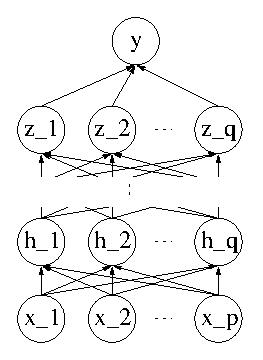
\includegraphics[width=0.75\columnwidth]{figures/mlp.eps}
    \end{minipage}
    \begin{minipage}{0.48\textwidth}
        \centering
        \psfrag{x_1}[Cc][Cc][1][0]{$x_1$}
        \psfrag{x_2}[Cc][Cc][1][0]{$x_2$}
        \psfrag{x_p}[Cc][Cc][1][0]{$x_p$}
        \psfrag{h_1}[Cc][Cc][1][0]{$h^{\qlay{1}}_1$}
        \psfrag{h_2}[Cc][Cc][1][0]{$h^{\qlay{1}}_2$}
        \psfrag{h_q}[Cc][Cc][1][0]{$h^{\qlay{1}}_{q_1}$}
        \psfrag{z_1}[Cc][Cc][1][0]{$h^{\qlay{L}}_1$}
        \psfrag{z_2}[Cc][Cc][1][0]{$h^{\qlay{L}}_2$}
        \psfrag{z_q}[Cc][Cc][1][0]{$h^{\qlay{L}}_{q_L}$}
        \psfrag{y}[Cc][Cc][1][0]{$\vy$}
        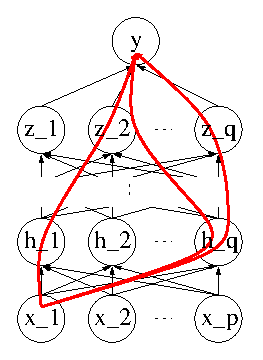
\includegraphics[width=0.75\columnwidth]{figures/mlp_multicomp.eps}
    \end{minipage}

    \vspace{2mm}
    \begin{minipage}{0.48\textwidth}
        \centering
        \small
        (a) Multi-layer Perceptron
    \end{minipage}
    \begin{minipage}{0.48\textwidth}
        \centering
        \small
        (b) Multiple Computational Paths
    \end{minipage}
    \caption{Illustrations of (a) a multi-layer perceptron
    and (b) an example of multiple computational paths
    starting from $x_1$ to $\vy$. In (b), the red arrows
    illustrate three different paths sharing hidden units.}
    \label{fig:mlp}
\end{figure}

An MLP can approximate a nonlinear function
$f$ in Eq.~\eqref{eq:linreg_gen} with a set $D$ of training
samples. Assuming linear output units (see
Eq.~\eqref{eq:linear_unit}), the output of an MLP with $L$
intermediate hidden layers is
\begin{align*}
    u(\vx) = \mU^\top \phi_{\qlay{L}} \left(
    \mW_{\qlay{L}}^\top \phi_{\qlay{L-1}} \left(
    \mW_{\qlay{L-1}}^\top \cdots \phi_{\qlay{1}} \left( \mW_{\qlay{1}}^\top \vx \right)
    \cdots \right) \right),
\end{align*}
where $\mU$ and $\mW_{\qlay{l}}$ are the weights of the
edges between the $L$-th intermediate layer and the output
layer and between $(l-1)$-th and $l$-th layers,
respectively.  $\phi_{\qlay{l}}$ is a component-wise
nonlinear function at the $l$-th layer, such as the sigmoid
function in Eq.~\eqref{eq:sigmoid}.  We have omitted biases
for notational simplicity.

This can be re-written by considering each intermediate
hidden layer $l$ as a nonlinear module $g_{\qlay{l}}$ such that
\begin{align*}
    g_{\qlay{l}}(\vx) = \phi_{\qlay{l}}(W_{\qlay{l}}^\top \vx),
\end{align*}
and
\begin{align*}
    u(\vx) = \mU^\top 
    \left(g_{\qlay{L}} \circ g_{\qlay{L-1}} \circ \cdots
    \circ g_{\qlay{1}} (\vx) \right).
\end{align*}
In this way, we can say that the MLP is a composition of
multiple layers of nonlinear modules \citep{Bengio2007a}.

Each intermediate nonlinear layer transforms the coordinate
of the input from the layer below nonlinearly. For instance,
the vector of hidden activations one layer below
$\vh_{\qlay{l-1}} \in \left[ 0, 1\right]^p$ is transformed into
$\vh_{\qlay{l}} \in \left[0, 1\right]^q$, if the sigmoid nonlinear
activation function is used. Therefore, if we consider the
composition compositeof the intermediate layers as a single nonlinear
transformation, it can be said that the top layer performs a
\textit{linear} regression, or classification, on the
nonlinearly transformed dataset. 
%It should be emphasized that each layer
%is \textit{trainable} in a sense that we learn the
%corresponding weights according to the given training set.

Another way to look at what each intermediate layer does is
to consider it as a \textit{feature detector} \citep[see,
e.g.,][]{Haykin2009}. The $j$-th hidden unit $h_j^{\qlay{l}}$ in
the $l$-th intermediate layer is likely to be active, if the
activation in the layer immediately below embeds a feature
similar to the associated weights $\left[ w_{1,j}^{\qlay{l}},
\cdots, w_{p,j}^{\qlay{l}} \right]$, where $p$ is the number of
units in the layer below. In other words, each unit detects
a feature in the activation of the layer below.

It is obvious that there exists more than one computational
path from an input vector to a unit in any intermediate
layer $l$ ($l > 1$), assuming that there are more than one
intermediate layers each consisting of more than one hidden
units and most of the weights parameters are not zero. This
implies that each intermediate unit \textit{shares} the
features detected by the units in the lower (closer to the
input layer) layers.  See Fig.~\ref{fig:mlp}(b) for an
illustration.

Each intermediate layer is \textit{trainable} in the sense
that the associated parameters are fitted to a given
training set $D$ by minimizing the following joint cost
function:
\begin{align}
    \label{eq:mlp_cost}
    J(\TT) = \sum_{n=1}^N d\left(y^{(n)}, u(\vx^{(n)})\right),
\end{align}
where $d(\cdot, \cdot)$ is a suitably chosen distance
function. For a regression task, the Euclidean distance may be
used, as in Eq.~\eqref{eq:linreg_cost}, and for a
classification task, one may use the cross-entropy loss, as in
Eq.~\eqref{eq:crossentropy_cost}. Learning the parameters of
multiple layers can be efficiently done by the backpropagation
algorithm \citep{Rumelhart1986}, which will be discussed more
in Section~\ref{sec:backprop}.

The importance of having one or more intermediate layers of
nonlinear hidden units between the input and output units
has been highlighted by the universal approximator property
\citep{Cybenko1989,Hornik1989}. It basically states that
there exists an MLP with a single hidden layer that can
approximate a continuous function whose support is on a
hypercube, with an arbitrary small error.

%An MLP is sometimes referred to as a feedforward neural
%network, as signal propagates in a single direction starting
%from the input units toward the output units. There is no
%recurrent edge that enables a signal begun from the input
%unit to reach a unit more than once. In terms of graphical
%models, an MLP is a directed \textit{acyclic} graph
%\citep{Bondy2008}.

This model is a typical example of a deep neural network
that can be characterized by having \textit{multiple layers
of trainable feedforward nonlinear hidden units}. This
model trivially satisfies the two conditions for being a
deep neural network.

\subsection{Related, but Shallow Neural Networks}

Here we explain some models that are closely related to an
MLP, but are not considered deep.

\subsubsection{Support Vector Machines and Kernel Methods}
\label{sec:svm}

A support vector machine (SVM\nomenclature{SVM}{Support vector
machine}) proposed by
\citet{Cortes1995} is one of the most widely used neural
network models. The SVM is based on two important ideas
which are the maximum-margin principle and kernel methods.
We briefly describe these principles and try to find the
connection to the MLP here.  For more details on SVMs, the
readers are referred to \citep{Scholkopf2001}.

The maximum-margin principle provides a principled way of
regularizing the parameters of a model. For instance, in the
case of a classifier separating two classes (see
Section~\ref{sec:perceptron}), the optimal separating
hyperplane is the one that has the maximal margin of separation,
where the margin of separation is the distance between the
hyperplane and the closest training samples from both
classes.

Under this principle, the objective of training a
perceptron, assuming $-1$ and $1$ as the outputs of the
Heaviside function in Eq.~\eqref{eq:heaviside_func} and each
output $y^{(n)} \in \{ -1, 1 \}$, becomes
\begin{align}
    \label{eq:svm_primal}
    &\min \frac{1}{2} \| \vw \|^2
\end{align}
subject to
\begin{align*}
    &y^{(n)} \left( \vw^\top \vx^{(n)} + b \right) \geq 1,
    \forall n = 1, \dots , N
\end{align*}
Once the optimization is over, the separating hyperplane
with the maximum margin can be mathematically described in
terms of support vectors, as in Fig.~\ref{fig:svm}(a).

A kernel method 
%employed by an SVM 
for an SVM
does a similar thing to
what the intermediate hidden layers of an MLP do. Instead of
training a linear classifier directly on raw training
samples, consider training a classifier on, possibly
nonlinearly, transformed samples. Let us denote the
nonlinear vector transformation $\phi$. Then, in essence,
the classifier is trained not on $D = \left\{ \left(
\vx^{(n)}, y^{(n)} \right) \right\}_{n=1}^N$, but on
$\tilde{D} = \left\{ \left( \phi(\vx^{(n)}), y^{(n)} \right)
\right\}$. It is easy to see the connection to MLPs
explained earlier by comparing $\phi$ to the multiple
intermediate layers of hidden units.

However, instead of using an explicit transformation $\phi$,
the kernel method uses a \textit{kernel} function $k(\cdot,
\cdot)$ between two samples. This is justified by looking at
a dual form of the objective function in
Eq.~\eqref{eq:svm_primal} obtained by introducing Lagrangian
multipliers $\valpha$.  In a dual form, the output $y$ of an
unseen, test sample $\vx$ is written as
\begin{align*}
    y = \phi \left( \sum_{n=1}^N \alpha_n y^{(n)}
    {\vx^{(n)}}^\top \vx + b \right),
\end{align*}
where $\phi$ is the Heaviside function,
and we may replace the inner product between $\vx^{(n)}$ and
$\vx$  with a positive-definite kernel function
$k(\vx^{(n)}, \vx)$.

In fact, it is possible to build an equivalent MLP when a
certain type of kernel function is used. For instance, an
MLP equivalent to the SVM with the hyperbolic tangent kernel
function (see Eq.~\eqref{eq:tanh})
\begin{align*}
    k(\vx, \vx') = \tanh(\beta_0 \vx^\top \vx' + \beta_1)
\end{align*}
can be constructed.
%\citep[see, e.g.,][]{Haykin2009}. 

An equivalent, but not necessarily optimal, MLP has a
single intermediate hidden layer with $N$ hidden units, each
having a hyperbolic tangent activation function. The weights
$\mW$ of the edges connecting the input units to the hidden
units are fixed to the training samples scaled by $\beta_0$,
that is, $\mW = \beta_0 \left[ \vx^{(1)}, \vx^{(2)}, \cdots,
\vx^{(N)} \right]$. The biases to all the hidden units are
set to $\beta_1$. The weights of outgoing edges from the
hidden units to the output unit are $\mU = \left[ \alpha_1 y^{(1)}, \alpha_2 y^{(2)}, \cdots, \alpha_N y^{(N)}
\right]^\top$, and the bias to the output unit is $b$. The
structure of this MLP is illustrated in
Fig.~\ref{fig:svm}(b).

\begin{figure}[t]
    \begin{minipage}{0.48\textwidth}
        \centering
        \psfrag{y=1}[Cc][Cr][1][0]{$y=1$}
        \psfrag{y=0}[Cc][Cr][1][0]{$y=0$}
        \psfrag{y=-1}[Cc][Cr][1][0]{$y=-1$}
        \psfrag{Margin}[Cc][Cc][1][0]{Margin}
        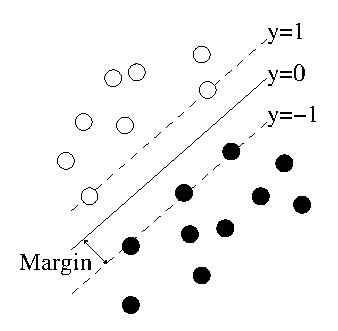
\includegraphics[width=0.75\columnwidth]{figures/svm_maxmargin.eps}
    \end{minipage}
    \begin{minipage}{0.48\textwidth}
        \centering
        \psfrag{x_1}[Bc][Bc][1][0]{$x_1$}
        \psfrag{x_2}[Bc][Bc][1][0]{$x_2$}
        \psfrag{x_p}[Bc][Bc][1][0]{$x_p$}
        \psfrag{v_1}[Bc][Bc][0.8][0]{$\beta_0 \vx^{(1)}$}
        \psfrag{v_2}[Bc][Bc][0.8][0]{$\beta_0 \vx^{(2)}$}
        \psfrag{v_N}[Bc][Bc][0.8][0]{$\beta_0 \vx^{(N)}$}
        \psfrag{h_1}[Bc][Bc][1][0]{$h_1$}
        \psfrag{h_2}[Bc][Bc][1][0]{$h_2$}
        \psfrag{h_N}[Bc][Bc][1][0]{$h_N$}
        \psfrag{a_1}[Bc][Bc][0.8][0]{$\alpha_1 y^{(1)}$}
        \psfrag{a_2}[Bc][Bc][0.8][0]{$\alpha_2 y^{(2)}$}
        \psfrag{a_N}[Bc][Bc][0.8][0]{$\alpha_N y^{(N)}$}
        \psfrag{y}[Bc][Bc][1][0]{$y$}
        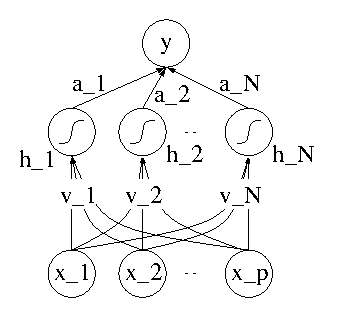
\includegraphics[width=0.75\columnwidth]{figures/mlp_svm.eps}
    \end{minipage}

    \vspace{2mm}
    \begin{minipage}{0.48\textwidth}
        \centering
        \small
        (a) Maximum Margin
    \end{minipage}
    \begin{minipage}{0.48\textwidth}
        \centering
        \small
        (b) Equivalent MLP
    \end{minipage}
    \caption{Illustrations of (a) the maximum-margin
    principle and (b) constructing a multi-layer
    perceptron equivalent to a given support vector machine.
    In (a), there are two classes (denoted by black and
    white circles). A solid line is the maximum-margin
    separating hyperplane, and the samples on the dashed
    lines are support vectors. In (b), it should be noticed
    that this construction is \textit{not} optimal, as any
    hidden unit not corresponding to a support-vector may be
    omitted.}
    \label{fig:svm}
\end{figure}

%This way of building an equivalent MLP is possible for
%many kernel functions. Only difference
%from the previous description of an MLP is that the
%nonlinear function used in the hidden units is not
%necessarily bounded from either up or down.

It suggests that a kernel method is one way to extend the
simple, linear neural network by adding one intermediate
nonlinear hidden layer. However, this is often considered a
\textit{shallow} neural network, since the number of
intermediate hidden layers is limited to one, and the added
layer is usually \textit{not} trainable \citep{Bengio2007a}.
Because there is only a single intermediate layer, there is
no sharing of features detected in the lower layers.
Essentially, a kernel method is a principled way to apply a
template-matching approach to a machine learning problem.

We do not consider nor discuss kernel methods, as
well as SVMs, any further in this thesis.  It should be,
however, noted that there has been a few attempts to make it
deeper recently by \citet{Cho2009} and \citet{Damianou2012}.
Also, there has been a study linking the maximum-margin
principle used in SVMs to a learning criterion of
multi-layer perceptrons as well as a simpler perceptron
\citep[see, e.g.,][]{Collobert2004}.

\subsubsection{Extreme Learning Machines}
\label{sec:elm}

Another related model is an extreme learning machine
(ELM\nomenclature{ELM}{Extreme learning machine}) proposed
recently by \citet{Huang2006}. The ELM is, in essence, an
MLP with a \textit{single} intermediate layer of nonlinear
hidden units.

The main difference between an ELM and an MLP is whether all
layers are jointly adapted to minimize the cost function in
Eq.~\eqref{eq:mlp_cost}. While the parameters of all layers
of an MLP are jointly estimated, in an ELM, only the
parameters of the last output layer or the outgoing weights
from the penultimate layer to the output layer, are
adapted\footnote{
A similar idea of learning only the parameters of the last
output layer has also been proposed and used for
recurrent neural networks \citep[see, e.g.,][]{Jaeger2009}.
}.

This is equivalent to using shallow supervised neural
networks, presented in Section~\ref{sec:supervised_model}
with a transformed training set $\tilde{D}=\left\{ \left(
\phi(\vx^{(n)}), y^{(n)} \right) \right\}$. The
transformation $\phi(\vx)$ corresponds to the activations of
the intermediate layer.  Interestingly, in an ELM, the
parameters of the transformation $\phi$ are not estimated,
but \textit{sampled} from a random distribution.
%, usually, zero-mean Gaussian distribution.

One of the underlying reasons why an ELM \textit{works} at
all is the Cover's separability theorem
\citep{Cover1965}
%,Haykin2009} 
stating that samples in a
classification problem are more likely to become linearly
separable when the input is nonlinearly transformed to a
higher-dimensional space. Under this theorem, an ELM can be
considered as a two-step model that first nonlinearly
projects an input sample $\vx$ into a higher-dimensional
space $\phi(\vx)$ ($q > p$) to make it, in probability, more
likely to be linearly separable and then performs
classification/regression in the new space.

Since it is relatively easy and computationally efficient to
estimate the parameters of the shallow neural networks, the
most obvious advantage of using an ELM over an MLP is
\textit{speed}. Furthermore, the cost function then
becomes a convex function, which prevents any problem
arising from the existence of many, potentially infinite
local minima, again unlike an MLP. These reasons have led
to the popularity of ELM recently \citep{Huang2011}.

Similarly to the SVM we discussed right before, an ELM is
not a deep neural network.  Firstly, it
is not clear whether stacking any more intermediate layers
with randomly sampled parameters would improve the
performance.  If we naively consider the Cover's theorem,
there is no theoretical or empirical motivation for using
multiple layers of gradually increasing dimensionality
compared to just using a large number of hidden units in a
single intermediate layer.  Thus, it does not satisfy the
first condition.  Secondly, the parameters between the input
and intermediate hidden layers are \textit{not} trained,
further violating the second condition.


\section{Deep Autoencoders}
\label{sec:autoencoders}

As was the case with MLPs, a linear autoencoder can have
more modeling power by employing multiple nonlinear
intermediate layers symmetrically in the encoder and
decoder. The units corresponding to the hidden variables in
Eq.~\eqref{eq:lvm} may also be replaced with nonlinear units
instead of the linear units originally used in the linear
autoencoder. We call this a \textit{deep} autoencoder, and
it is a typical example of an unsupervised deep neural
network.

\begin{figure}[t]
    \centering
    \psfrag{x_1}[Bc][Bc][1.2][0]{$x_1$}
    \psfrag{x_2}[Bc][Bc][1.2][0]{$x_2$}
    \psfrag{x_p}[Bc][Bc][1.2][0]{$x_p$}
    \psfrag{y_1}[Bc][Bc][1.2][0]{$\tilde{x}_1$}
    \psfrag{y_2}[Bc][Bc][1.2][0]{$\tilde{x}_2$}
    \psfrag{y_p}[Bc][Bc][1.2][0]{$\tilde{x}_p$}
    \psfrag{u_1}[Bc][Bc][1.2][0]{$h_1$}
    \psfrag{u_q}[Bc][Bc][1.2][0]{$h_q$}
    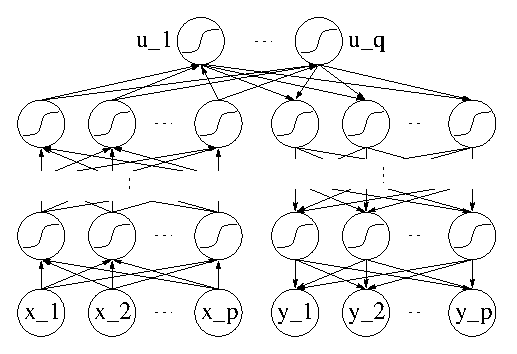
\includegraphics[width=0.75\columnwidth]{figures/deepae.eps}
    \caption{Illustration of a deep autoencoder. The
    left- and right- halves correspond to the encoder and
    decoder, respectively. Although each hidden node is
    drawn to have a sigmoid nonlinear activation function,
    a different activation function may be used.}
    \label{fig:dae}
\end{figure}

When there are $L-1$ intermediate layers of hidden units,
both in the encoder and decoder, the encoder becomes
\begin{align}
    \label{eq:ae_encoder}
    \vh = f(\vx) = f_{
    \qlay{L-1}} \circ f_{\qlay{L-2}} \circ \cdots \circ
    f_{\qlay{1}}(\vx)
\end{align}
and the decoder is
\begin{align}
    \label{eq:ae_decoder}
    \tilde{\vx} = g(\vx) = g_{\qlay{1}} \circ g_{\qlay{2}} \circ \cdots \circ
    g_{\qlay{L-1}} (\vh),
\end{align}
where $f_{\qlay{l}}$ and $g_{\qlay{l}}$ are the encoding and decoding
nonlinear modules at the $l$-th layer. They are
defined by
\begin{align*}
    f_{\qlay{l}}(\vs_{\qlay{l-1}}) = \phi_{\qlay{l}}
    \left(\mW_{\qlay{l}}^\top \vs_{\qlay{l-1}} +
    \vb_{\qlay{l}}\right)
\end{align*}
and
\begin{align*}
    g_{\qlay{l}}(\vs_{\qlay{l+1}}) = \varphi_{\qlay{l}}
    \left(\mU_{\qlay{l}} \vs_{\qlay{l+1}} + \vc_{\qlay{l}}
    \right),
\end{align*}
where $\mW_{\qlay{l}}$, $\mU_{\qlay{l}}$, $\vb_{\qlay{l}}$
and $\vc_{\qlay{l}}$ are parameters
of the $l$-th hidden module, and $\phi_{\qlay{l}}$ and
$\varphi_{\qlay{l}}$
are component-wise nonlinearities used in the encoder and
decoder, respectively.  $f$ here should not be confused with
the unknown generating function $f$ in Eq.~\eqref{eq:lvm}.
We may simply write $f = f_{\qlay{L-1}} \circ \cdots \circ
f_{\qlay{1}}$ and
$g = g_{\qlay{1}} \circ \cdots \circ g_{\qlay{L-1}}$. See Fig.~\ref{fig:dae}
for the illustration.

The parameters of a deep autoencoder can be found by
minimizing the difference between the original input
$\vx^{(n)}$ and the reconstructed input $\tilde{\vx}^{(n)}$
for all $N$ training samples, as in
Eq.~\eqref{eq:autoencoder_cost}. Of course, the difference
may be measured by any suitable distance metric such as, for
instance, a squared Euclidean distance or a cross-entropy
loss in the case of binary inputs.

We may call this a \textit{deep} autoencoder, as this
network satisfies the conditions of being a deep neural
network. The network can be further extended by employing
more intermediate hidden layers, and each and every layer is
trainable.

This way of extending a linear autoencoder by adding
multiple intermediate layers of hidden units with a
bottleneck layer has been proposed by, for instance,
\citet{Oja1991} and \citet{Kramer1991}. In these early
works, it was usual to use a bottleneck layer with less
units to perform 
dimensionality reduction or data compression.

\subsection{Recognition and Generation}
\label{sec:autoencoder_prob}

A deep autoencoder is nothing but a plain MLP if we
transformed a training set $D$ consisting of only inputs 
\[
D = \left\{ \vx^{(1)}, \dots, \vx^{(N)} \right\}
\]
to another training set $\tilde{D}$ such that the label of
each training sample is the training sample itself:
\[
\tilde{D} = \left\{ \left( \vx^{(1)}, \vx^{(1)}\right),
\dots, \left( \vx^{(N)}, \vx^{(N)}\right) \right\}.
\]
However, it becomes more interesting when we look at the
deep autoencoder as a sequential composition of recognition
and generation of a set of visible units.

Let us restate the underlying unsupervised model in
Eq.~\eqref{eq:lvm}:
\begin{align*}
    \vx = g(\vh) + \epsilon.
\end{align*}
This model specifies the generation of each sample $\vx$
given the corresponding latent representation. If we further
constraint the model to be explicitly parameterized, we get 
\begin{align*}
    \vx  = g(\vh \mid \TT_g) + \epsilon,
\end{align*}
where $\TT_g$ is a set of parameters. Furthermore, let us
assume that $\vx$ and $\vh$ are binary vectors such that
each component of them is either $0$ or $1$. Instead of $f$
in the original equation \eqref{eq:lvm}, we used $g$ for
making the connection with the autoencoder more clearly.

In this section, we consider a probabilistic perspective from
which a deep autoencoder can be viewed. From this
perspective, we assume that the training samples were
generated from the set of latent variables in a bottleneck
layer. Then, the encoder is expected to approximately infer
the states of the latent variables given a sample in the
visible layer, and the decoder to generate a sample from the
inferred latent variables.

\subsection{Variational Lower Bound and Autoencoder}
\label{sec:autoencoder_vari}

Since we will now view this model in a probabilistic
framework, let us define a prior distribution over $\vh$
with the
Bernoulli distribution, with parameterized probability masses
$\gamma$ and $1-\gamma$ :
\begin{align}
    \label{eq:ae_prior}
    p(\vh) = \prod_{j=1}^q \gamma^{h_j} (1 - \gamma)^{1 -
    h_j}
\end{align}
We assume now that there exists a parameterized
deterministic nonlinear mapping $g$ from $\vh$ to $\vx$ such
that the conditional distribution of $\vx$ given $\vh$ is
\begin{align}
    \label{eq:ae_cond}
    p(\vx \mid \vh) = \prod_{i=1}^p \tilde{x}_i^{x_i} (1 -
    \tilde{x}_i)^{1 - x_i},
\end{align}
where $\tilde{\vx} = g(\vh \mid \TT_g)$. These fully
describe the probabilistic model 
\begin{align}
    \label{eq:ae_full}
p(\vx, \vh \mid \TT_g) = p(\vx \mid \vh) p(\vh).
\end{align}

Let us further assume that there is a deterministic
nonlinear mapping $f$, parameterized by $\TT_f$ that
approximates the factorized posterior distribution over
$\vh$ given $\vx$:
\begin{align}
    \label{eq:ae_posterior}
    Q(\vh) = \prod_{j=1}^q q(h_j),
\end{align}
where $\vmu = f(\vx \mid \TT_f)$ and $q(h_j = 1) = \mu_j$.
For now, we assume that $\TT_f$ is fixed.

Since the exact evaluation of the marginal log-likelihood is
intractable, the parameters $\TT_g$ of the decoder then
can be found by maximizing the lower bound of the marginal
log-likelihood $\log p(D = \left\{ \vx^{(n)}
\right\}_{n=1}^N \mid \TT_g)$:
\begin{align*}
    \log p(D \mid \TT_g) \geq \E_{Q(\vh)} \left[ \log p\left(D,
    H=\left\{ \vh^{(n)} \right\}_{n=1}^N \mid \TT_g\right) \right] +
    \text{const},
\end{align*}
where 
\begin{align*}
    \log p(D, H \mid \TT_g) = \sum_{n=1}^N \sum_{i=1}^p
    x^{(n)}_i \log
    \tilde{x}^{(n)}_i + (1 - x^{(n)}_i) \log (1 -
    \tilde{x}^{(n)}_i) + \text{const}.
\end{align*}
and the equality holds only when $Q(\vh)$ is the true
posterior distribution. See Section~\ref{sec:ppca} to see
how the lower bound is derived.

It is easy to see that this corresponds to learning the
parameters of the decoder of an autoencoder by minimizing
the cross-entropy loss in Eq.~\eqref{eq:crossentropy_cost}.
The only difference is that the bottleneck layer consists of
stochastic units where their activations are sampled
rather than decided deterministically. 

This suggests that the decoder $g$ of the deep autoencoder
(see Eq.~\eqref{eq:ae_decoder}) \textit{generates} a visible
sample starting from its latent representation, following
the model given in Eq.~\eqref{eq:ae_full}. On the other
hand, the encoder $f$ \textit{recognizes} a visible sample
by encoding it into a latent representation, which is in the
probabilistic framework equivalent to inferring the
posterior distribution over the latent variables $\vh$.
However, it should be understood that the encoder $f$ does
not perform exact inference, but only approximate inference
assuming the fully factorized posterior distribution $Q$ in
Eq.~\eqref{eq:ae_posterior}, without trying to reduce
the Kullback-Leibler divergence between $Q$ and the true
posterior distribution.

If we drop the binary constraint of $\vx$ and instead assume
that $\vx$ follows a multi-variate Gaussian distribution
with a diagonal covariance matrix, we get the marginal
log-likelihood that corresponds to the negative sum of
squared reconstruction error (see
Eq.~\eqref{eq:autoencoder_cost}).

However, this interpretation does neither provide an
intuitive way of learning the parameters $\TT_f$ of the
encoder $f$ nor tell us how latent representations should be
designed.  \citet{Vincent2010} argued that minimizing the
reconstruction error in an autoencoder trained by, for
instance, backpropagation is equivalent to maximizing the
lower bound of the mutual information between the input
$\vx$ and latent representation $\vh$. 
%A wake-sleep algorithm, which will
%be discussed in more detail later, proposed by
%\citet{Hinton1995} learns $\TT_f$, and $\TT_g$ together, by
%the principle of minimum description length \citep[see,
%e.g.,][and references therein]{Grunwald2007}.

Combining these two approaches, in summary a deep
autoencoder \textit{recognizes} an input sample $\vx$ with a
latent representation $\vh$ such that the mutual information
between them is maximal, and \textit{generates} a
reconstructed sample $\tilde{\vx}$ from the latent
representation $\vh$ so that the reconstruction error
between the original input $\vx$ and the reconstructed
sample $\tilde{\vx}$ is minimal.

%\subsubsection{Combinations with and Connections to Other
%Approaches}

\subsection{Sigmoid Belief Network and Stochastic Autoencoder}
\label{sec:sbn_dbn}

A sigmoid belief network, proposed by \citet{Neal1992},
consists of a single layer of stochastic binary visible
units $\vx$ and $L > 0$ layers of stochastic binary
hidden units $\vh^{\qlay{l}}$ such that a sample $\vx$ is
generated starting from the activations of the $L$-th layer
hidden units sampled from
\[
p\left(h_j^{\qlay{L}} = 1\right) = \phi\left( b_j^{\qlay{L}}
\right)
\]
by iteratively sampling from 
\begin{align}
    \label{eq:sbn_gen_h}
    p\left(h_j^{\qlay{l}} = 1 \left| h_1^{\qlay{l+1}},
    h_2^{\qlay{l+1}}, \dots
    \right.\right) = \phi\left( \sum_{k} w_{jk}^{\qlay{l}}
    h_k^{\qlay{l+1}} + b_j^{\qlay{l}}\right),
\end{align}
where $\phi$ is a sigmoid function (see
Eq.~\eqref{eq:sigmoid}). 

Obviously, the probability of each component $x_i$ given the
activations of the units in the layer above is
\begin{align}
    \label{eq:sbn_gen_x}
    p\left(x_i = 1 \left| \vh^{\qlay{1}}
    \right.\right) = \phi\left( \sum_{j} w_{ij}
    h_j^{\qlay{1}} + b_j\right).
\end{align}
Note that this description assumes that there are no
intra-layer edges. This is not necessary, but makes it much
easier to understand the generative process the network is
modeling.

Once the sigmoid belief network has been trained, one 
important task is to \textit{infer} the states of the hidden
units given a novel sample. However, it is not trivial to do
so due to the nonlinear nature of multiple layers of the
hidden units.

\citet{Hinton1995} proposed a wake-sleep algorithm, which is
based on the principle of minimum description length
%\citep[see, e.g.,][and references therein]{Grunwald2007},
\citep{Rissanen1978},
that learns simultaneously the \textit{generative}
parameters $\TT_+$, used in
Eqs.~\eqref{eq:sbn_gen_h}--\eqref{eq:sbn_gen_x}, and the
\textit{recognition} parameters $\TT_-$, used for
approximate inference of the posterior distribution over the
hidden units. Since it is intractable to compute the
posterior distribution exactly, the wake-sleep algorithm
instead maximizes the lower bound $\LL_Q(\TT)$ of the true
marginal log-likelihood $\LL(\TT) = \sum_{n=1}^N \log
\sum_{\vh} p(\vx^{(n)}, \vh \mid \TT)$ (see
Eqs.~\eqref{eq:mll_decom}--\eqref{eq:kldiv}).

Let us look at a single update step given a single data
sample $\vx$.  In the \textit{wake} stage, samples of the
hidden units are collected from the approximate posterior
distribution $Q$ parameterized by the recognition parameters
$\TT_-$. With the fixed samples $h^{\qlay{l}}_j$'s from all the
hidden layers, the conditional expectation $p^{\qlay{l}}_j$ of
each hidden unit is computed using Eq.~\eqref{eq:sbn_gen_h}
with the generative parameters $\TT_+$. Then, we update each
generative weight $w_{ij}^{\qlay{l}}$ by
\begin{align}
    \label{eq:sbn_wake}
    w_{ij}^{\qlay{l}} \leftarrow w_{ij}^{\qlay{l}} + \eta
    (h^{\qlay{l}}_i -
    p^{\qlay{l}}_i) h^{\qlay{l+1}}_j.
\end{align}

In the \textit{sleep} stage, the process is reversed.
Samples of the hidden units are collected starting from the
top layer in a top-down manner using the generative
parameters $\TT_+$. This time, the conditional expectation
$p^{(l)}_j$ is computed using the recognition parameters
$\TT_-$. With these, each recognition weight $u_{ij}^{(l)}$
is updated by
\begin{align}
    \label{eq:sbn_sleep}
    u_{ij}^{(l)} \leftarrow u_{ij}^{(l)} + \eta s^{(l)}_i
    (s^{(l+1)}_j - p^{(l+1)}_k).
\end{align}

\begin{figure}[t]
    \centering
    \psfrag{x_1}[Bc][Bc][1][0]{$x_1$}
    \psfrag{x_p}[Bc][Bc][1][0]{$x_p$}
    \psfrag{h_1}[Bc][Bc][1][0]{$h^{(1)}_1$}
    \psfrag{h_q}[Bc][Bc][1][0]{$h^{(1)}_q$}
    \psfrag{z_2}[Bc][Bc][1][0]{$h^{(2)}_j$}
    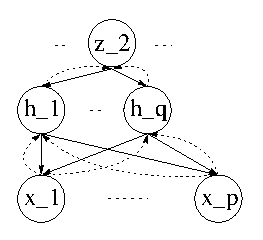
\includegraphics[width=0.4\columnwidth]{figures/sbn.eps}
    \caption{Illustration of a sigmoid belief network having
    two hidden layers.  The solid lines indicate the
    generation path starting from the top hidden layer and
    are parameterized by the generation parameters. The
    dashed curves correspond to the recognition paths starting
    from the bottom, visible layer, parameterized by the
    recognition parameters.}
    \label{fig:sbn}
\end{figure}

It is easy to spot the similarity between the deep
autoencoder and the sigmoid belief network trained with the
wake-sleep algorithm (see Fig.~\ref{fig:sbn} for an
example). Both of them maintain two sets of parameters;
encoding and decoding parameters of the autoencoder, and
recognition and generation parameters of the sigmoid belief
network. The encoder and the recognition parameters are
used to \textit{infer} the states of the hidden units given
a sample. The decoder and the generative parameters
\textit{generate} a sample given the states of the hidden
units.

However, unlike the encoder in the autoencoder which
computes the activation of each hidden unit
\textit{deterministically}, the recognition of the sigmoid
belief network computes the activation \textit{probability}
of each hidden unit. An actual activation needs to be
sampled. The same difference exists in the process of
generation. Hence, we may consider the recognition and
generation passes of the sigmoid belief network as a
\textit{stochastic} deep autoencoder, however, trained with an
objective function other than the reconstruction error.
We will discuss more this difference in connection to
the up-down algorithm proposed to train a deep belief
network \citep{Hinton2006nc} later in
Section~\ref{sec:det_vs_sto}.

A deep belief network (DBN\nomenclature{DBN}{Deep belief
network}) \citep{Hinton2006nc} extends the
sigmoid belief network by adding a layer of undirected
network on its top. For the remaining lower layers, the DBN
keeps, as did the sigmoid belief network, two separate sets
of parameters; recognition and generative parameters
\citep{Hinton2006nc}.  Except for the top two layers which
are connected with undirected edges, it is clear that the
encoder and decoder of a deep autoencoder correspond to the
deterministic version of the recognition and generation
weights of the DBN.

More on the deep belief network will be presented in
Section~\ref{sec:dbn}.

\subsection{Gaussian Process Latent Variable Model}

Under this probabilistic approach, it is possible to use
only a
part of a deep autoencoder together with another
probabilistic model. For instance, any latent variable model
may use the encoder of a deep autoencoder to perform a fast
inference of hidden variables. Here, we will briefly
describe one such model, called a Gaussian process latent
variable model with back-constraints.

The Gaussian process latent variable model
(GP-LVM\nomenclature{GP-LVM}{Gaussian process latent variable
model}) proposed
by \citet{Lawrence2003} is a dual formulation of
probabilistic PCA introduced earlier in
Section~\ref{sec:ppca}.  Whereas the probabilistic PCA tries
to maximize the log-likelihood with respect to the weights
after marginalizing out the hidden variables $\vh$, the basic
version of GP-LVM maximizes the log-likelihood with respect
to the hidden variables and hyper-parameters after
marginalizing out the weights.

Instead of putting a prior distribution over $\vh$, GP-LVM
puts a prior distribution over $\mW$ such that
\begin{align*}
    p(\mW) = \prod_{i=1}^p \N(\vw_i \mid \vzero, \alpha^{-1}
    \mI),
\end{align*}
where $\NN(\vw \mid \vm, \mS)$ is a probability density of
$\vx$ under a multivariate Gaussian distribution with mean
$\vm$ and covariance $\mS$. Then, the marginal
log-likelihood, after marginalizing out the weights, becomes
\begin{align}
    \label{eq:gplvm_mll}
    \LL = -\frac{qN}{2} \log 2\pi - \frac{q}{2} \log \left|
    \mK \right| - \frac{1}{2}\text{tr}(\mK^{-1} \mX \mX^\top),
\end{align}
where $\mH = \left[ \vh^{(1)}, \dots, \vh^{(N)}
\right]^\top$ and $\mK = \alpha \mH \mH^\top + \sigma^2
\mI$. The illustration of this probabilistic model is shown
in Fig.~\ref{fig:gplvm}(a). It is usual to replace $\mH
\mH^\top$ in $\mK$ with a nonlinear kernel matrix with
hyper-parameters to construct a nonlinear GP-LVM. However,
unless the linear kernel matrix is used, it is difficult to
find an analytical solution for both the hyper-parameters
and the hidden representations, and one must resort to an
iterative optimization algorithm.

\begin{figure}[t]
    \begin{minipage}{0.48\textwidth}
        \centering
        \psfrag{x_n}[Bc][Bc][1][0]{$\vx^{(n)}$}
        \psfrag{h_n}[Cc][Cc][1][0]{$\vh^{(n)}$}
        \psfrag{s}[Cc][Cc][1][0]{$\sigma^2$}
        \psfrag{N}[Cc][Cc][1][0]{$N$}
        \psfrag{W}[Cc][Cc][1][0]{$\mW$}
        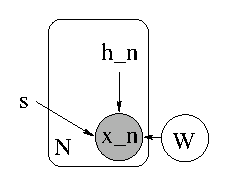
\includegraphics[width=0.65\columnwidth]{figures/gplvm.eps}
    \end{minipage}
    \begin{minipage}{0.48\textwidth}
        \centering
        \psfrag{x_n}[Bc][Bc][1][0]{$\vx^{(n)}$}
        \psfrag{h_n}[Cc][Cc][1][0]{$\vh^{(n)}$}
        \psfrag{s}[Cc][Cc][1][0]{$\sigma^2$}
        \psfrag{N}[Cc][Cc][1][0]{$N$}
        \psfrag{W}[Cc][Cc][1][0]{$\mW$}
        \psfrag{h_1}[Cc][Cc][1][0]{$\vh_1$}
        \psfrag{h_2}[Cc][Cc][1][0]{$\vh_2$}
        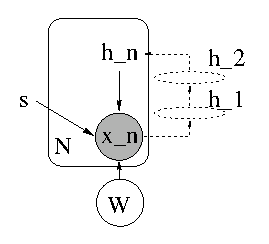
\includegraphics[width=0.8\columnwidth]{figures/gplvm_bc.eps}
    \end{minipage}

    \vspace{2mm}
    \begin{minipage}{0.48\textwidth}
        \centering
        \small
        (a) GP-LVM
    \end{minipage}
    \begin{minipage}{0.48\textwidth}
        \centering
        \small
        (b) With Back-Constraint
    \end{minipage}
    \caption{Illustrations of a Gaussian process
    latent-variable model (a) with and (b) without
    back-constraint. Note that the differences from the
    probabilistic principal component in
    Fig.~\ref{fig:naive_bayes}(b) that in GP-LVM,
    $\vh^{(n)}$ is \textit{not} a random variable whereas
    $\mW$ is. In (b), the back-constraint by a feedforward
    neural network with multiple hidden layers $\vh_1$ and
    $\vh_2$, or the encoder of a deep autoencoder, is drawn
    with dashed lines.}
    \label{fig:gplvm}
\end{figure}

Once the hyper-parameters and the hidden representations
$\mH$ of the training samples were learned by
optimization, it is easy to find a projection of
a novel hidden representation on the input space by the fact
that
\begin{align*}
    p(\mX \mid \mH, \sigma^2) = \frac{1}{(2\pi)^{\frac{qN}{2}}
    \left| \mK \right|^{\frac{q}{2}}} \exp \left\{
    -\frac{1}{2} \text{tr} (\mK^{-1} \mH \mH^\top) \right\}.
\end{align*}

However, it is not trivial to find the hidden representation
given a novel sample. One has to, again, resort to using an
iterative optimization method, which usually is done
simultaneously while the hyper-parameters are estimated.
Furthermore, since the initial optimization of the marginal
log-likelihood involves only the mapping from the hidden
space to the input space, distances among the training
samples in the input space are not well preserved in the
hidden space.

Hence, \citet{Lawrence2006} proposed to optimize the
marginal log-likelihood in Eq.~\eqref{eq:gplvm_mll} with
respect to a nonlinear mapping from the input space to the
hidden space, instead of the hidden representations
directly. The nonlinear mapping is called a
\text{back-constraint}, and any preferably nonlinear
function whose partial derivatives with respect to its
parameters can be computed can be used. See
Fig.~\ref{fig:gplvm}(b) for the relationship between the
GP-LVM and the back-constraint.

One of the obvious choices is the encoder part of a deep
autoencoder. As the back-constraint can be considered to
find a mean of the posterior distribution of hidden
variables given an input, we can naturally see the encoder
as doing a recognition/inference.


\subsection{Explaining Away, Sparse Coding and Sparse
Autoencoder}
\label{sec:explain_away}

Let us now consider an autoencoder from the probabilistic
framework considered in Section~\ref{sec:autoencoder_prob}
together with the discussion of a sigmoid belief network in
Section~\ref{sec:sbn_dbn}. 
%Although we use a smaller network
%for the simplicity of an argument, the same argument that
%will be discussed in this section applies as well to deeper
%autoencoders.

As originally discussed by \citet{Hinton1995}, the
approximate posterior distribution, or the distribution
computed by the encoder of an autoencoder, is a factorized
distribution. That is, the hidden units in the intermediate
layer are mutually independent given the states of the
visible units below. This is beneficial in the sense that the
number of parameters required to express the (conditional)
probability distribution over the hidden units in a single
layer is reduced to $q-1$, where $q$ is the number of the
hidden units. On the other hand, if they are \textit{not}
independent from each other, it will require up to an exponential
number of parameters.

This approximation, however, severely prevents possible
competitions among the hidden units. For instance, the
effect of \textit{explaining away} \citep[see,
e.g.,][]{Wellman1993} cannot be observed in the factorial
approximate posterior distribution. 

%\begin{figure}[t]
%    \begin{minipage}{0.5\textwidth}
%        \psfragfig[width=1\columnwidth]{./figures/explaining_away}
%        {
%        \psfrag{abc}[Bc][Bc][1][0]{$abc$}
%        }
%        \\
%        \centering
%        (a)
%    \end{minipage}
%\end{figure}

\begin{figure}[t]
    \begin{minipage}{0.48\textwidth}
        \centering
        \psfrag{h_1}[Cc][Cc][1][0]{$h_1$}
        \psfrag{h_2}[Cc][Cc][1][0]{$h_2$}
        \psfrag{w1}[Cc][Cc][1][0]{$w_1$}
        \psfrag{w2}[Cc][Cc][1][0]{$w_2$}
        \psfrag{x}[Cc][Cc][1][0]{$x$}
        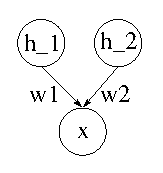
\includegraphics[width=0.45\columnwidth]{figures/explain_away1.eps}
    \end{minipage}
    \begin{minipage}{0.48\textwidth}
        \centering
        \psfrag{w1}[Tc][Tc][1][0]{$w_1$}
        \psfrag{w2}[Cc][Cc][1][0]{$w_2$}
        \psfrag{-5}[Tr][Tr][0.8][0]{$-5$}
        \psfrag{5}[Tr][Tr][0.8][0]{$5$}
        \psfrag{0}[Cl][Cl][1][0]{}
        \psfrag{0.2}[Cl][Cl][0.8][0]{$0.2$}
        \psfrag{-0.2}[Cl][Cl][0.8][0]{$-0.2$}
        \psfrag{-0.4}[Cl][Cl][0.8][0]{$-0.4$}
        \psfrag{-0.6}[Cl][Cl][0.8][0]{$-0.6$}
        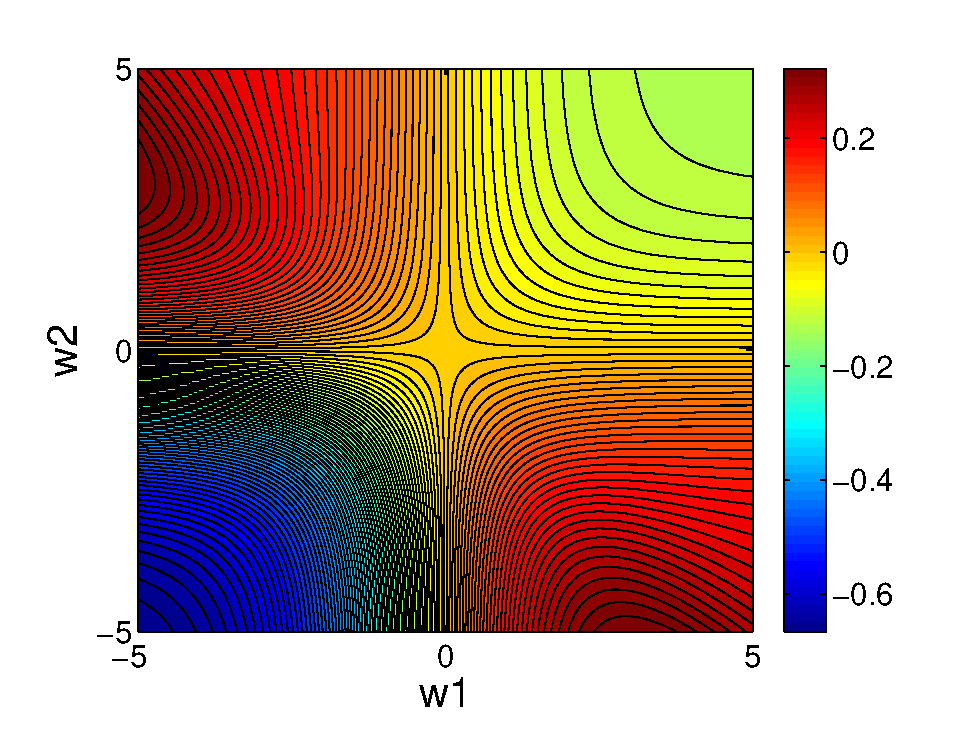
\includegraphics[width=0.85\columnwidth]{figures/explaining_away.eps}
    \end{minipage}
    \begin{minipage}{0.48\textwidth}
        \centering
        \small
        (a)
    \end{minipage}
    \begin{minipage}{0.48\textwidth}
        \centering
        \small
        (b) 
    \end{minipage}
    \caption{(a) A simple sigmoid belief network with two
    hidden units and a single visible unit. (b) The
    log-ratio
    between $p(h_2=1\mid x=1, h_1=1)$ and $p(h_2=1\mid
    x=1)$.}
    \label{fig:explaining_away}
\end{figure}

As an example, let us consider a sigmoid belief network
consisting of only two hidden units and a single visible
unit in Fig.~\ref{fig:explaining_away}(a). The two hidden
units $h_1$ and $h_2$ are a priori mutually independent
while each is equally likely to be either $0$ or $1$. The
conditional probability of the visible unit $x$ is defined
by 
\begin{align*}
    p(x = 1 \mid h_1, h_2) = \phi(w_1 h_1 + w_2 h_3),
\end{align*}
where $\phi$ is a logistic sigmoid function.

Under this model, the factorial assumption in the
approximate posterior states that 
\begin{align}
    \label{eq:cond_ind}
    p(h_2 = 1 \mid x = 1, h_1 = 1) = p(h_2 = 1 \mid x = 1,
    h_1 = 0),
\end{align}
since $h_2$ and $h_1$ are independent from each other
conditioned on $x$. 
%However, it is easy to see that
%Eq.~\eqref{eq:cond_ind} is highly unlikely to hold.

The conditional probability of $h_2$ being $1$ given $x=1$
and $h_1=1$ is 
\begin{align}
    \label{eq:compet_1}
    p(h_2 = 1 \mid x=1, h_1=1) = \frac{\phi(w_1 +
    w_2)}{\phi(w_1) + \phi(w_1 + w_2)},
\end{align}
and that given $x=1$ and $h_1=0$ is
\begin{align}
    \label{eq:compet_2}
    p(h_2 = 1 \mid x = 1, h_1 =0) = \frac{\phi(w_2)}{0.5 +
    \phi(w_1 + w_2)}.
\end{align}
These are unlikely to be identical, unless $w_1=0$, which
means that $h_1$ and $x$ are effectively disconnected. 

It is also interesting to see how the state of $h_1$ affects
the state of $h_2$. For instance, we can compare
Eq.~\eqref{eq:compet_1} against the conditional probability
of $h_2=1$ given $x=1$ after marginalizing out $h_1$.
Fig.~\ref{fig:explaining_away}(b) shows 
\begin{align*}
    \log\frac{p(h_2 = 1 \mid x=1, h_1 = 1)}{p(h_2=1 \mid
    x=1)},
\end{align*}
where
\begin{align*}
    p(h_2 = 1 \mid x = 1) = \frac{\phi(w_2) +
    \phi(w_1+w_2)}{\phi(0) + \phi(w_1) + \phi(w_2) +
    \phi(w_1+w_2)}.
\end{align*}

From this figure, we can see that the fact that $h_1$ is
known to have caused $x=1$ ($x=1,h_1=1$) decreases the
conditional probability of $h_2$ being the cause of $x=1$,
when both $w_1$ and $w_2$ are larger than zero. When the
signs of the weights are different, the opposite happens.

Intuitively speaking, if $h_1$, which is likely to have
triggered an observed event ($w_1 > 0$), has been found to
be true ($h_1=1$), it is unlikely that $h_2$, which is as
well likely to have triggered the event ($w_2 > 0$), has
happened also. Furthermore, if $h_1$ which is known to decrease
the likelihood of the observed event happening ($w_1 < 0$)
happened, $h_2$ which is known to increase the likelihood of
the event ($w_2 > 0$), is more likely to have triggered the
event.  This same phenomenon, called explaining away,
happens when we consider the posterior probability of $h_1$
when $h_2$ was observed to be $1$. 

The factorial approximation of posterior distribution of the
recognition process of sigmoid belief network, or of the
encoder of an autoencoder, however, is unable to incorporate
this competition between hidden units.

\subsubsection{Sparse Coding and Predictive Sparse
Decomposition}
\label{sec:sparse_coding}

Sparse coding \citep[see, e.g.,][]{Olshausen1996} is another
linear generative method which aims to learn a latent
variable model in Eq.~\eqref{eq:lvm}. There are two
important characteristics that distinguish sparse coding
from other methods such as PCA based on a linear generative
model.

Firstly, sparse coding typically assumes that there are more hidden
units ($q$) than visible units ($p$). It is usual to use $q = c \times
p$ with the constant $c \geq 2$. Secondly, it requires that
the number of nonzero components of $\vh$ be strictly below
a certain level $\rho$.

Given a set of training samples $D=\left\{ \vx^{(1)}, \dots
\vx^{(N)} \right\}$ sparse coding aims to find a set of
weights $\mW$ and a set of \textit{sparse code}s $\left\{
\vh^{(1)}, \dots, \vh^{(N)} \right\}$ by minimizing the
following cost function:
\begin{align}
    \label{eq:sp_cost_orig}
    \sum_{n=1}^N \left\| \vx^{(n)} - \mW \vh^{(n)}
    \right\|_2^2
\end{align}
subject to
\begin{align}
    \label{eq:sp_const_orig}
    \| \vh^{(n)} \|_0 \leq \tau\text{, }\forall n=1,\dots,N,
\end{align}
where $\tau=\rho q$ is a predefined level of sparsity. Similarly, we
may rewrite the cost function and the constraint as
\begin{align}
    \label{eq:cs_cost}
    \| \vh^{(n)} \|_0 \text{, }\forall n=1,\dots,N,
\end{align}
subject to
\begin{align*}
    \left\| \vx^{(n)} - \mW \vh^{(n)} \right\|_2^2 \leq
    \epsilon\text{, }\forall n=1,\dots,N,
\end{align*}
where $\epsilon$ is a bound on the reconstruction error.

Since it is often difficult to minimize the cost function in
Eq.~\eqref{eq:cs_cost} directly, it is usual to relax the
problem by minimizing the $L_2$ reconstruction error while
regularizing the $L_1$-norm of sparse codes, that is,
\begin{align}
    \label{eq:sp_cost}
    \argmin_{\mW, \left\{ \vh^{(n)} \right\}_{n=1}^N }
    \sum_{n=1}^N \left\| \vx^{(n)} - \mW \vh^{(n)}
    \right\|_2^2 + \lambda \sum_{n=1}^N \| \vh^{(n)} \|_1.
\end{align}

Unlike an autoencoder which has an explicit encoder that
outputs a hidden representation of a given input, in the
framework of sparse coding, the sparse code must be found
via optimization, for instance by an orthogonal matching
pursuit (OMP\nomenclature{OMP}{Orthogonal matching pursuit}) algorithm \citep{Davis1994}.

Most of those algorithms basically start from an all-zero
code and sequentially search for a hidden unit that
satisfies a certain criterion such as the reduction in the
reconstruction error. The search continues until the number
of non-zero components reaches the predefined level $L$.
This sequential process, in effect, avoids the problem of
the factorial assumption made by the encoder of an
autoencoder described earlier. 

For instance, let us consider the OMP. At each step of the
algorithm, let us assume that there are two hidden units
$h_1$ and $h_2$ that have the corresponding weight vectors
$\vw_1$ and $\vw_2$ whose inner products with a residual
vector $\vr$ are large, compared to other hidden units. From
a generative modeling perspective, $h_1$ and $h_2$ generate
a similar pattern in the visible units.

Assuming that $\left< \vw_1, \vr\right> = \left< \vw_2,
\vr\right> + \epsilon$ where $\epsilon$ is a very small
positive constant, the OMP will choose $h_1$ instead of $h_2$. Once
$\vw_1$ is included in the chosen bases, it is unlikely that
at any step later $h_2$, and correspondingly its basis
$\vw_2$, will be chosen as the $\vr$ afterward is almost
orthogonal to $\vw_2$. In essence, when $h_1$ was chosen, it
\textit{explained away} $h_2$.

Irrespective of this preferable property of sparse coding,
the computational cost of inferring the states of hidden
units is much higher compared to autoencoders. Hence, there
have been attempts to combine sparse coding together with a
parameterized encoder of an autoencoder to construct a model
that can implement, at least approximately, both
\textit{explaining away} and \textit{fast inference}
\citep[see, e.g.,][]{Kavukcuoglu2010,Gregor2010}.

In the case of \citep{Kavukcuoglu2010}, the regular sparse
coding cost function in Eq.~\eqref{eq:sp_cost} is augmented
with another regularization term that penalizes the
difference between the sparse code $\left\{ \vh^{(n)}
\right\}_{n=1}^N$ and the predicted sparse code computed by
a parameterized nonlinear encoder $f$. This model, called
predictive sparse decomposition
(PSD\nomenclature{PSD}{Predictive sparse decomposition}), solves the following
problem:
\begin{align*}
    \argmin_{\mW, \left\{ \vh^{(n)}, \TT_f \right\}_{n=1}^N }
    &\sum_{n=1}^N \left\| \vx^{(n)} - \mW \vh^{(n)}
    \right\|_2^2 + \\
    &\phantom{\sum_{n=1}^N }\lambda \sum_{n=1}^N \| \vh^{(n)} \|_1 
    + 
    \alpha \sum_{n=1}^N \| \vh^{(n)} - f(\vx^{(n)} \mid
    \TT_f) \|_2^2,
\end{align*}
where $\TT_f$ is a set of parameters that define the encoder
$f$, and $\alpha$ is a constant that balances between the
encoder $f$ and the optimal hidden states.

The underlying principle of the PSD is similar to that of
the GP-LVM with a back-constraint described earlier.  In an
original formulation of sparse coding, decoding is
straightforward and computationally cheaper, while encoding
is not. Hence, the computationally expensive encoding step
is approximated by a nonlinear parametric, potentially
multi-layered encoder.

\subsubsection{Sparse Autoencoder and Explicit Sparsification}
\label{sec:spaenc}

Let us consider an autoencoder with only a single
intermediate layer of sigmoid hidden units. In this case, we
have already discussed that its encoder can be considered as
performing an approximate inference of the factorial
posterior distribution of the hidden units given a state of
the visible units. In the approximate factorial posterior
distribution, each hidden unit follows a Bernoulli
distribution with its mean computed by the encoder such that
\begin{align*}
    p(h_j = 1 \mid \vx, \TT) = \phi\left( \sum_{i=1}^p
    w_{ij} x_i + c_j \right),
\end{align*}
for all $j=1,\dots,q$.

Under this interpretation, it is possible for us to
regularize the autoencoder such that on average over
training samples, each hidden unit is unlikely to be active.
Equivalently, the probability of each hidden unit being
active should on average be low.

The autoencoder regularized to have a low average hidden
activation probability is called a \textit{sparse}
autoencoder. One of the most widely used regularization term
was proposed by \citet{Lee2007}:
\begin{align}
    \label{eq:srbm_reg}
    \Omega(\TT, D) = \frac{1}{q} \sum_{j=1}^q \frac{1}{2} \left|
    \frac{1}{N} \sum_{n=1}^N \hat{h}_j^{(n)} - \rho
    \right|^2,
\end{align}
where $\rho$ is a target hidden activation probability and
\[
\hat{h}_j^{(n)} = p(h_j = 1 \mid \vx^{(n)}, \TT).
\]
Instead of the squared Euclidean distance, one may use the
Kullback-Leibler (KL) distance such that
\begin{align*}
    \Omega(\TT, D) = \frac{1}{N} \sum_{n=1}^N 
    \frac{1}{q} \sum_{j=1}^q \left( \rho \log
    \frac{\rho}{\hat{h}_j^{(n)}} + (1 - \rho) \log \frac{1 -
    \rho}{1 - \hat{h}_j^{(n)}} \right).
\end{align*}

There are other possibilities to learn a sparse autoencoder,
for instance, by a sparse encoding symmetric machine
(SESM\nomenclature{SESM}{Sparse encoding symmetric machine})
proposed by \citet{Ranzato2008}. However, here, we stick to
the regularization based on Eq.~\eqref{eq:srbm_reg}.

If we consider any model that has hidden units, we find that
either encoding (autoencoders) or inference (probabilistic
PCA and sparse coding) is equivalent to a (nonlinear)
mapping $f$ that has its domain $\PP \subseteq \RR^p$
and range $\QQ \subseteq \RR^q$. $\PP$ is naturally defined
by the set of training samples, while $\QQ$ is defined by a
regularization term. For instance, the range of the encoder
of a regular PCA, which does not have any regularization or
constraint, is unrestricted and equals to $\RR^q$.

However the inference procedure of sparse
coding, for instance, according to the constraint in
Eq.~\eqref{eq:sp_const_orig}, maps an input $\vx \in \PP$ to
$\QQ$ which includes only those points $\vh$ that satisfy 
\[
\| \vh \|_0 \leq \tau,
\]
for some constant $\tau > 0$. Similarly, the encoder of a
sparse autoencoder trained with the sparsity regularization
in Eq.~\eqref{eq:srbm_reg} has the (approximate) range $\QQ
\subseteq \RR^q$ such that 
\begin{align}
    \label{eq:f_range}
    \QQ \approx \left\{\vh = f(\vx) \left| \vx \in \PP, \left\|
    \E_{\vx \in \PP}\left[ h_j \right] - \rho \right\|_2^2 =
    0 \right.\right\}
\end{align}
with the amount of error controlled by the regularization
constant.

In the case of a sparse autoencoder, mapping $f(\vx)$ of any
sample $\vx$ that is close to one of the training samples will
fall in $\QQ$. In other words, the average activation of
$f(\vx)$ will be around the predefined $\rho$. If the
average activation of $f(\vx)$ is either much smaller or
much larger than $\rho$, it can be suspected that the sample
$\vx$ is either not the same type as training samples or
corrupted with high level of noise.

This leads to the idea of explicit sparsification, proposed
in \citepub{Cho2013icml}. It is claimed that the encoded
state of hidden units of a sparse autoencoder should not be
used as it is. Rather, it must be checked whether $\vh =
f(\tilde{\vx})$ belongs to $\QQ$, and if not, $\vh$ needs to
be projected on or nearby $\QQ$ by an explicit
sparsification.

An explicit sparsification $R$ is defined by 
\begin{align}
    \label{eq:esp}
    R(\vh) = \argmin_{\vq \in \QQ} d(\vh - \vq),
\end{align}
where $d(\cdot, \cdot)$ is a suitable distance metric.

One simple way to explicitly sparsify $f(\vx)$ is to use a
\textit{simple sparsification} which effectively sets small
components to zero by
\begin{align}
    \label{eq:simple_sparsification}
    \vh \leftarrow \max\left(\vh - \max\left(\frac{1}{q}
    \|\vh\|_1 - \left(1 - \bar{\rho}\right), 0\right),
    0\right),
\end{align}
where $\max$ applies to each component. It is obvious to see
that $\bar{\rho}$ which defines a target sparsity, should be
set to one minus the target hidden activation probability
$\rho$ in Eq.~\eqref{eq:srbm_reg}.

This simple approach was empirically shown to be effective
when a sparse autoencoder trained on clean samples was
applied to novel samples which were corrupted with high
level of noise in \citepub{Cho2013icml}. The two tasks
considered in \citepub{Cho2013icml} were image
denoising and classifying highly corrupted test
samples. In both cases, more robust performance could be
achieved if the activations of the units in the bottleneck
were treated with the proposed simple sparsification.

\section{Manifold Assumption and Regularized Autoencoders}
\label{sec:dae_cae}

The manifold\footnote{ For more details on manifolds, we refer any
interested reader to \citep{Absil2008}.}assumption \citep{Chapelle2006} states
that
\textit{
the (high-dimensional) data lie (roughly) on a
low-dimensional manifold.
}

Informally, it says that a (small) neighborhood or chart
$U_\vx$ surrounding each data sample $\vx \in \RR^p$ which
lies on a manifold $\MM \subset \RR^p$ has a bijection
$\varphi$ onto an open subset of a $d$-dimensional Euclidean
space $\RR^d$, where $d \ll p$.
Any other point $\vx'$ in the neighborhood $U_\vx$ can be
reached from $\vx$ by 
\[
\vx' = \varphi^{-1} \left( \varphi(\vx) + \epsilon \right),
\]
where $\epsilon \in \RR^d$. Thus, the degree of freedom is
$d$ which is smaller than $p$.

Intuitively, this says that the number of local variations
in the above case $q$, allowed for a sample to remain 
on the manifold, is smaller than the dimensionality $p$ of
the original space to which it belongs to. Furthermore, any
other variation pushes the sample outside the manifold,
making it invalid, or a noisy sample of the data.

Under this assumption, it is desirable to transform the
coordinate system of an original space into one that
describes the variations allowed on the manifold only. In
other words, we want the transformation to \textit{capture}
and \textit{disentangle} the hidden, underlying factors of
variations \citep{Bengio2009a} while ignoring any possible
variation in the original space that moves away from the
manifold. These transformed coordinates hopefully will
improve the performance of a target task using another
model. For instance, \citet{Bengio2013} recently
conjectured and provided empirical evidence that this
disentangling, or transformation, results in better mixing
of MCMC chains as well as an improvement in classification
tasks.

One prominent example that implements this
manifold assumption is principal component analysis
(PCA), discussed earlier in
Section~\ref{sec:linear_autoencoder}. PCA assumes that
the manifold on which training samples lie is
\textit{linear}. The linear manifold is described by the few
largest principal components which correspond to the
directions of maximal variance \citep[see,
e.g.,][]{Bishop2006}. Any change along the directions of small variances, or
few last principal components, is mainly considered as
%to correspond to 
meaningless
noise. However, the linear nature of PCA is highly
restrictive, in the sense that in many problems most interesting factors of
variations are unlikely to be linear, which is one of the
reasons that motivated introducing deep neural networks with
nonlinear hidden units.

In fact, an MLP with multiple intermediate hidden layers can
be seen as capturing the data manifold and performing
classification on the captured manifold. As discussed
earlier in Section~\ref{sec:mlp}, each pair of two
consecutive non-output layers nonlinearly transforms the
coordinates of the input from the lower layer. If each of
them can gradually capture and disentangle the factors of
variations along the manifold on which training samples lie,
we can expect that the top two layers which perform the
actual target task, either classification or regression,
will benefit from it.

Unless we are lucky, however, we cannot expect that this type of
transformation that captures the data manifold will be
discovered when
we estimate the parameters of an MLP. It might happen that
minimizing the cost function in Eq.~\eqref{eq:mlp_cost} ends
up in the (local) solution that corresponds to the situation
where intermediate hidden layers gradually capture the data
manifold, but it is not likely nor guaranteed.

Instead, there is another approach that gradually builds up
a sequence of transformations, starting from the raw data.
This incremental way of transforming coordinates is known
widely as a greedy layer-wise pretraining
\citep{Hinton2006}. This will be discussed more in
Chapter~\ref{chap:pretraining}, and in the remainder of this
section we will look at two variants of autoencoders that
are known to capture the data manifold. These two models
have been recently shown to be good candidates for gradually
capturing the data manifold.


\subsection{Denoising Autoencoder and Explicit Noise
Injection}
\label{sec:dae}

%Similarly, when an autoencoder is trained with
%stochastically corrupted training samples, the
%reconstruction of the resulting autoencoder is insensitive
%to the small amount of noise in an input and able to
%\textit{denoise} a noisy sample
%\citep{Jain2008,Vincent2010}. 

Instead of our original aim of training an autoencoder, we
may decide to train it to \textit{denoise} a noisy sample so
that 
\[
\vx \approx g(f(\tilde{\vx})),
\]
where $\vx$ and $\tilde{\vx}$ are clean and noisy versions
of the same sample, and $f$ and $g$ are the encoder and
decoder of the autoencoder, respectively. 

Naturally, this can be done trivially by modifying the cost
function in Eq.~\eqref{eq:autoencoder_cost} so that noise is
explicitly injected before the encoder is applied to
training samples.  When the cost function is modified
accordingly, we call the resulting autoencoder a
\textit{denoising} autoencoder \citep{Vincent2010}. 

A denoising autoencoder is constructed to have in many
cases a single intermediate hidden layer. The parameters
are estimated by minimizing the following cost function:
\begin{align}
    \label{eq:dae_cost}
    J(\TT) =  \sum_{n=1}^N \left\| \vx^{(n)} -
    g\left(f(\kappa(\vx^{(n)}))\right)
    \right\|_2^2,
\end{align}
where $f$ and $g$ are respectively the encoder and decoder
defined by Eqs.~\eqref{eq:ae_encoder} and
\eqref{eq:ae_decoder}.  $\kappa$ is a stochastic operator
that adds 
%zero-mean 
random noise to the input\footnote{
$\kappa(\vx)$ may be designed to corrupt the input using the
combination of multiple types of noise. In
\citep{Vincent2010}, the following types of noise were
proposed:
\begin{enumerate}
        \vspace{-5mm}
    \itemsep 0em
    \item Additive white Gaussian: add white Gaussian noise
        to each component
    \item Masking: randomly force some components to $0$
    \item Salt-and-Pepper noise: randomly force some
        components to either the maximum or minimum allowed
        value
\end{enumerate}
}.

The denoising autoencoder finds a coordinate system of the
data manifold.
%without any assumption, for
%instance, of the linearity. 
Minimizing Eq.~\eqref{eq:dae_cost} effectively corresponds
to \textit{ignoring} any direction of variation injected by
$\kappa$. This is equivalent to maintaining only those
directions that are implicitly found by the training samples
\citep{Vincent2010}. From this, we may say that the
denoising autoencoder learns the data manifold, since the
data manifold is by definition a set of small
neighborhoods (charts) that encode those directions of
variations.

Here let us in more detail try to understand at least
informally how the denoising autoencoder internally
\textit{learns} the data manifold. We will consider a
denoising autoencoder with a single intermediate hidden
layer only.

Let $\vx$ and $\vx'$ be two nearby real-valued training
samples, and $\vh=f(\vx)$ and $\vh'=f(\vx')$ are
corresponding hidden states encoded by a denoising
autoencoder. We assume that $\kappa$ was chosen to add a
white Gaussian noise.

If we consider only $\vx$, because we trained the denoising
autoencoder by minimizing Eq.~\eqref{eq:dae_cost}, any point
$\vx + \epsilon$ in a small area surrounding $\vx$, defined
by $\kappa$, will map almost exactly to $\vh$. This applies
to $\vx'$ as well. 

However, we should pay attention to a point $\bar{\vx}$ in
an \textit{overlapping} area. For instance, a middle point
$\bar{\vx} = \frac{\vx + \vx'}{2}$ between $\vx$ and $\vx'$
will neither be reconstructed exactly to $\vx$ nor $\vx'$.
Instead, it will be reconstructed to be a point between
$\vx$ and $\vx'$, and because the decoder is linear, the
hidden state of $\bar{\vx}$ will also lie between $\vh$ and
$\vh'$. See Fig.~\ref{fig:dae_manifold} for illustration.

\begin{figure}[t]
    \centering
    \psfrag{hidden}[Bc][Bc][1][0]{Hidden space}
    \psfrag{data}[Bl][Bl][1][0]{Data space}
    \psfrag{k(x)}[Bc][Tc][1][0]{$\kappa(\vx)$}
    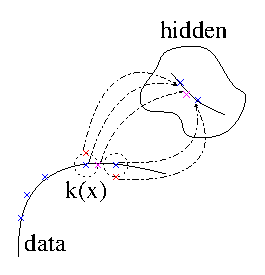
\includegraphics[width=0.75\columnwidth]{figures/dae.eps}
    \caption{Illustration of how a denoising autoencoder
    learns a data manifold. The solid curves are the
    manifolds on which the training samples in the data
    space and their corresponding representations in the
    hidden space lie.  The blue points
    (\textcolor{blue}{$\times$}) correspond to both training
    samples in the data space and their hidden
    representations in the hidden space ($\vx$, $\vx'$ and
    $f(\vx)$, $f(\vx')$ in the text). The dashed circle
    around a training sample shows the amount of error
    explicitly injected by $\kappa$. The red points
    (\textcolor{red}{$\times$}) are examples of the
    neighboring points of the training samples that are
    \textit{not} on the data manifold, while the magenta
    point (\textcolor{magenta}{$\times$}) lies on the
    manifold between two training samples ($\bar{\vx}$ and
    $f(\bar{\vx})$ in
    the text). The deviations of
    both the red points from their original training samples
    are ignored in the encoder, while that of the magenta
    point is preserved.}
    \label{fig:dae_manifold}
\end{figure}

In short, the change in a hidden representation encoded by
the denoising autoencoder corresponds \textit{only} to the
change on the manifold on which training samples lie. Any
other small change in directions moving outside the manifold
will be ignored. In this way, a denoising autoencoder learns
the data manifold.

This, however, does not mean that every possible state of
the hidden units encodes a point on the data manifold. It is
not well defined nor known to what extent points far from the
manifold will be encoded. Fortunately, this may not be a big
problem when we deal with a task where both training and
test samples were obtained from a single
distribution whose probability mass is mostly concentrated
along the manifold. This will eliminate any need of encoding
a sample far away from the manifold.

As can be expected from this argument, it has been shown by,
for instance, \citet{Vincent2010}
%, and later by other
%researchers \citep[see, e.g.,][and references therein]{Bengio2009a}, 
that the
denoising autoencoder tends to learn a \textit{better}
representation that is more suitable for a further machine
learning task such as classification than the one extracted
by an ordinary autoencoder. Therefore, this model
has been used widely to pretrain an MLP layer-wise.

\subsubsection{Explicit Noise Injection for Classification}
\label{sec:noise_injection}

Let us now discuss briefly another aspect of injecting random
noise explicitly to training samples while estimating
parameters.

It is usual that we know \textit{a priori} that the data
distribution from which the training samples as well as
the test samples are sampled is smooth with respect to each
point in the state space. In supervised learning, this
means that a point $\vx$ which is not necessarily in a
training set but in the neighborhood of a training sample
$\vx^{(n)}$, is highly likely to belong to the same class
$y^{(n)}$. In unsupervised learning, it means that a point
$\vx$, again in the neighborhood of a training sample
$\vx^{(n)}$, is likely to have a similar probability.

If we go one step further, we may say that there is a
certain invariance with respect to some transformation,
potentially nonlinear and stochastic, $\kappa$ such that
$\kappa(\vx)$ is similar, or has a similar property to
$\vx$. The property shared by those two points may be their
classes or their probabilities in the data distribution.

An extremely easy and obvious way to incorporate this prior
knowledge is to use corrupted or transformed versions of
training samples $\left\{ \vx^{(n)} \right\}_{n=1}^N$ when
estimating the parameters of a model \citep[see,
e.g.,][Chapter 5.5]{Bishop2006}. 

For instance, in the case of an MLP, the aim of the neural
network is to find a nonlinear mapping from an input to its
corresponding output. The above prior knowledge, however,
suggests that rather than trying to optimize the network to
find the mapping from the raw training set, the network
needs to be optimized to find the mapping from a transformed
input $\kappa(\vx^{(n)})$ to its output $y^{(n)}$. Then, the
cost function originally in the form of
Eq.~\eqref{eq:mlp_cost}, is replaced by
\begin{align}
    \label{eq:mlp_cost_noisy}
    J(\TT) = \sum_{n=1}^N d\left(y^{(n)},
    u(\kappa(\vx^{(n)}))\right),
\end{align}
where $u(\cdot)$ is the output of the MLP.

If we assume that $\kappa$ stochastically corrupts the
input,
%\footnote{From here on, we will say that $\kappa$
%\textit{corrupts} the input, as our main focus in this
%section is to build a model that is robust to \textit{noise}
%only.  }
thus making a noisy version of it, the trained MLP becomes
more \textit{robust} to noise in the input. In other words,
the input corrupted by some level of noise will nevertheless
be mapped to its desired output which is the output expected
from the clean input. 

It is natural to use the stochastic gradient method
described in Section~\ref{sec:stochastic_grad} to minimize
Eq.~\eqref{eq:mlp_cost_noisy}. At each iteration, a randomly
chosen subset of the training set is stochastically
corrupted by $\kappa$ before the steepest descent direction
is computed. 

In the case where $\kappa$ simply adds uncorrelated white
Gaussian noise to an input, \citet{Bishop1995} showed that
minimizing Eq.~\eqref{eq:mlp_cost_noisy} is related to
regularizing the sensitivity of an output with respect to
the input such that the cost function to be minimized
becomes
\begin{align}
    \label{eq:noise_injection_reg}
    J(\TT) = \sum_{n=1}^N d\left(y^{(n)},
    u(\vx^{(n)})\right) + \frac{\lambda}{2}
    \sum_{i=1}^p \sum_{j=1}^q \left( \frac{\partial
    u(\vx^{(n)})}{\partial \vx^{(n)}}\right)^2,
\end{align}
where the regularization constant $\lambda$ is determined by
the amount of noise injected by $\kappa$ in
Eq.~\eqref{eq:mlp_cost_noisy}.

\subsection{Contractive Autoencoder}

The informal discussion in Section~\ref{sec:dae} on how the
denoising autoencoder learns the data manifold, arrives at
the conclusion that the key is the invariance of
hidden activations to any direction of change moving outside
the manifold. Or, it may be said that any infinitesimal
change to a point in the data space should not change its
corresponding encoded point in the hidden space.  In other
words, the norm of the Jacobian matrix $J_f$ should be
minimized. The Jacobian matrix $J_f \in \RR^{q \times p}$
with respect to the encoder $f$ is defined as
\begin{align}
    \label{eq:jacob_f}
    J_f = \left[ 
    \begin{array}{c c c}
        \frac{\partial \hat{h}_1}{\partial x_1} & \cdots &
        \frac{\partial \hat{h}_1}{\partial x_p} \\
        \vdots & \ddots & \vdots \\
        \frac{\partial \hat{h}_q}{\partial x_1} & \cdots & \frac{\partial \hat{h}_q}{\partial x_p}
    \end{array}
    \right],
\end{align}
where $\hat{h}_j$ is the $j$-th component of $f(\vx)$.

A denoising autoencoder achieves this by injecting
predefined levels of noise to training samples. However,
this does not directly minimize $J_f$, as we have seen
previously in Eq.~\eqref{eq:noise_injection_reg}, it rather
penalizes $J_{g \circ f}$ which is 
\begin{align*}
    J_{g \circ f} = \left[ 
    \begin{array}{c c c}
        \frac{\partial \tilde{x}_1}{\partial x_1} & \cdots &
        \frac{\partial \tilde{x}_1}{\partial x_p} \\
        \vdots & \ddots & \vdots \\
        \frac{\partial \tilde{x}_q}{\partial x_1} & \cdots &
        \frac{\partial \tilde{x}_q}{\partial x_p}
    \end{array}
    \right],
\end{align*}
where $\tilde{x}_j$ is the $j$-th component of the
reconstruction.

Hence, \citet{Rifai2011} proposed to directly regularize the
$L_2$-norm of $J_f$ by adding the following regularization
term to the cost function based on reconstruction error
\begin{align}
    \label{eq:cae}
    \Omega(D, \TT) = \sum_{\vx \in D} \sum_{i=1}^p \sum_{j=1}^q
    \left( \frac{\partial \hat{h}_j}{\partial x_i}
    \right)^2.
\end{align}
Furthermore, \citet{Rifai2011ho} proposed to
regularize, in addition to the Jacobian, the Hessian $H_f$
approximated using the finite-difference method by modifying
Eq.~\eqref{eq:cae} to
\begin{align*}
    \Omega(D, \TT) = \sum_{\vx \in D} \sum_{i=1}^p \sum_{j=1}^q
    \left( \frac{\partial \hat{h}_j}{\partial x_i}
    \right)^2 + \gamma \sum_{i=1}^p \sum_{j=1}^q \E_{\epsilon} \left[ 
    \left( \frac{\partial \hat{h}_j}{\partial x_i}(x_i)
    - \frac{\partial \hat{h}_j}{\partial x_i}(x_i +
    \epsilon)
    \right)^2
    \right],
\end{align*}
where $\epsilon \sim \N(0, \sigma^2)$.

This idea of utilizing the Jacobian matrix with respect to
each training sample suggests to further use the Jacobian
matrix to investigate the local neighborhood, or chart,
centered on the training sample. The leading singular
vectors or principal components of the Jacobian matrix are
the directions parallel to the data manifold, while the
minor singular vectors indicate those directions that are
close to perpendicular to the manifold.

If the manifold assumption at the beginning of this section
indeed holds true and the contractive regularization in
Eq.~\eqref{eq:cae} enables the autoencoder to capture this
manifold, only few leading singular vectors will have a large
corresponding singular value, while the others will be
close to zero. In other words, the neighborhood
centered on each training sample will have only a few
degrees of freedom which correspond to the leading singular
vectors.

\citet{Rifai2011} empirically showed that this is indeed the
case with the autoencoders trained with the contractive
regularization (Eq.~\eqref{eq:cae}) as well as the denoising
autoencoders. The phenomenon was most visible when the
contractive regularization was used, which suggests that
directly regularizing the Jacobian matrix may help capturing
the data manifold more effectively and efficiently.

A similar idea was applied to training restricted Boltzmann
machines (see Section~\ref{sec:rbm}) in
\citepub{Cho2012icann}.
%, however, without much success.


\section{Backpropagation for Feedforward Neural Networks}
\label{sec:backprop}

Before finishing our discussion on deep feedforward neural
networks, in this section, we briefly describe an efficient
algorithm that computes the gradient of a cost function with
respect to each parameter of a deep feedforward neural
network. The algorithm, called backpropagation\footnote{
The name \textit{backpropagation} was coined by
\citet{Rumelhart1986} to denote a learning algorithm for
estimating the parameters of a multi-layer perceptron.
However, the main idea underlying backpropagation is to use
a chain rule to compute the gradient of a cost function with
respect to the parameters of a multi-layer perceptron, and
the computed gradient may be used with any learning
algorithm that utilizes it. It has, hence, become more
common to use the term backpropagation to refer to the
algorithm that computes the gradient, separate from an
algorithm that adjusts the parameters using the computed
gradient.  However, in this thesis, we refer by
\textit{backpropagation} a learning algorithm that adjusts
the parameters of a multi-layer perceptron using the
gradient computed using the chain rule.
}, was proposed
by \citet{Rumelhart1986}.

In order to compute the gradient, we first perform a
\textit{forward} pass. For each sample $\vx$, we recursively
compute the activation of the $j$-th hidden unit
$h_j^{\qlay{l}}$
at the $l$-th hidden layer by
\[
h_j^{\qlay{l}} = \phi_j^{\qlay{l}}
\left(\sum_{k=1}^{q_{\qlay{l-1}}} h_k^{\qlay{l-1}}
w_{kj}^{\qlay{l}}\right),
\]
where the activation of the $j$-th hidden unit in the first
hidden layer is
\[
h_j^{\qlay{1}} = \phi_j^{\qlay{1}} \left(\sum_{i=1}^p x_i
w_{ij}^{\qlay{1}}\right)
\]
and the activation of the $j$-th linear output unit is 
\[
u_j(\vx) = \phi_j^{o} \left( \sum_{k=1}^{q_{\qlay{L}}}
h_{k}^{\qlay{L}} u_{kj}
\right).
\]
Note that we used a different notation for the nonlinear
function of each unit, other than visible ones, to emphasize
that the algorithm works in a general feedforward neural
network. 
%To make equations uncluttered, 
For simplicity, we have omitted biases without loss of
generality.

After the forward pass, we begin the \textit{backward} pass,
where a local gradient $\delta$ is computed per each unit.
For each output unit, where a desired output $y_j$ is
available, the local gradient is
\[
\delta_j = \frac{\partial J}{\partial u_j} 
\]
which is simply a difference between the predicted and
desired values:
\[
\delta_j = y_j - u_j(\vx),
\]
assuming that the output units are linear
($\phi_j^o(x) = x$) and the cost function $J$ is defined
based on the squared Euclidean distance between the true and
predicted outputs. The same computation holds when the
cross-entropy loss is used together with the sigmoid output
units.

For a hidden unit in a subsequent intermediate layers, we
compute the local gradients recursively using the backward
pass
%, hence, a backward pass, 
by
\[
\delta_j^{\qlay{l-1}} = \left(h_j^{\qlay{l-1}}\right)'
\sum_{k=1}^{q_{\qlay{l}}}
w_{jk}^{\qlay{l}} \delta_j^{\qlay{l}}
\]
until $l$ reaches $2$, where $\left(h_j^{\qlay{l-1}}\right)'$ is
the partial derivative of $h_j^{\qlay{l-1}}$ with respect to the
input to the unit. For instance, if the nonlinear function
used by the unit $\phi_j^{\qlay{l-1}}$ is a logistic sigmoid
function, then
\[
\left(h_j^{\qlay{l-1}}\right)' = h_j^{\qlay{l-1}} \left( 1 -
h_j^{\qlay{l-1}} \right).
\]

Once all the inputs and local gradients are computed, the
top-level and intermediate-level weight parameters $u_{kj}$
and $w_{ij}^{\qlay{l}}$ are respectively updated by
\begin{align}
    \label{eq:backprop}
    u_{kj} &\leftarrow u_{kj} - \eta \left( \delta_j
    h_k^{\qlay{L}}
    \right) 
    \nonumber \\
    w_{ij}^{\qlay{l}} &\leftarrow w_{ij}^{\qlay{l}} - \eta \left(
    \delta_j^{\qlay{l+1}} h_i^{\qlay{l-1}}\right) \text{, }\forall l \geq 2 
    \nonumber \\
    w_{ij}^{\qlay{1}} &\leftarrow w_{ij}^{\qlay{1}} - \eta \left(
    \delta_j^{\qlay{2}} x_i
    \right),
\end{align}
where $\eta$ is a learning rate. See Fig.~\ref{fig:backprop}
for the illustration of the forward and backward passes.

\begin{figure}[t]
    \centering
    \psfrag{x_1}[Bc][Bc][1][0]{$x_1$}
    \psfrag{x_2}[Bc][Bc][1][0]{$x_2$}
    \psfrag{x_p}[Bc][Bc][1][0]{$x_p$}
    \psfrag{h_1}[Bc][Bc][1][0]{$h^{(1)}_1$}
    \psfrag{h_2}[Bc][Bc][1][0]{$h^{(1)}_2$}
    \psfrag{h_q}[Bc][Bc][1][0]{$h^{(1)}_{q_1}$}
    \psfrag{z_1}[Bc][Bc][1][0]{$h^{(L)}_1$}
    \psfrag{z_2}[Bc][Bc][1][0]{$h^{(L)}_2$}
    \psfrag{z_q}[Bc][Bc][1][0]{$h^{(L)}_{q_L}$}
    \psfrag{t_n}[Bc][Bc][1][0]{$y$}
    \psfrag{y_n}[Bc][Bc][1][0]{$\hat{y}$}
    \psfrag{d_n}[Bc][Bc][1][0]{$\delta$}
    \psfrag{p_1}[Bc][Bc][1][0]{$\delta^{(L)}_1$}
    \psfrag{p_2}[Bc][Bc][1][0]{$\delta^{(L)}_2$}
    \psfrag{p_q}[Bc][Bc][1][0]{$\delta^{(L)}_{q_L}$}
    \psfrag{q_1}[Bc][Bc][1][0]{$\delta^{(1)}_1$}
    \psfrag{q_2}[Bc][Bc][1][0]{$\delta^{(1)}_2$}
    \psfrag{q_q}[Bc][Bc][1][0]{$\delta^{(1)}_{q_1}$}
    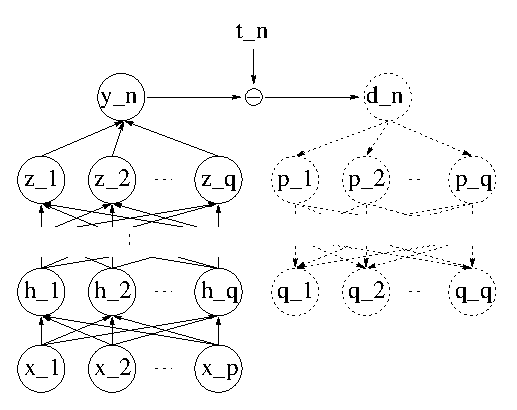
\includegraphics[width=0.75\columnwidth]{figures/mlp_bp.eps}
    \caption{An illustration of the forward and
    backward passes. Starting from the input layer on left,
    the activation of each unit is iteratively computed up
    until the output $\hat{y}$ is predicted. The difference
    $\delta$ between the prediction $\hat{y}$ and true
    output $y$ is computed, and the local gradients
    $\delta_j^{(l)}$ are iteratively computed in the
    backward pass. The left and right parts of the figure
    respectively correspond to the forward and backward
    passes.}
    \label{fig:backprop}
\end{figure}

The gradient of each weight parameter relies only on the
input and local gradient of the adjacent vertices. This
implies that the backpropagation is \textit{not} limited to
training a feedforward neural network, but may also be
applied to a recurrent neural network with a slight
modification (see Section~\ref{sec:rnn_deep} to see how a
recurrent neural network can be \textit{unfolded} over time
to become a deep feedforward neural network). 

Here we showed how to compute the gradient using a single
sample, but extending it to multiple samples is
straightforward by taking an average of
gradients computed from a number of samples at each update. It is usual to
use the gradient computed by the backpropagation to perform
stochastic gradient descent on the cost function using a
subset of training samples at a time (see
Section~\ref{sec:stochastic_grad}). One often refers to this
approach as \textit{stochastic backpropagation}.

\subsection{How to Make Lower Layers Useful}
\label{sec:bp_imp}

However, it has been noticed by many researchers that it is not easy to
train deep neural networks using plain stochastic
backpropagation \citep[see, e.g.,][]{Bengio2007a}.
Especially, neural networks with more than two intermediate
layers of hidden units usually result in a worse
generalization performance\footnote{By
\textit{generalization performance}, we refer to the
performance of a trained model on an unseen, novel sample.
} than those with only one or two intermediate layers
\citep{Bengio2007nips}.

One important hypothesis explaining the underlying
reasons for this phenomenon was proposed by
\citet{Bengio2007nips}. According to this hypothesis, this
difficulty may come from the fact that the parameters of the
lower layers (closer to a layer with input units) are poorly
estimated since \textit{the top three layers, consisting of
the output layer and two last hidden layers, are capable
enough of learning a given training set almost perfectly}.
They essentially act as a deep neural network with a single
intermediate hidden layer, which already has a universal
approximator property, using the activation of the hidden
units in the layer immediately below as an input. However,
this capability of the top two layers does not translate to
the performance of the neural network on unseen samples.

In other words, training an MLP with backpropagation will
simply adapt the parameters of the top layers to fit the
training set as well as possible. The algorithm in general
will \textit{not} necessarily prefer a solution that aims to
force the lower intermediate layers, which act as
\textit{feature detectors} according to our discussion in
Section~\ref{sec:mlp}, to detect important features.  A
simple experiment by \citet{Bengio2007nips} showed further
that even when the top layers are \textit{not} powerful
enough to minimize the cost function almost perfectly, the
plain stochastic backpropagation will fail to make the lower
intermediate layers any more useful.

In an extreme case, it might be that the top two layers, the
output and the last hidden layers, will be enough to minimize
the cost function almost perfectly. In this case, it is
possible that the network effectively becomes an extreme
learning machine, discussed in Section~\ref{sec:elm}, since
the weights of lower layers do not change from their
randomly initialized values. 

In order to avoid this problem, an approach that
incrementally adds intermediate layers starting from the
visible layer has been suggested by, for instance,
\citet{Fahlman1990} and \citet{Lengelle1996}.  The cascade
correlation algorithm \citep{Fahlman1990} starts from a
logistic regression network without any intermediate hidden
layer, and then incrementally trains and adds intermediate
layers while keeping all the existing connections as long as
the cost function decreases by doing so.
\citet{Lengelle1996} similarly add new intermediate layers,
or units, until the objective function based on the class
separability does not improve.  However, these approaches
based on supervised criteria have not been widely adopted as
they did not show much improvement.

\citet{Hinton2006} proposed a method called greedy
layer-wise pretraining which pretrains each pair of two
consecutive layers starting from the bottom two layers, as
if it were an restricted Boltzmann machine (see
Section~\ref{sec:rbm}). Similarly to the earlier attempts,
this approach allows stacking multiple layers. However, each
pair is trained in an \textit{unsupervised} manner, where
no output information is used during the layer-wise
pretraining. The success of this approach started a so
called \textit{second neural network renaissance}
\citep{Schmidhuber2011}.  We will discuss in more detail this
approach in Chapter~\ref{chap:pretraining}.

However, the hypothesis by \citet{Bengio2007nips} is not the
only explanation available.  \citet{Martens2010} pointed
out that another potential factor that makes it difficult to
estimate the parameters of lower layers of a deep MLP, or a
deep autoencoder by a plain backpropagation is the existence
of a pathological curvature of the cost function, not the
powerfulness of the top few layers. 

\citet{Martens2010} claimed that the directions of the cost
function that correspond to the parameters in the lower
layers have lower curvature compared to those corresponding
to the parameters in the top few layers. In this scenario,
the plain backpropagation, relying solely on the first-order
information, is unable to make rapid, if any, progress in
those directions with low curvatures, leaving the parameters
of the lower layers mostly unchanged.

The Hessian-free optimization, or truncated Newton method with
subsampled Hessian algorithms, proposed by
\citet{Martens2010} and \citet{Byrd2011} independently,
overcomes this problem by utilizing the Hessian of the cost
function. Specifically in the cases of deep autoencoders and
recurrent neural networks, \citet{Martens2010} and
\citet{Sutskever2011} empirically showed that the
Hessian-free optimization can indeed train very deep neural
networks without much difficulty. For a detailed discussion
on implementing the Hessian-free optimization for training
deep neural networks, we refer any interested reader to
\citep{Martens2012}.

In a similar sense, \citet{Raiko2012} proposed, instead of a
novel optimization algorithm, to linearly transform each
unit in a deep neural network such that the mean and the
first-derivative of the output of each unit are close to
zero. In order to make the neural network invariant under
such a transformation, shortcut connections skipping one or
few intermediate layers were introduced. \citet{Raiko2012}
informally explained and empirically showed that the
proposed \textit{linear} transformation makes the Fisher
information matrix closer to diagonal, thus pushing the
steepest descent gradient closer to the natural gradient
direction which is known to be efficient in estimating the
parameters of an MLP \citep{Amari1998}.

\citet{Glorot2010} extensively tested plain stochastic
backpropagation in training deep MLPs. They were able to
provide some practical advice on the choice of nonlinear
functions of hidden units as well as how to initialize the
parameters to avoid being stuck in a poor
local optimum or a plateau.

%Before finishing this section, 
However, one must be careful about making any definite
conclusion on using plain backpropagation. The
underlying factor of the difficulty might simply be a lack
of patience, and extremely longer training, potentially
assisted by the recent advances in utilizing GPUs
\citep{Raina2009}, might help avoiding the aforementioned
problem.

Recently, for instance, \citet{Ciresan2012g} showed that a
deep MLP trained with the plain stochastic backpropagation
can achieve state-of-the-art results on handwritten
digits classification \textit{without} any of the methods
described earlier. Many recent papers from the same group
\citep[see, e.g.][]{Ciresan2012c,Ciresan2012b,Ciresan2012f}
presented deep (convolutional) neural networks  achieving
the state-of-the-art performances on various tasks
using just plain stochastic backpropagation.






\chapter{Boltzmann Machines with Hidden Units}
\label{chap:bm}

In Section~\ref{sec:fvbm}, a fully-visible Boltzmann machine
(BM\nomenclature{BM}{Boltzmann machine}) was introduced as a
stochastic extension of the Hopfield network which learns
the underlying statistics of training samples. These models
are not considered \textit{deep}, since it is not possible
to extend them without any additional hidden units. Hence,
in this chapter, we discuss BMs that have hidden units in
addition to the usual visible units.

In this chapter, we start with a general
description of a BM with hidden units. Then, we give  a
brief explanation why any recurrent neural network with
hidden units may be considered as a deep neural network
\citep[see, e.g.,][]{Bengio2013rec}. This will provide a
basis on which any Boltzmann machine, which is one
particular type of recurrent neural networks, with hidden
units is considered \textit{deep}. Afterwards, we discuss
more about BMs with hidden units in depth.

\section{Fully-Connected Boltzmann Machine}
\label{sec:fbm}

Here we generalize the fully-visible Boltzmann machine
described in Section~\ref{sec:fvbm} to a general,
fully-connected Boltzmann machine \citep{Ackley1985}.  A
fully-connected Boltzmann machine has, in addition to a set
of visible stochastic units, a separate set of
\textit{hidden} units\footnote{Whenever it is clear that a
referred unit is stochastic, we will drop the term
\textit{stochastic}.}. 

%\begin{figure}[t]
\begin{wrapfigure}{I}{0.4\textwidth}
    \centering
    \psfrag{x_1}[Bc][Bc][1][0]{$x_1$}
    \psfrag{h_1}[Bc][Bc][1][0]{$h_1$}
    \psfrag{x_2}[Bc][Bc][1][0]{$x_2$}
    \psfrag{h_2}[Bc][Bc][1][0]{$h_2$}
    \psfrag{x_p}[Bc][Bc][1][0]{$x_p$}
    \psfrag{h_q}[Bc][Bc][1][0]{$h_q$}
    \psfrag{U}[Bc][Bc][1][0]{$\mU$}
    \psfrag{W}[Bc][Bc][1][0]{$\mW$}
    \psfrag{V}[Bc][Bc][1][0]{$\mV$}
    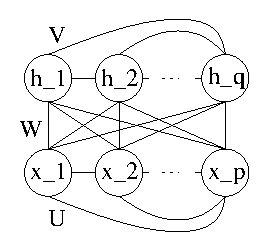
\includegraphics[width=0.4\columnwidth]{figures/fbm.eps}
    \caption{Fully-Connected Boltzmann machine.}
    \label{fig:fbm}
\end{wrapfigure}
%\end{figure}

Regardless of whether it is visible or hidden, each unit
$x_i$ is binary (having either $0$ or $1$ as its state) and
has a bias $b_i$.  Each pair $x_i$ and $x_j$ is connected by
an undirected edge with its weight $w_{ij}$, or one may say
that there are two directed edges from $x_i$ to $x_j$ and
from $x_j$ to $x_i$ with a symmetric weight $w_{ij}$. 

Let us denote the weights of the edges connecting 
the visible and hidden units, of those among the visible
units, and of those among the hidden units by $\mW \in
\RR^{p \times q}$, $\mU \in \RR^{p \times p}$ and $\mV \in
\RR^{q \times q}$, respectively. Then, as we did with both the Hopfield network
and the fully-visible Boltzmann machine previously, we define
the negative energy of the network by
\begin{align}
    \label{eq:bm_energy}
    -E(\vx, \vh \mid \TT) = \vb^\top \vx + \vc^\top \vh +
    \vx^\top \mW \vh + \frac{1}{2} \vx^\top \mU \vx +
    \frac{1}{2} \vh^\top \mV \vh,
\end{align}
where $\vb$ and $\vc$ are vectors of the biases to the
visible and hidden units, respectively. $\TT$ indicates the
set of all parameters including $\vb$, $\vc$, $\mW$, $\mU$
and $\mV$. Naturally, we define a probability of a state
$\left[ \vx^\top, \vh^\top \right]^\top$ with the Boltzmann
distribution by
\begin{align}
    \label{eq:bm_prob}
    p(\vx, \vh \mid \TT) = \frac{1}{Z(\TT)} \exp \left\{
    -E\left(\vx , \vh \mid \TT\right)
    \right\},
\end{align}
where again $Z(\TT)$ is a normalization constant that
requires the summation over an exponential number of terms
with respect to the number of units.

See Fig.~\ref{fig:fbm} for the illustration of this
Boltzmann machine.

When it comes to estimating parameters, however, the marginal
log-likelihood needs to be maximized instead. The marginal
log-likelihood is computed by marginalizing out the hidden
units:
\begin{align}
    \label{eq:bm_mll}
    \LL(\TT) =& \frac{1}{N} \sum_{n=1}^N \log \sum_{\vh}
    \exp\left(-E\left( \vx^{(n)}, \vh \mid \TT\right)\right)
    \nonumber
    \\
    &\phantom{\frac{1}{N}}- \log Z(\TT).
\end{align}

The parameters can be estimated by maximizing
Eq.~\eqref{eq:bm_mll} using, for instance, the stochastic
gradient  algorithm. This algorithm will take a small step
in the direction of the steepest ascent direction in the
parameter space. The steepest direction is computed for each
parameter by the partial derivative of the marginal
log-likelihood with respect to it. The partial derivative
with respect to a parameter $\theta$ is 
\begin{align}
    \label{eq:bm_grad}
    \frac{\partial \LL(\TT)}{\partial \theta} \propto
    \left< \frac{\partial
    \left(-E(\vx, \vh\mid\TT)\right)}{\partial \theta}
    \right>_{p\left(\vh \mid \vx,
    \TT\right)p_D\left(\vx\right) } 
    -
    \left< \frac{\partial
    \left(-E(\vx, \vh\mid\TT)\right)}{\partial \theta}
    \right>_{p\left(\vx, \vh \mid \TT\right)}.
\end{align}

The first term computes the expectation of the
partial derivative of the negative energy with respect to
the parameter under the posterior distribution of the hidden
units, with the visible units fixed to training samples from
the empirical, or data, distribution. The
second term is the expectation of the same quantity under
the model distribution represented by the Boltzmann machine.
It is obvious that computing these terms exactly is
intractable. Both terms require evaluating the
partial derivative of the negative energy exponentially many
times. 

Hence, we must resort to estimating them with various
techniques instead of trying to compute them exactly. The
first choice is to use 
samples from those intractable distributions to estimate the
statistics. The other possibility is to approximate, for
instance, the true posterior distribution over the hidden
units given the state of the visible units with a simpler
distribution. In Section~\ref{sec:estimation_bm}, we briefly
describe the underlying ideas of these two approaches and
how they can be applied to estimating parameters of a
Boltzmann machine. 

There is yet another formulation of training Boltzmann
machines that leads to exactly the same update rules in
Eq.~\eqref{eq:bm_grad}. This formulation is based on
minimizing the negative KL-divergence between the
data distribution and the model distribution, which is
defined by
\begin{align}
    \label{eq:bm_kldiv}
    -\KL(P_0 \| P_\infty) = -\sum_{\vx} \log
    \frac{P_0(\vx)}{P_\infty(\vx)} P_0(\vx) =
    \left<\log P_\infty(\vx) \right>_{P_0} - \left< \log P_0
    (\vx) \right>_{P_0},
\end{align}
where the shorthand notations $P_0$ and $P_\infty$ are,
respectively, 
defined by
\begin{align*}
    P_0 =& p\left(\vh \mid \vx, \TT\right)p_D\left(\vx\right)
    \\
    P_\infty =& p\left(\vx, \vh \mid \TT\right).
\end{align*}
A reason for this notation is related to interpolating
between the data and model distributions, which will be made
more clear in Section~\ref{sec:contrastive_divergence}. The
last term, corresponding to the entropy of the data
distribution, does not depend on the parameters $\TT$ and
can be safely ignored.

It is easy to see that Eq.~\eqref{eq:bm_kldiv} is equivalent
to Eq.~\eqref{eq:bm_mll}, since
\[
\left< \log P_\infty(\vx) \right>_{P_0} \approx \frac{1}{N}
\sum_{n=1}^N \log \sum_{\vh} p(\vx^{(n)}, \vh \mid \TT)
\]
which is exactly the marginal log-likelihood of
Eq.~\eqref{eq:bm_mll}. This fact will become useful when we
describe an efficient learning procedure, called minimizing
contrastive divergence \citep{Hinton2002}.
%, later for a
%structurally-restricted family of Boltzmann machines.

\subsection{Transformation Invariance and Enhanced Gradient}
\label{sec:enhanced_grad}

It is interesting to notice that the addition of any constant
to the energy function of a Boltzmann machine does
\textit{not} alter the probability distribution it defines
over the state space. This can be easily verified by the
fact that the new normalization constant $\tilde{Z}(\TT)$
after adding a constant to the energy is just the original
normalization constant $Z(\TT)$ multiplied by the exponential
function of the added constant, assuming that the constant
is independent of the states of both $\vx$ and $\vh$:
\begin{align*}
    \tilde{Z}(\TT) &= \sum_\vx \sum_\vh \exp\left\{
    -E(\vx, \vh \mid \TT) + C \right\} \\
    &= \exp\left\{ C \right\} \sum_\vx \sum_\vh \exp\left\{
    -E(\vx, \vh \mid \TT) \right\} \\
    &= \exp\left\{ C \right\} Z(\TT).
\end{align*}

With this property in mind, we may now investigate a
case where the states of some units are transformed. To make
equations uncluttered, in this section, we do not
distinguish between visible and hidden units, and use $\vx$
to denote all units. Also, instead of $p+q$ units, we will
use $p$ solely to indicate the number of units.

A bit-flipping transformation $\tilde{x}_i$ of unit $x_i
\in \left\{ 0, 1\right\}$ is defined by an indicator
variable $f_i \in \left\{ 0, 1\right\}$ such that 
\begin{align*}
    \tilde{x}_i = x_i^{1 - f_i} \left( 1 - x_i\right)^{f_i}.
\end{align*}
In other words, the $i$-th unit of a Boltzmann machine is
\textit{flipped}, if $f_i$ is set to $1$. Given the states
$\vx$ of the units, the bit-flipping transformation by $\vf$
results in $\tilde{\vx}$.

Let us assume that we are given a Boltzmann machine $\BB(0)$
with the parameters $\TT$. It was shown by \citet{Cho2013nc}
that there exists a Boltzmann machine $\BB(\vf)$
parameterized by $\tilde{\TT}$ that assigns the probability
to the state $\tilde{\vx}$ transformed by $\vf$ which is
equivalent to the probability assigned by the Boltzmann
machine $\BB(0)$ to the original state $\vx$. In other words,
\begin{align*}
    E(\tilde{\vx} \mid \tilde{\TT})  = E(\vx \mid \TT) + C,
\end{align*}
with the following re-parameterization:
\begin{align}
     \label{eq:bm_tilde_w}
     \tilde{w}_{ij} &= (-1)^{f_i+f_j}w_{ij},
 \\
     \label{eq:bm_tilde_b}
     \tilde{b}_i &= (-1)^{f_i}\biggl(b_i + \sum_j f_j w_{ij}
     \biggr).
\end{align}

A direct implication of this transformation-invariance
property is that learning parameters by maximizing the
log-likelihood in Eq.~\eqref{eq:bm_mll} is dependent on the
data representation. In other words, completely different
behaviors will be observed when training a Boltzmann machine
on the same data, however, with different representations.
Especially, in \citepub{Cho2013nc} it is empirically shown that
certain representations of the same dataset are favored over
other representations. For instance, a sparse data set can
easily be learned by a Boltzmann machine with the stochastic
gradient method, while its inverted form, a dense version of
the same data, cannot be learned as easily.

This phenomenon becomes more clear, if we understand that
there are exponentially many possible update directions each
time with respect to the number of units. In fact, if a
transformation is chosen to be other than the bit-flipping
transformation, there are potentially infinitely many update
directions available, as will be discussed later.

With a given bit-flipping transformation $\vf$, we first
\textit{transform} the Boltzmann machine according to
Eqs.~\eqref{eq:bm_tilde_w}--\eqref{eq:bm_tilde_b}. The
transformed model is \textit{updated} by one step of the
stochastic gradient method, and then, is \textit{transformed
back}. A simple illustration of how this three-step update
is performed is given in
Fig.~\ref{fig:bm_three_step_update}.

\begin{figure}[t]
    \centering
    \psfrag{x_1}[Bc][Bc][1][0]{$x_1$}
    \psfrag{h_1}[Bc][Bc][1][0]{$h_1$}
    \psfrag{x_2}[Bc][Bc][1][0]{$x_2$}
    \psfrag{h_2}[Bc][Bc][1][0]{$h_2$}
    \psfrag{x_p}[Bc][Bc][1][0]{$x_p$}
    \psfrag{h_q}[Bc][Bc][1][0]{$h_q$}
    \psfrag{f_1}[Bc][Bc][1][0]{$\tilde{x}_1$}
    \psfrag{g_1}[Bc][Bc][1][0]{$\tilde{h}_1$}
    \psfrag{f_2}[Bc][Bc][1][0]{$\tilde{x}_2$}
    \psfrag{g_2}[Bc][Bc][1][0]{$\tilde{h}_2$}
    \psfrag{f_p}[Bc][Bc][1][0]{$\tilde{x}_p$}
    \psfrag{g_q}[Bc][Bc][1][0]{$\tilde{h}_q$}
    \psfrag{U}[Bc][Bc][1][0]{$\mU$}
    \psfrag{W}[Bc][Bc][1][0]{$\mW$}
    \psfrag{V}[Bc][Bc][1][0]{$\mV$}
    \psfrag{U1}[Br][Bc][1][0]{$\mU+\Delta_\vf \mU$}
    \psfrag{W1}[Br][Bc][1][0]{$\mW+\Delta_\vf \mW$}
    \psfrag{V1}[Br][Bc][1][0]{$\mV+\Delta_\vf \mV$}
    \psfrag{tU}[Bc][Bc][1][0]{$\tilde{\mU}$}
    \psfrag{tW}[Bc][Bc][1][0]{$\tilde{\mW}$}
    \psfrag{tV}[Bc][Bc][1][0]{$\tilde{\mV}$}
    \psfrag{tU1}[Br][Bc][1][0]{$\tilde{\mU}+\Delta\tilde{\mU}$}
    \psfrag{tW1}[Bl][Bc][1][0]{$\tilde{\mW}+\Delta\tilde{\mW}$}
    \psfrag{tV1}[Br][Bc][1][0]{$\tilde{\mV}+\Delta\tilde{\mV}$}
    \psfrag{update}[Bc][Bc][1.2][0]{(2) Update}
    \psfrag{f}[Bl][Bl][1.2][0]{(1) Transform}
    \psfrag{finv}[Bl][Bl][1.2][0]{(3) Transform Back}
    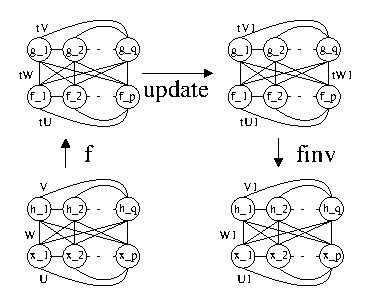
\includegraphics[width=0.8\columnwidth]{figures/fbm_3step.eps}
    \caption{Illustration of the three-step update procedure
    consisting of (1) transforming, (2) updating and (3)
    transforming back. $\Delta_\vf \TT$ denotes the change
    in $\TT$ dependent on the transformation $\vf$.}
    \label{fig:bm_three_step_update}
\end{figure}

Interestingly, this approach results in a valid
steepest-ascent update rule for each parameter that
\textit{depends on} the transformation $\vf$:
\begin{align}
  w_{ij} &\leftarrow  w_{ij} + \eta
  \left[\cov_\td(x_i,x_j)-\cov_\tf(x_i,x_j) + \right.
  \nonumber \\
  &\phantom{\leftarrow w_{ij} + \eta
  \left[\right]}\left.\left(\left<x_i\right>_\tdf-f_i\right)
  \nabla b_j + \left(\left<x_j\right>_\tdf-f_j\right) \nabla
  b_i \right], 
\label{eq:threestepW}
\\
 b_i &\leftarrow  b_i + \eta\left( \nabla b_i - \sum_j f_j \nabla_\vf
      w_{ij} \right),
\label{eq:threestepb}
\end{align}
where we used the following shorthand notations
\begin{align*}
\nabla_\vf w_{ij} &= \left<x_ix_j\right>_\td -
\left<x_ix_j\right>_\tf - f_i\nabla b_j - f_j \nabla b_i, \\
\left< x_i \right>_{\tdf} &= \frac{1}{2} \left( \left< x_i
\right>_{\td} + \left< x_i \right>_{\tf} \right),
\end{align*}
and the covariance between two units with respect to the
distribution $P$ is defined by
\begin{align*}
  \cov_P\left(x_i, h_j\right) &= \qexp{x_i h_j}_P
   -\qexp{x_i}_P \qexp{h_j}_P.
\end{align*}
As defined earlier in Section~\ref{sec:fvbm}, $\td$ and
$\tf$ correspond to the data and model distributions,
respectively. 

All these $2^p$ update directions, in the case of
the bit-flipping transformation, are valid so that they will
increase the log-likelihood. However, it may not be the case
that all such directions will lead to the same solution,
considering that the log-likelihood function in
Eq.~\eqref{eq:bm_mll} is a highly non-concave function. For
instance, one direction may lead to the solution that is
superior, in terms of log-probabilities of test samples, to
those solutions reached by other update directions.

To alleviate this problem, the author of this thesis
together with two co-authors, in \citepub{Cho2013nc} and
\citepub{Cho2011icml}, proposed to use the weighted sum of
all those directions. We define the weight $\gamma_{\vf}$ of
each gradient update dependent on the transformation $\vf$
by
\begin{align*}
    \gamma_{\vf}  = \prod_{i=1}^p \left< x_i
    \right>_{\tdf}^{f_i} \left(1 - \left< x_i
    \right>_{\tdf}\right)^{1 - f_i},
\end{align*}
where 
\[
\left< x_i \right>_{\tdf} = \frac{1}{2} \left( \left< x_i
\right>_{\td} + \left< x_i \right>_{\tf}\right).
\]

The weighted sum of exponentially many
transformation-dependent update directions, called the
enhanced gradient, is then
\begin{align}
    \label{eq:enh_w}
  \nabla_e w_{ij} &=  \cov_\td(x_i,x_j)-\cov_\tf(x_i,x_j),
  \\
    \label{eq:enh_b}
  \nabla_e b_i &= \nabla b_i - \sum_j
  \left<x_j\right>_\tdf\nabla_e w_{ij},
\end{align}
where we use $\nabla_e$ to distinguish the enhanced gradient
from the conventional gradient. It must be noticed that the
enhanced gradient is \textit{not} dependent on the
transformation $\vf$, making it invariant to the
bit-flipping transformation.

Empirical evidence has been provided in \citepub{Cho2013nc}
that the enhanced gradient is more robust to the choice of
hyper-parameters, such as a learning rate and its
scheduling, and extracts more discriminative features, when
used for training a restricted Boltzmann machine. A
restricted Boltzmann machine, which is a
structurally-restricted variant of a Boltzmann machine, will
be discussed in detail later.

%A bit-flipping transformation is just one of many possible
%transformations. 
The bit-flipping transformation introduced in
\citepub{Cho2013nc} and \citepub{Cho2011icml} have inspired
others since.  For instance, \citet{Montavon2012} showed
that centering each unit helps avoiding a difficulty in
training a deep Boltzmann machine which is another
structurally-restricted variant of a Boltzmann machine.
Instead of the bit-flipping transformation, they used a
shifting transformation such that
\begin{align*}
    \tilde{x}_i  = x_i - \beta_i.
\end{align*}
\citet{Cho2011dlufl}, which was recently published as
\citepub{Cho2013ijcnn}, also proposed independently the same
transformation for Gaussian visible units.

With the shifting transformation $\vbeta$, one can construct
the equivalent Boltzmann machine with the following
parameters
\begin{align*}
    \tilde{w}_{ij} &= w_{ij} \\
    \tilde{b}_i &= b_i + \sum_{j} w_{ij} \beta_j.
\end{align*}
However, in this case, there are \textit{infinitely} many
possible update directions at a time, and one needs to
choose a single update direction, where 
\[
\beta_i = \left< x_i \right>_\tdf
\]
was proposed in \citepub{Cho2013ijcnn}, and 
\citet{Montavon2012}
proposed to use 
\[
\beta_i = \left< x_i \right>_\td.
\]
A similar idea was also proposed by \citet{Tang2011}, but
they applied the transformation only to visible units.

\section{Boltzmann Machines with Hidden Units are Deep}

Before discussing Boltzmann machines further, in this
section, we first provide an intuitive explanation as to why
Boltzmann machines, especially with hidden units, are
considered deep. This is done by showing that a recurrent
neural network, after being unfolded over time, is deep and
an equivalent recurrent neural network can be constructed
for each Boltzmann machine.

A recurrent neural network consists of input, output and
hidden units as usual with any other types of neural
networks considered so far in this thesis. It, however,
differs from, for instance, a multilayer perceptron
introduced earlier in that there exist \textit{feed-back}
edges. Hence, a state $\left[ \vx^\top_{\qt{t}},
\vh^\top_{\qt{t}}\right]^\top$ of the network at time $t$ does not
only depend on the given input $\vx_{\qt{t}}$, but it also
depends on
the state $\left[ \vx^\top_{\qt{t-1}}, \vh^\top_{\qt{t-1}}\right]^\top$
of the units at the previous time step $t-1$. More
comprehensive discussions on general recurrent neural
networks and recent advances in their learning algorithms can
be found in
\citep[][]{Bengio2013rec,Sutskever2013,Graves2013}.

In this section, we first discuss why a recurrent neural
network with hidden units is \textit{deep}. Then, we
describe how a Boltzmann machine with hidden units may be
considered a recurrent neural network. Based on these
observations, we conclude that Boltzmann machines with
hidden units are \textit{deep} neural networks.

%It is trivial to see that a fully-visible Boltzmann machine
%or a Hopfield network is a recurrent neural network
%\citep[see, e.g.,][]{Mackay2002} without any output or
%hidden unit.  The current state of each unit $x_i(t) \in
%\left\{ 0, 1\right\}$ at time $t$ is, in the case of a
%fully-visible Boltzmann machine, decided by the probability
%computed from the states $\vx_{-i}(t-1)$ of the all other
%units at time $t-1$ according to Eq.~\eqref{eq:bm_cond}.

\subsection{Recurrent Neural Networks with Hidden Units are
Deep}
\label{sec:rnn_deep}

Let us start with a simplified recurrent neural network
consisting of an input layer, a single nonlinear hidden
layer and a output layer. Each hidden layer receives signal
from the hidden layer at the previous time $t-1$. The set
$\TT$ of parameters consists of weights from the input layer
to the hidden layer ($\mW$), those from the hidden layer to
the output layer ($\mU$) and those from the previous hidden
layer to the current hidden layer ($\mG$).  Every unit has
its own bias term. See Fig.~\ref{fig:rnn}(a) for the
illustration of this network.

\begin{figure}[t]
    \begin{minipage}{0.40\textwidth}
        \centering
        \psfrag{W}[Bc][Bc][1][0]{$\mW$}
        \psfrag{U}[Bc][Bc][1][0]{$\mU$}
        \psfrag{G}[Bc][Bc][1][0]{$\mG$}
        \psfrag{Gt}[Cc][Cc][1][0]{}
        \psfrag{x}[Bc][Bc][1][0]{$\vx$}
        \psfrag{h}[Cc][Cc][1][0]{$\vh$}
        \psfrag{y}[Cc][Cc][1][0]{$\vy$}
        \psfrag{z}[Cc][Cc][0.8][0]{$\text{z}^{-1}$}
        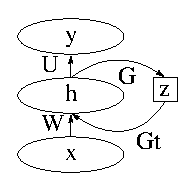
\includegraphics[width=0.65\columnwidth]{figures/rnn.eps}
    \end{minipage}
    \begin{minipage}{0.58\textwidth}
        \centering
        \psfrag{x_1}[Bc][Bc][1][0]{$\vx^{\qt{1}}$}
        \psfrag{y_1}[Bc][Bc][1][0]{$\vy^{\qt{1}}$}
        \psfrag{h_1}[Bc][Bc][1][0]{$\vh^{\qt{1}}$}
        \psfrag{x_2}[Bc][Bc][1][0]{$\vx^{\qt{2}}$}
        \psfrag{y_2}[Bc][Bc][1][0]{$\vy^{\qt{2}}$}
        \psfrag{h_2}[Bc][Bc][1][0]{$\vh^{\qt{2}}$}
        \psfrag{x_3}[Bc][Bc][1][0]{$\vx^{\qt{3}}$}
        \psfrag{x_4}[Bc][Bc][1][0]{$\vx^{\qt{4}}$}
        \psfrag{y_3}[Bc][Bc][1][0]{$\vy^{\qt{3}}$}
        \psfrag{h_3}[Bc][Bc][1][0]{$\vh^{\qt{3}}$}
        \psfrag{h_0}[Bc][Bc][1][0]{$\vh^{\qt{0}}$}
        \psfrag{G}[Bc][Bc][1][0]{$\mG$}
        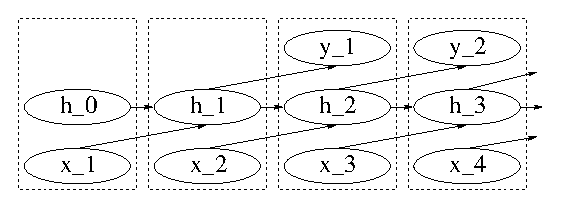
\includegraphics[width=\columnwidth]{figures/rnn_tf.eps}
    \end{minipage}

    \vspace{2mm}
    \begin{minipage}{0.48\textwidth}
        \centering
        \small
        (a) Recurrent Neural Network
    \end{minipage}
    \begin{minipage}{0.48\textwidth}
        \centering
        \small
        (b) Unfolded over Time
    \end{minipage}
    \caption{(a) A simple recurrent neural network.
    $\text{z}^{-1}$ is a unit delay operator. (b) The same
    recurrent neural network has been unfolded over time.
    Each layer is grouped by a rectangle with dashed lines.}
    \label{fig:rnn}
\end{figure}

The goal of this network is to learn to predict a sequence
of labels, given a sequence of input vectors. It is also
possible to train it to predict the next input given the
sequence of previous inputs. For instance,
\citet{Sutskever2011} showed that a recurrent neural network
was able to learn and generate an arbitrary sequence of text
once the network was trained this way.

Now, let us unfold the described recurrent neural network in
time, starting from $t = 0$, assuming that the
activations of the input and hidden units are fixed to zero
initially. We will try to construct a deep
multilayer perceptron (MLP) from the unfolded recurrent
neural network.

If we denote the input, output and hidden layers of the
recurrent neural network at time $t$ by $\vx^{\qt{t}}$,
$\vy^{\qt{t}}$ and
$\vh^{\qt{t}}$, the $l$-th layer of the infinite-depth MLP is
constructed by concatenating $\vx^{\qt{t}}$, $\vy^{\qt{t-2}}$ and
$\vh^{\qt{t-1}}$. Then, each consecutive intermediate layers $t$
and $t+1$ are connected by a sparse weight matrix, where the
connections from $\vy^{\qt{t-2}}$ to $\vh^{\qt{t}}$ and from
$\vh^{\qt{t-1}}$ to $\vx^{\qt{t+1}}$ are \textit{not} present, but
both $\vh^{\qt{t-1}}$ to $\vh^{\qt{t}}$ ($\mG$) and to
$\vy^{\qt{t-1}}$
($\mU$) and $\vx^{\qt{t}}$ to $\vh^{\qt{t}}$ ($\mW$) are. In this MLP,
unlike how MLPs were described in Section~\ref{sec:mlp}
earlier, not only the bottom-most and top-most layers, but
all intermediate layers also have input and output units,
and this network shares the weights parameters of each
layer.  See Fig.~\ref{fig:rnn}(b) for the structure of this
unfolded network.

This unfolded recurrent neural network satisfies, like a
plain MLP, the two conditions described in
Section~\ref{sec:deep_conditions} in a non-trivial way. 

First, the network can be easily extended, just like an MLP,
by adding one or more hidden layers. However, in the case of
a recurrent neural network, this addition grows the size of
each layer instead of the number of layers, when viewed as
the time-unfolded network. This is an obvious consequence
from the fact that potentially the time-unfolded network
already has infinitely many layers.

%First, the network can be easily extended by simply
%lengthening the training sequences. In fact, when the
%network is given a novel sample, it can be used to predict
%as long a sequence as one wants by continuing the
%feedforward propagation. Though, this continued
%feedforward propagation is not guaranteed to work well if
%the number of time steps taken becomes larger than the
%training sequences. However, it should be noticed that a
%fully-visible Boltzmann machine does \textit{not} satisfy
%this condition, as there is no layer having \textit{hidden}
%units in the unfolded network.

The second condition is trivially satisfied as each layer is
parameterized. One can modify the backpropagation algorithm
(see Section~\ref{sec:backprop}) used for training
conventional MLPs to train all the parameters.

Hence, we consider any recurrent neural network with hidden
units a \textit{deep} neural network. 
%This automatically
%justifies classifying any Boltzmann machine with hidden
%units into a deep neural network.

\subsection{Boltzmann Machines are Recurrent Neural Networks}

Similarly, let us consider a fully-connected Boltzmann
machine (BM) trained on a training set consisting of vectors
of samples augmented by their labels. Each label is
considered to be transformed into a binary vector using a
$1$-of-$K$ coding.  That is, the visible units are divided
into those $\vx$ that correspond to input components and
those $\vy$ that correspond to label components\footnote{ 
A practical description of how a
Boltzmann machine trained on samples augmented with their
labels will be presented in more detail in Section~\ref{sec:drbm}.
Here, this model is only used to illustrate how
an equivalent recurrent neural network can be built for a Boltzmann
machine.
}.
Furthermore, let us assume that there is no edge between the
sets of the input and label units and also no edge inside
those sets. Then, we may rewrite the energy function of the
BM in Eq.~\eqref{eq:bm_energy} into
\begin{align}
    \label{eq:disbm_energy}
    -E(\vx, \vy, \vh \mid \TT) = \va^\top \vx + \vb^\top \vy
    + \vc^\top \vh + \vx^\top \mW \vh + \vy^\top \mU +
    \frac{1}{2} \vh^\top \mV \vh.
\end{align}

Once the BM is trained, we can obtain a sequence $\left(
\vy_{\qt{0}}, \vy_{\qt{1}}, \dots, \vy_{\qt{\infty}} \right)$ of
vectors of the states of label units given a visible sample
by simulating the Boltzmann machine.  To do so, at each time
$t$, we need to have the previous states of the hidden units
$\vh_{\qt{t-1}}$ and label units $\vy_{\qt{t-1}}$. 

Given these previous states, we first compute the states of
the hidden units at time $t$ by replacing \textit{one} unit.
The state of the unit $h_{j_t}$ can be sampled from
\[
p(h_{j_t} = 1 \mid \vx, \vy_{\qt{t-1}}, \vh_{\qt{t-1}}, \TT) = \phi\left( 
\sum_{i} w_{i{j_t}} x_{i} 
+ \sum_{l} u_{l{j_t}} y'_{l} 
+ \sum_{k \neq {j_t}} v_{k{j_t}} h'_k 
+ b_{j_t} \right),
\]
where $y'_l$ and $h'_k$ are the $l$-th component of
$\vy_{\qt{t-1}}$ and the $k$-th component of $\vh_{\qt{t-1}}$,
respectively. Subsequently with the new hidden state
$\vh_{\qt{t}}$, we replace a \textit{single} unit $y_{l_t}$ to
get the new label state $\vy_{\qt{t}}$ similarly by sampling
from
\[
p(y_{l_t} = 1 \mid \vx, \vy_{\qt{t-1}}, \vh_{\qt{t}}, \TT) = \phi\left( 
\sum_{i} w_{i{j_t}} x_{i} 
+ \sum_{k \neq l_t} u_{k{l_t}} y'_{k} 
+ \sum_{j} v_{lj} h'_j 
+ a_{l_t} \right).
\]
The indices $j_t$ and $l_t$ may be chosen arbitrarily at
each time $t$. 

\begin{figure}[t]
    \begin{minipage}{0.40\textwidth}
        \centering
        \psfrag{W}[Bc][Bc][1][0]{$\mW$}
        \psfrag{U}[Bc][Bc][1][0]{$\mU$}
        \psfrag{0}[Bc][Bc][1][0]{$\mzero$}
        \psfrag{x}[Bc][Bc][1][0]{$\vx$}
        \psfrag{h}[Cc][Cc][1][0]{$\vh$}
        \psfrag{y}[Cc][Cc][1][0]{$\vy$}
        \psfrag{z}[Cc][Cc][0.8][0]{$\text{z}^{-1}$}
        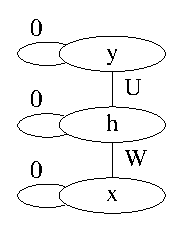
\includegraphics[width=0.65\columnwidth]{figures/bm_rnn_orig.eps}
    \end{minipage}
    \begin{minipage}{0.58\textwidth}
        \centering
        \psfrag{x}[Bc][Bc][1][0]{$\vx$}
        \psfrag{y_1}[Bc][Bc][1][0]{$\vy^{1}$}
        \psfrag{h_1}[Bc][Bc][1][0]{$\vh^{1}$}
        \psfrag{x_2}[Bc][Bc][1][0]{$\vx^{2}$}
        \psfrag{y_2}[Bc][Bc][1][0]{$\vy^{2}$}
        \psfrag{h_2}[Bc][Bc][1][0]{$\vh^{2}$}
        \psfrag{x_3}[Bc][Bc][1][0]{$\vx^{3}$}
        \psfrag{x_4}[Bc][Bc][1][0]{$\vx^{4}$}
        \psfrag{y_3}[Bc][Bc][1][0]{$\vy^{3}$}
        \psfrag{h_3}[Bc][Bc][1][0]{$\vh^{3}$}
        \psfrag{h_0}[Bc][Bc][1][0]{$\vh^{0}$}
        \psfrag{y_0}[Bc][Bc][1][0]{$\vy^{0}$}
        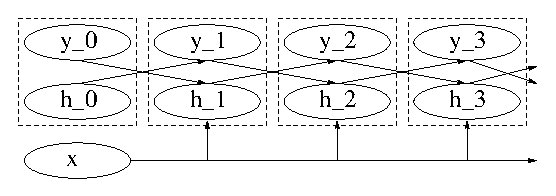
\includegraphics[width=\columnwidth]{figures/bm_rnn.eps}
    \end{minipage}

    \vspace{2mm}
    \begin{minipage}{0.48\textwidth}
        \centering
        \small
        (a) Original Boltzmann Machine
    \end{minipage}
    \begin{minipage}{0.48\textwidth}
        \centering
        \small
        (b) Equivalent Recurrent Neural Network
    \end{minipage}
    \caption{(a) A Boltzmann machine with some edges fixed
    to $0$ having visible units that correspond to a label.
    (b) The equivalent recurrent neural network unfolded over
    time. Each layer is grouped by a rectangle with dashed
    lines.}
    \label{fig:bm_rnn}
\end{figure}

It is easy to see that this way of viewing the simulation of
the BM is equivalent to performing a feedforward pass
through time in a recurrent neural network. One difference
to the recurrent neural network described in
Section~\ref{sec:rnn_deep} is that the visible units are
fixed to a sample over time. 

Also, it is obvious that there are multiple computation
paths from the visible units via both the hidden and label
units to the label units at some time $t > 1$. Furthermore,
all the parameters in the BM, or in the equivalent recurrent
neural network, are trainable in the sense that they are
estimated by maximizing the marginal log-likelihood in
Eq.~\eqref{eq:bm_mll}. Based on these observations, we
can consider Boltzmann machines with hidden units
as \textit{deep}.

In Fig.~\ref{fig:bm_rnn}, an illustration of a Boltzmann
machine with label units and its equivalent time-unfolded
recurrent neural network is shown. Note that for
simplicity in the figure we further assumed that there is
no edge among hidden units.


\section{Estimating Statistics and Parameters of Boltzmann
Machines}
\label{sec:estimation_bm}

In order to compute the gradient of the marginal
log-likelihood of a fully-connected Boltzmann machine in
Eq.~\eqref{eq:bm_mll}, we must be able to compute the
statistics under the following intractable
distributions\footnote{Here we say that a distribution is
\textit{intractable}, when there is no explicit analytical
form of the probability mass/density function available, or
the statistics of the distribution cannot be computed
analytically.}:
\begin{enumerate}
    \itemsep 0em
    \item $p(\vh \mid \vx, \TT)$: the posterior distribution
        of $\vh$ with the fixed state of $\vx$
    \item $p(\vx, \vh \mid \TT)$: the joint distribution
        modeled by the Boltzmann machine
\end{enumerate}

In this section, we briefly discuss two approaches that can
be used to compute the statistics under these distributions
approximately.

\subsection{Markov Chain Monte Carlo Methods for Boltzmann
Machines}
\label{sec:mcmc}

When one considers estimating the expectation of a function
$f$ over a distribution $\tilde{p}$, the most obvious approach one
can think of is to collect a large number of samples from
the distribution and use them to compute $f$, such that
\begin{align*}
    \E_{\tilde{p}(\vx)} \left[ f(\vx) \right] = \sum_{\vx} f(\vx)
    \tilde{p}(\vx) \approx \frac{1}{T} \sum_{t=1}^T
    f(\vx_{\qt{t}}),
\end{align*}
where $\left\{ \vx_{\qt{t}} \right\}_{t=1}^T$ is a set of $T$
samples collected from $\tilde{p}$. This effectively reduces the
problem of computing the statistics of an intractable
distribution to the problem of collecting samples from the
distribution.

A Markov Chain Monte Carlo (MCMC) method is a general
framework on which sequential sampling can be built to
collect samples from a distribution \citep[see, e.g.,][for
comprehensive review on using MCMC sampling in probabilistic
models]{Neal1993,Mackay2002}. This method is based on the idea that
sampling from a target distribution is equivalent to
simulating a \textit{Markov chain} which has the target
distribution as its unique stationary distribution.

A Markov chain consists of a set of states, for instance,
all possible states of the units of a Boltzmann machines
$\left\{ \vx \right\}$, and a transition probability
$\T(\tilde{\vx} \mid \vx)$ of the new state $\tilde{\vx}$
from the current state $\vx$ which only depends on the
current state. Given a probability distribution $p^{\qt{t}}$
over the states at time $t$, the probability distribution
$p^{\qt{t+1}}$ can be fully specified by
\begin{align*}
    p^{\qt{t+1}}(\vx) = \sum_{\tilde{\vx}} p^{\qt{t}}(\tilde{\vx})
    \T(\vx \mid \tilde{\vx}).
\end{align*}

In order to be used as a sampler of a target distribution
$\tilde{p}$, the stationary distribution $p^{\qt{\infty}}$ of this
chain at the limit of $t \to \infty$ must coincide with the
target distribution $\tilde{p}$, that is,
\begin{align*}
    p^{\qt{t}}(\vx) = \tilde{p}(\vx)\text{ as }t \to \infty.
\end{align*}

The stationary distribution, or equivalently the target
distribution, must be invariant with respect to the chain.
In other words, any further simulation of the Markov chain
does not alter the distribution of the states once the
stationary distribution has been reached. That is,
\begin{align*}
    p^{\qt{\infty}}(\vx) = \sum_{\tilde{\vx}}
    p^{\qt{\infty}}(\tilde{\vx}) \T(\vx \mid \tilde{\vx}).
\end{align*}
Due to this property of invariance, the stationary
distribution is often referred to as the \textit{equilibrium
distribution}.

This condition of invariance is usually met by designing a
transition probability, or operator, $\T$ to satisfy 
detailed balance:
\begin{align*}
    \T(\vx_0 \mid \vx_1)\tilde{p}(\vx_1) = \T(\vx_1 \mid
    \vx_0)\tilde{p}(\vx_0),
\end{align*}
for arbitrary $\vx_{0}$ and $\vx_{1}$.  Satisfying this
implies that the target distribution $\tilde{p}$ is
invariant under the Markov chain.

Furthermore, the chain must be ergodic, which implies that
the stationary distribution is reachable
regardless of the initial distribution $p^{\qt{0}}$:
\begin{align}
    \label{eq:mcmc_ergodic}
    p^{\qt{t}}(\vx) = \tilde{p}(\vx)\text{ as }t \to
    \infty\text{, }\forall p^{\qt{0}}.
\end{align}
Intuitively, it will be impossible to use the chain to
collect samples from a target distribution, if the
simulation of the chain converges to one or more
distributions that are \textit{not} the target distribution,
depending on the initial distribution.

Using this property, we can use a Markov chain to collect
samples from a target distribution. We start with an initial
distribution which usually gives to a single state the whole
probability mass ($=1$) and all the others zero probability. Because the
chain is ergodic, the simulation of the chain will
eventually end up in the stationary distribution which is
equivalent to the target distribution. From there on, we
record the sequence of states the simulation visits. The
invariance of the distribution on the chain ensures that the
state transitions, or simulation, will not move away from
the stationary distribution. The recorded list of states
will be the samples from the target distribution, albeit not
necessarily independent samples.

One representative example of MCMC methods is
the Metropolis-Hastings method \citep{Hastings1970}. In the
Metropolis-Hastings method, we assume that the target
distribution is computable up to the normalization constant,
and introduce a proposal distribution $Q$ from which we can
readily and efficiently sample.

Let us define a transition probability $\T$ as
\begin{align*}
    \T(\tilde{\vx} \mid \vx) = Q(\tilde{\vx}\mid \vx)
    \alpha(\tilde{\vx}, \vx),
\end{align*}
where the acceptance probability $\alpha(\tilde{\vx}, \vx)$ is
defined as
\begin{align}
    \label{eq:accept_prob}
    \alpha(\tilde{\vx}, \vx) = \min \left(1, 
    \frac{p^*(\tilde{\vx})Q(\vx \mid \tilde{\vx})}
    {p^*(\vx)Q(\tilde{\vx} \mid \vx)} \right).
\end{align}
We used $p^*$ to denote an unnormalized probability
such that
$\tilde{p}(\vx) = \tfrac{p^*(\vx)}{\int p^*(\vx') \dd{\vx'}}$.

\begin{algorithm}[tb]
    \caption[Metropolis-Hastings
    Method]{Metropolis-Hastings}
    \label{alg:mh}
    \begin{algorithmic}
        \STATE Initial state $\vx_{\qt{0}}$, the proposal
        distribution $Q$, the unnormalized distribution
        $p^*$ and the maximum number $M$ of proposal are required.

        \STATE Create an empty set of samples $\boldsymbol{X}=\{\}$.

        \FOR{$t=1, \cdots, M$}
        \STATE Sample $\vx'$ from $Q(\vx \mid
        \vx_{\qt{t-1}})$.
        \STATE Compute the acceptance probability
        $\alpha$ using Eq.~\eqref{eq:accept_prob}.
        \STATE Draw a sample $s$ from the uniform distribution
        $\mathcal{U}(0, 1)$.
        \IF{$s < \alpha$}
        \STATE Add $\vx'$ to $\boldsymbol{X}$.
        \STATE Set $\vx_{\qt{t}} = \vx'$.
        \ENDIF
        \ENDFOR
        \STATE
        $\boldsymbol{X}$ is the set of samples collected by
        Metropolis-Hastings method.
    \end{algorithmic}
\end{algorithm}

With this, we can sample from the target
distribution $\tilde{p}$ following the procedure described
in Alg.~\ref{alg:mh}.
%\begin{itemize}
%    \itemsep 0em
%    \item[(Proposal)] Sample $\vx'$ from $Q(\vx \mid
%        \vx_{\qt{t}})$
%    \item[(Acceptance)] ~\\ 
%        (Accept) Set $\vx_{\qt{t+1}} = \vx'$ with the
%        probability $\alpha(\vx', \vx_{\qt{t}})$  \\
%        (Reject) Otherwise, set $\vx_{\qt{t+1}} =
%        \vx_{\qt{t}}$.
%\end{itemize}
With some mild assumptions on the proposal distribution $Q$,
the distribution of $\vx_{\qt{t}}$ will converge to the target
distribution $\tilde{p}(\vx)$ using the Metropolis-Hastings
method.

\subsubsection{Gibbs Sampling}
\label{sec:gibbs}

One particular form of the Metropolis-Hastings method is
Gibbs sampling, in which we are more interested, in the case
of Boltzmann machines. Gibbs sampling can be derived by
using the conditional distribution of a single component $k$
given the state of all other components, denoted by $-k$, as
the proposal distribution $Q$. That is,
\begin{align*}
    Q(\tilde{\vx} \mid \vx) = p(\vx_k \mid \vx_{-k}),
\end{align*}
where $\tilde{\vx}_{-k} = \vx_{-k}$.
This choice makes the acceptance probability $\alpha$ always
one so that every sample is accepted.

With this proposal distribution and the property of
accepting always, the Gibbs sampling can be implemented
simply by repeatedly collecting a new sample from
\begin{align*}
    \vx' = \left[ x_1, x_2, \cdots,
    x'_k, \cdots, x_p \right],
\end{align*}
where $x'_k$ is sampled by
\begin{align*}
    x'_k \sim x_k \mid x_1, \cdots, x_{k-1},
    x_{k+1}, \cdots, x_p,
\end{align*}
and $p$ is the dimensionality of $\vx$, while changing $k$
in a predefined schedule. It is usual to simply cycle $k$
through all the components sequentially.

Because the conditional probability of each unit in a
Boltzmann machine (Eq.~\eqref{eq:bm_cond}) is well defined
and easily evaluated, it is natural to use Gibbs
sampling to evaluate the statistics of the distributions
$p(\vh \mid \vx, \TT)$ and $p(\vx, \vh \mid \TT)$. 
%Using the
%Gibbs sampling, it is now possible to estimate, for
%instance, the gradient in Eq.~\eqref{eq:bm_grad}.

However, this sampling-based approach, especially with the
Gibbs sampling, may not be practical due to several reasons.
Firstly, it is usually difficult, if not impossible, to
determine the convergence of the Markov chain, which leaves
collecting as many samples as possible the only option.
Secondly, Gibbs sampling or any other
Metropolis-Hastings method with a local proposal
distribution in which each consecutive sampling steps can
only make a local change, will require a large amount of
steps to
explore the whole distribution, especially when there are multiple modes
in it. 

The latter issue is especially prevalent when one tries to sample
from the joint distribution $p(\vx, \vh \mid \TT)$.  The
joint distribution, and consequently the marginal
distribution of $\sum_{\vh} p(\vx, \vh \mid \TT)$, is after
all optimized to have multiple modes that correspond to,
for instance, different classes or clusters of a given
training set. Unless the training set consists of samples
from a unimodal distribution, the joint distribution $p(\vx,
\vh \mid \TT)$ that models the training set well enough will
always have more than one modes.


%\subsubsection{Other than Gibbs Sampling: Parallel Tempering}
\subsubsection{Parallel Tempering}
\label{sec:parallel_tempering}

%Although the structural restriction on an RBM enables the
%Gibbs sampling to be performed efficiently in a parallelized
%environment, the Gibbs sampling still has a problem. 

The major problem of Gibbs sampling is that it often
fails to explore isolated modes lying far away in the
distribution.  In many cases, the Gibbs sampling chain is
stuck at one mode and is unable to escape from it. In other
words, the convergence of the Gibbs chain to the stationary
distribution might take too long, or infinitely long.

In order to prevent this problem, several approaches have
been proposed to improve the mixing property of Gibbs
sampling in collecting samples from Boltzmann machines.
\citet{Salakhutdinov2009} proposed to use tempered
transitions \citep{Neal1994}, while a similar, but not
identical sampling method based on tempered chains called
parallel tempering was proposed in
\citepub{Cho2010ijcnn} and independently by
\citet{Desjardins2010,Desjardins2010a}.  Instead of
introducing a new sampling scheme, \citet{Tieleman2009}
described a method of using \textit{fast} parameters,
in the case of training restricted Boltzmann
machines.
%which will be discussed later.

Here, we will mainly discuss one of those proposed
approaches, called \textit{parallel tempering}, which was
empirically found to improve the generative performance.

Parallel tempering was introduced by \citet{Swendsen1986}
under the name of a replica Monte Carlo simulation applied
to an Ising model which is equivalent to the fully-visible
Boltzmann machine (see Section~\ref{sec:fvbm}).
\citet{Geyer1991} later presented the application of
parallel chaining of MCMC sampling based on the speed of
mixing of samples across parallel chains to the maximum
likelihood estimator.

Let us first introduce an inverse temperature $\beta$
which was assumed to be fixed to $1$ earlier for a Boltzmann
machine. The joint probability
of a Boltzmann machine of the inverse temperature $\beta$ is defined by
\begin{align*}
    p_{\beta} (\vx, \vh) = p (\vx, \vh \mid \TT_\beta) =
    \frac{1}{Z(\TT_\beta)} \exp\left\{ -\beta E(\vx, \vh
    \mid \TT) \right\}.
\end{align*}
Let us call the distribution represented by the Boltzmann
machine with the inverse temperature $\beta$ a
\textit{tempered distribution} with $\beta$.

Parallel tempering can be understood as a composite of two
transition operators, if we only consider two
tempered distributions with $\beta=1$ (model distribution)
and $\beta = \beta_q < 1$ (proposal distribution) for now.  Since
the concatenation of valid MCMC transitions satisfies the
properties of a valid MCMC method, parallel tempering as a
composite of two operators is a valid MCMC method.

The first transition operator, which performs a single-step
Gibbs sampling on the model distribution, is applied to the
current sample $\vx$ and results in a new sample $\vx'$.
Then the second transition operator performs a single step
of the Metropolis-Hastings sampling from the new sample
$\vx'$.

In the second transition operator, the proposal distribution
is the tempered distribution with the inverse temperature
$\beta_q$. The sample $\vx''$ from the proposal distribution
will be obtained by yet another Gibbs sampling step on the
tempered distribution. Then, $\vx''$ is accepted with the
probability
\begin{align}
    \label{eq:pt_swap_prob}
    p_\text{swap} (\vx', \vx'') = \min \left( 1, \frac{p_1^*
    (\vx'') p^*_{\beta_q} (\vx')}{p^*_1(\vx')
    p^*_{\beta_q}(\vx'')}
    \right),
\end{align}
where $p^*$ indicates that it is an \textit{unnormalized}
probability. If accepted, we keep $\vx''$ as the new
sample and otherwise, $\vx'$ is kept.

The reason why the acceptance probability in
Eq.~\eqref{eq:pt_swap_prob} was denoted a \textit{swap}
probability is that once we switch the roles between the
model distribution and the proposal distribution, we can see
that this probability, in essence, decides whether the
samples from the two distributions be swapped or not.

Let us now assume that we have a series of $N+1$ tempered
transitions such that $\beta_0=0 < \cdots < 1 = \beta_N$.
Then we can apply the above transition operator to each
consecutive pairs of the tempered distribution. That is, 
sampling from the proposal distribution is replaced by the
same transition operator applied to the pair of tempered
distributions immediately below. This \textit{chaining}
continues down to the bottom pair.

Since the top tempered distribution with the inverse
temperature $\beta=1$ corresponds to the model distribution,
the samples that stay on it are the ones from the model
distribution. We can use them to compute the statistics of
the model distribution of a Boltzmann machine. When we use
the parallel tempering with the stochastic approximation
procedure (see Section~\ref{sec:sap}), we apply the above
transition operator a few times at each update and use the
samples from the top chain to compute the gradient while
maintaining the samples of the other chains as well.

When the inverse temperature is $0$, the tempered
distribution is completely flat, meaning that every state is
assigned the same probability $\frac{1}{2^{p+q}}$. Under
this distribution, one can draw an exact sample from the
stationary distribution without even running any MCMC
sampling chain. One can simply draw the state of each unit
from a Bernoulli random variable with its mean $0.5$. 

In other words, the tempered distributions with low
$\beta$'s tend to be smooth overall, and the Gibbs sampling
on those distributions is less prone to being trapped in a
single, or only few, modes out of all modes in the
distributions. As $\beta$ approaches $1$ (model
distribution), it becomes more difficult for the plain Gibbs
sampling to explore the whole state space efficiently.

In this regard, the obvious advantage of parallel
tempering when compared to Gibbs sampling is that 
parallel tempering can avoid being trapped in a single mode.
This is possible, since the samples from the Gibbs sampling
chains in the tempered distributions with smaller $\beta$'s
are less prone to becoming highly correlated with each other.
A sample in a lower chain, that is far away from the mode
in which the current sample at the top chain is trapped, may be
swapped to become a new sample at the top chain, and this
helps preventing having a sequence of highly correlated
samples. 

This behavior of exploring other modes easily is illustrated
in Fig.~\ref{fig:pt_escape}.

\begin{figure}[t]
    \centering
    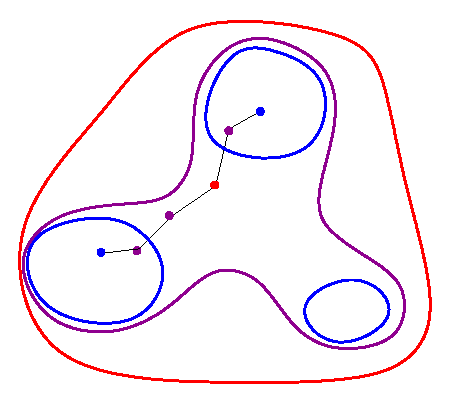
\includegraphics[width=0.45\textwidth]{figures/pt.eps}
    \caption{Illustration of how PT sampling could avoid
    being trapped in a single mode. The red, purple, and
    blue curves and dots indicate distributions and the
    samples from the distributions with the high, medium,
    and cold temperatures, respectively. Each black line
    indicates a single sampling step. Reprinted from
    \citep{Cho2011t}.}
    \label{fig:pt_escape}
\end{figure}

In \citepub{Cho2010ijcnn}, it is empirically shown that if
the same number of Gibbs steps is allowed, using parallel
tempering to compute the statistics of the model
distribution results in a better generative model compared
to the plain Gibbs sampling, when an RBM was trained.

Similarly, the tempered transition and the
coupled adaptive simulated tempering
\citep{Salakhutdinov2010} are all based on using 
tempered distributions. All these methods are superior to
the plain Gibbs sampling in the sense that the whole state
space can be explored more easily.


\subsection{Variational Approximation: Mean-Field Approach}
\label{sec:bm_vari}

A variational approximation is another way of computing the
intractable statistics of a probability distribution such as
the posterior distribution of a Boltzmann machine over its
hidden units. Here we discuss how the variational
approximation, which has already been discussed briefly
earlier in Section~\ref{sec:autoencoder_vari}, can be
applied to computing the statistics of a Boltzmann machine.

Let us start by restating how the marginal log-likelihood in
general can be decomposed into two terms, which was
presented in Eqs.~\eqref{eq:mll_decom}--\eqref{eq:mll_post}:
\begin{align}
    \label{eq:bm_vari}
    \LL(\TT) &= \LL_Q(\TT) + \KL(Q \| P) 
    \nonumber
    \\
    &\geq 
    \E_{Q} \left[ \log p(\vx, \vh \mid
    \TT)\right] + \HH(Q)
\end{align}
$Q$ and $P$ are respectively an arbitrary distribution
over hidden variables and the posterior distribution over
the hidden variables given the states of visible, or
observed, variables.

This same decomposition applies to the marginal
log-likelihood of a Boltzmann machine with hidden units
presented in Eq.~\eqref{eq:bm_mll}. In other words, we can
also in the case of Boltzmann machines maximize the
lower bound $\LL_Q(\TT)$ instead of maximizing the original
marginal log-likelihood directly.

Let us assume that we use a fully factorized distribution
$Q(\vh \mid \TT_Q)$ parameterized by $\TT_Q$. By considering
that each hidden unit can have either $0$ or $1$, we can use
the following factorized $Q$ proposed by
\citet{Salakhutdinov2009}:
\begin{align}
    \label{eq:bm_fact_q}
    Q(\vh \mid \TT_Q) = \prod_{j=1}^q q(h_j),
\end{align}
where $q(h_j = 1) = \mu_j$ and $\mu_j$'s are the parameters
of $Q$. This approach of using a fully factorized
approximate posterior is often called a mean-field approximation.

By plugging Eq.~\eqref{eq:bm_fact_q} and
Eq.~\eqref{eq:bm_prob} into Eq.~\eqref{eq:bm_vari}, we can
rewrite the lower bound $\LL_Q(\TT)$ as
\begin{align}
    \label{eq:bm_lowerbound}
    \LL_Q(\TT) =& \sum_{i=1}^p b_i x_i + \sum_{j=1}^q c_j
    \mu_j + \sum_{i=1}^p x_i \mu_j w_{ij} + 
    \nonumber \\ 
    & \sum_{i=1}^p \sum_{j=i+1}^p x_i x_j u_{ij} +
    \sum_{i=1}^q \sum_{j=i+1}^q \mu_i \mu_j v_{ij} -\log
    Z(\TT) 
    \nonumber \\
    & - \sum_{j=1}^p \left( \mu_j \log \mu_j + (1
    - \mu_j) \log (1 - \mu_j)
    \right).
\end{align}
By maximizing this with respect to $Q$, or its
parameters $\TT_Q$, we can minimize the difference between
$Q$ and the true posterior distribution. 

Maximization can be done simply by taking the
partial derivative of $\LL_Q$ with respect to each variational
parameter $\mu_j$ and updating it according to the computed
direction. By setting the partial derivative of $\LL_Q$ with
respect to $\mu_j$ to zero, we get the following fixed-point
iteration:
\begin{align}
    \label{eq:vari_update}
    \mu_j \leftarrow \phi\left(\sum_{i=1}^p w_{ij} x_i +
    \sum_{k=1, k\neq j}^q v_{kj} h_k + c_j\right),
\end{align}
where $\phi$ is a logistic sigmoid function.

Once $\TT_Q$ converges after running the fixed-point
iterations several times, we may use it not only for
estimating the parameters as a part of a problem of
maximizing the lower bound of the marginal log-likelihood,
but also as an approximate posterior distribution of a given
sample. For instance, one can use the variational parameters
$\TT_Q$ of each sample as a feature vector for another
model.

Despite its advantages, such as easy parallelization and
easy-to-check convergence, there is an important limitation
in this approach. The limitation comes from the unimodality
of the fully factorized form of the approximate posterior
distribution $Q$.

Because all hidden units were assumed to be independent from
each other, $Q$ can only have a single mode, unless
$\mu_j=0.5$ for some $j$. If the distribution approximated
by $Q$ has more than one mode, due to the property of the
KL-divergence and the order\footnote{Note that the order of
$Q$ and $P$ matters when their KL-divergence is computed, as
the KL-divergence is \textit{not} a symmetric measure.} of
$Q$ and the true distribution $P$, the approximate
distribution $Q$ will tend to approximate one of those
multiple modes in the true distribution $P$
\citep[see][Section 21.2.2 for more details]{Murphy2012}.

This especially limits using the variational approximation
for estimating the joint distribution ${p(\vx, \vh \mid
\TT)}$. As discussed earlier, it is highly likely that
${p(\vx, \vh \mid \TT)}$ will be highly multimodal as
learning continues, and the statistics estimated by the
approximate distribution will \textit{not} reflect the true
statistics well. Furthermore, in the context of Boltzmann
machines, this approximation will not work for the joint
distribution since the parameters estimated by the
gradient-based update will increase the KL-divergence
between the approximate distribution and the true joint
distribution due to the minus sign in front of $\log Z(\TT)$
in Eq.~\eqref{eq:bm_lowerbound}.

Hence, it is usual to use this variational approximation for
estimating the statistics under the posterior distribution
${p(\vh \mid \vx, \TT)}$, while an approach based on MCMC
methods is used to estimate the statistics under the joint
distribution. 
%We will discuss the actual learning algorithms
%based on these approaches later in this chapter, in more
%detail.

\subsection{Stochastic Approximation Procedure for Boltzmann Machines}
\label{sec:sap}

Using a naive stochastic gradient method described in
Section~\ref{sec:stochastic_grad}, we can find the set of
parameters that maximizes the marginal log-likelihood
\eqref{eq:bm_mll} or the variational lower bound
\eqref{eq:bm_lowerbound} of a Boltzmann machine. One can
simply repeat the following update to each parameter:
\begin{align}
    \theta^{\qt{t+1}} &= \theta^{\qt{t}} + \eta_{\qt{t}} \left( 
    \left< h(\vx, \vh\mid \TT^{\qt{t}})
    \right>_\td 
    -
    \left< h(\vx, \vh\mid \TT^{\qt{t}})
    \right>_\tf \right) 
    \nonumber
    \\
    \label{eq:sap_grad}
    &= \theta^{\qt{t}} + \eta_{\qt{t}} \left( H_0 - H_\infty \right),
\end{align}
where $\theta^{\qt{t}}$ and $\eta_{\qt{t}}$ are the parameter value and
the learning rate at time $t$, and
\[
h(\vx, \vh \mid \TT) = \frac{\partial
    \left(-E(\vx, \vh\mid\TT)\right)}{\partial \theta}.
\]
$\eta_{\qt{t}}$ should decrease over time while satisfying
Eqs.~\eqref{eq:sgd_lr_cond1}--\eqref{eq:sgd_lr_cond2}. Note
that we used the following shorthand notations for
simplicity:
\begin{align*}
    H_0 &= \left< h(\vx, \vh\mid \TT^{\qt{t}})
    \right>_\td \\
    H_\infty &= \left< h(\vx, \vh\mid \TT^{\qt{t}})
    \right>_\tf.
\end{align*}

The first term $H_0$ can be computed quite efficiently by
the variational approximation with a fixed number of
training samples randomly collected from the training set.
Let $\left\{ \vx^{(1)}, \dots, \vx^{(N)} \right\}$ be a
set  of randomly chosen samples from the training set, and
let $\vmu^{(n)}$ be the variational parameters obtained by
iteratively applying Eq.~\eqref{eq:vari_update} to all
hidden units conditioned on $\vx^{(n)}$. Then, 
\begin{align*}
    H_0 \approx \frac{1}{N}\sum_{n=1}^{N} h\left(\left.\vx^{(n)}, \vmu^{(n)}
    \right| \TT^{\qt{t}}\right).
\end{align*}

However, the problem is with the second term $H_\infty$
which
requires running a Gibbs sampling chain until 
convergence. For instance, let us assume that we collected a
finite number $N_0$ of samples $\left\{ (\vx^{(1)},
\vh^{(1)}), \dots, (\vx^{(N_0)}, \vh^{(N_0)}) \right\}$ from
the model distribution using Gibbs sampling. Then, 
\begin{align*}
    H_\infty \approx \frac{1}{N_0} \sum_{n=1}^{N_0}
    h\left(\left.\vx^{(n)}, \vh^{(n)} \right| \TT^{\qt{t}}\right).
\end{align*}
The obvious problem is that it is difficult to choose or
determine $N_0$. Furthermore, $N_0$ might be determined too
large to be of any practical use.

A computationally efficient method to overcome this problem
was proposed by \citet{Younes1988}. This algorithm, sometimes
called \textit{stochastic approximation procedure}
\citep{Salakhutdinov2009}, does not run the Gibbs
sampling chain, starting from random states until the
convergence at each update.

Let $X^{\qt{t}} = \left\{ \left(\vx_{\qt{t}}^{(1)},
\vh_{\qt{t}}^{(1)}\right),
\dots, \left(\vx_{\qt{t}}^{(N_0)}, \vh_{\qt{t}}^{(N_0)}\right)\right\}$ be
a set of states of visible and hidden units. At time $t=0$,
$X^{\qt{0}}$ is initialized with random samples, or a randomly
chosen subset of the training set. Then at each time $t$ 
before updating parameters by
Eq.~\eqref{eq:sap_grad}, we obtain
$X^{\qt{t+1}}$ by applying the following transition to each
sample a few times:
\begin{align*}
    \left( \vx_{\qt{t+1}}^{(n)}, \vh_{\qt{t+1}}^{(n)}\right) \sim
    \T_{\TT^{\qt{t}}} \left(\vx, \vh \left| \vx_{\qt{t}}^{(n)},
    \vh_{\qt{t}}^{(n)}\right.\right),
\end{align*}
where $\T_{\TT^{\qt{t}}}$ is the transition probability of the
Gibbs sampling on the Boltzmann machine parameterized by
$\TT^{\qt{t}}$. With the new set $X^{\qt{t+1}}$ of samples, we compute
$H_\infty$ by
\begin{align*}
    H_\infty \approx \frac{1}{N_0} \sum_{(\vx, \vh) \in
    X^{\qt{t+1}}}
    h\left(\vx, \vh \mid \TT^{\qt{t}}\right).
\end{align*}

Simply put, this approach does not wait for the Gibbs
sampling chain to converge to the equilibrium distribution.
Rather, it performs only a few Gibbs sampling steps starting
from the samples used during the last update, and use the
new samples to compute the second term $H_\infty$ of the
gradient. This algorithm arises from the fact that if the
parameters converge slowly to, for instance, $\TT^*$, then
$X^{\qt{t}}$ will converge to the equilibrium distribution of the
Boltzmann machine parameterized by $\TT^*$ in the limit of
$t \to \infty$.

This approach was proposed independently for
training a restricted Boltzmann machine by
\citet{Tieleman2008}.  \citet{Tieleman2008} called this
approach \textit{persistent contrastive divergence} based on
the similarity between this approach and an approach of
minimizing contrastive divergence (see
Section~\ref{sec:contrastive_divergence}).

Although this approach is only a special case of a
stochastic gradient method, we refer to this algorithm as a
\textit{stochastic approximation procedure} in order to
distinguish it from a method that uses a randomly sampled
subset of training samples to compute a gradient.



\section{Structurally-restricted Boltzmann Machines}
\label{sec:srbm}

Beside the intractability of computing the statistics of the
distributions modeled by a fully-connected Boltzmann machine
exactly, the approximate methods introduced before, such as
MCMC methods and variational approximations, are still
computationally very expensive. Especially when it comes to
using MCMC methods such as Gibbs sampling, the full
connectivity of Boltzmann machines prevents an efficient,
parallel sampling procedure.

In this section, we first describe how the Boltzmann machine
can be interpreted as a Markov random field. This
interpretation allows us to examine the underlying reason of
the difficulty in parallelizing Gibbs sampling in a
fully-connected Boltzmann machine. Furthermore, it sheds
light on the
direction in which the structural restriction will be applied.

Based on this interpretation, we introduce two structurally
restricted variants of Boltzmann machines that have become
widely used recently. The first model, called a restricted
Boltzmann machine, simplifies the connectivity of units such
that no pair of units of the same type is connected. This
allows an extremely efficient and exact computation of the
posterior probability of the hidden units, avoiding any need
for the variational approximation. Furthermore, this
bipartite structure allows an easy implementation of
parallel Gibbs sampling.

The other model is called a deep Boltzmann machine. It
relaxes the structural restriction of the restricted
Boltzmann machine by allowing multiple layers of hidden
units, instead of just a single one. Again, each pair of
layers is fully connected, while no pair of units in the
same layer is connected.


\subsection{Markov Random Field and Conditional
Independence}
\label{sec:mrf}

A Markov random field (MRF\nomenclature{MRF}{Markov random
field}) is an undirected graphical model
that consists of multiple random variables and undirected
edges connecting some pairs of the random variables
\citep[see, e.g.,][]{Kindermann1980}. A Boltzmann machine is
a special case of MRFs. See Fig.~\ref{fig:mrf} for one
example of an MRF.

An MRF is constructed from a set of random variables as
vertices $V=\left\{ x_1, \dots, x_p \right\}$ and a set of
undirected edges connecting those vertices. The probability of
a state $\mV$ is defined by 
\begin{align*}
    p(\mV) = \frac{1}{Z} \prod_{c \in C} \varphi_c
    \left(\mV_c\right),
\end{align*}
where $Z$ is a normalization constant and $C$ is the set of all
possible cliques\footnote{A \textit{clique} is a complete
subgraph, where all vertices in the subgraph are fully
connected to each other \citep[see, e.g.,][]{Bondy2008}.}.
$\varphi_c\left(\mV_c\right)$ is a positive potential
function assigned to a clique $c$. It is usual that the
unnormalized probability ($p^*(\mV) = Z p(\mV)$) is easy to
compute, while it is intractable to compute $Z$ exactly.

It is straightforward to see that a Boltzmann machine is a
special case of MRFs. Each variable of the Boltzmann machine
corresponds to a vertex, and edges between all pairs
indicate that it is a complete, undirected graph. A
potential function of all cliques of two vertices is
\[
\varphi_{ij} = \exp \left\{ x_i x_j w_{ij} \right\},
\]
and that of all cliques of a single vertex is
\[
\varphi_{i} = \exp \left\{ x_i b_i \right\}.
\]
All other cliques are assigned a constant potential ($=1$).

\begin{figure}[t]
%\begin{wrapfigure}{I}{0.35\textwidth}
    \centering
    \psfrag{A}[Bc][Bc][1][0]{$A$}
    \psfrag{B}[Bc][Bc][1][0]{$B$}
    \psfrag{C}[Bc][Bc][1][0]{$C$}
    \psfrag{D}[Bc][Bc][1][0]{$D$}
    \psfrag{E}[Bc][Bc][1][0]{$E$}
    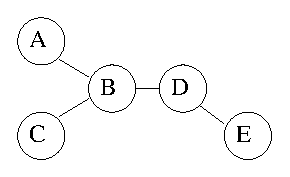
\includegraphics[width=0.4\columnwidth]{figures/mrf.eps}
    \caption{An example Markov random field with five random
    varaibles.}
    \label{fig:mrf}
%\end{wrapfigure}
\end{figure}


In an MRF, two variables $A$ and $B$ are
\textit{conditionally independent} from each other, if there
is at least one variable observed in each and every path
between $A$ and $B$.
That is, 
\[
p(A \mid \mX_{\text{obs}}, B) = p(A \mid \mX_{\text{obs}}),
\]
if there is no path between $A$ and $B$ without any observed
variable. $\mX_{\text{obs}}$ is the state of all observed
variables.

In this sense, we define the \textit{Markov blanket} of a
random variable as the set of all immediate neighboring
variables. If all the variables in the Markov blanket of another
variable were observed, the variable would be independent from all
other variables conditioned on the variables in the Markov
blanket.

In the example MRF in Fig.~\ref{fig:mrf}, there are five
random variables; $A$, $B$, $C$, $D$ and $E$. Let us
consider the variable $A$. When $D$ is observed, $A$ is
conditionally independent from $E$ since $D$ is the observed
in the only path $A$--$B$--$D$--$E$ between them. However,
$A$ and $C$ are mutually dependent, as the path
$A$--$B$--$C$ has no observed variable.

In this example, the Markov blanket of $D$ consists of $B$ and
$E$. Whenever both $B$ and $E$ are observed, $D$ is
conditionally independent from all other variables, in this
case $A$ and $C$, regardless of the connectivity in the
graph.

This conditional independence property provides a means to
parallelize a sampling procedure by Gibbs sampling. Let
us, for instance, assume that we run a Gibbs sampler to
collect samples from the example MRF in Fig.~\ref{fig:mrf}. One way is to grab a
sample from one variable at a time, sequentially. However,
if we consider the fact that $A$, $E$ and $C$ are
conditionally independent from each other when $B$ and $D$
are observed, we can use the following schedule for the
Gibbs sampler repeatedly:
\begin{enumerate}
    \itemsep 0em
    \item Sample from $p(A\mid B)$, $p(C \mid B)$ and $p(D
        \mid B, E)$ in parallel.
    \item Sample from $p(B \mid A, C, D)$ and $p(E \mid D)$
        in parallel.
\end{enumerate}
This will greatly speed up the sampling process, assuming
that parallel computation is easily accessible and
implementable.

Now it is easy to see why it is difficult to evaluate
statistics of a fully-connected Boltzmann machine by
collecting samples. When the Markov blanket of each unit
consists of all other units, sampling must be done for each
unit sequentially. This has led to attempts to overcome this
problem by imposing structural restrictions to a Boltzmann
machine using the property of conditional independence of an
MRF. Some of these attempts will be described in this section.

\subsection{Restricted Boltzmann Machines}
\label{sec:rbm}

A restricted Boltzmann machine (RBM) proposed by
\citet{Smolensky1986} is a variant of a Boltzmann machine
that has a bipartite structure such that each visible unit
is connected to all hidden units and each hidden unit to all
visible units, but there are no edges between the same type of units
(see Fig.~\ref{fig:rbm_dbm}(a) for illustration). In other
words, we put constraints in the energy of a Boltzmann
machine \eqref{eq:bm_energy} so that $\mU = \mzero$ and $\mV =
\mzero$.  Then, the energy is simplified into 
\begin{align}
    \label{eq:rbm_energy}
    -E(\vx, \vh \mid \TT) = \vb^\top \vx + \vc^\top \vh +
    \vx^\top \mW \vh.
\end{align}

\begin{figure}[t]
    \begin{minipage}{0.48\textwidth}
        \centering
        \psfrag{x_1}[Bc][Bc][1][0]{$x_1$}
        \psfrag{x_2}[Bc][Bc][1][0]{$x_2$}
        \psfrag{x_p}[Bc][Bc][1][0]{$x_p$}
        \psfrag{h_1}[Bc][Bc][1][0]{$h_1$}
        \psfrag{h_2}[Bc][Bc][1][0]{$h_2$}
        \psfrag{h_q}[Bc][Bc][1][0]{$h_q$}
        \psfrag{W}[Cc][Cc][1][0]{$\mW$}
        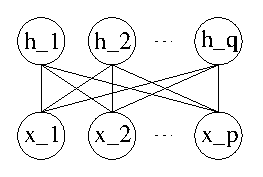
\includegraphics[width=0.65\columnwidth]{figures/rbm.eps}
    \end{minipage}
    \begin{minipage}{0.48\textwidth}
        \centering
    \psfrag{x_1}[Bc][Bc][1][0]{$x_1$}
    \psfrag{x_2}[Bc][Bc][1][0]{$x_2$}
    \psfrag{x_p}[Bc][Bc][1][0]{$x_p$}
    \psfrag{h_1}[Bc][Bc][1][0]{$h_1^{\qlay{1}}$}
    \psfrag{h_2}[Bc][Bc][1][0]{$h_2^{\qlay{1}}$}
    \psfrag{h_q}[Bc][Bc][1][0]{$h_{q_{\qlay{1}}}^{\qlay{1}}$}
    \psfrag{z_1}[Bc][Bc][1][0]{$h_1^{\qlay{L}}$}
    \psfrag{z_2}[Bc][Bc][1][0]{$h_2^{\qlay{L}}$}
    \psfrag{z_q}[Bc][Bc][1][0]{$h_{q_{\qlay{L}}}^{\qlay{L}}$}
        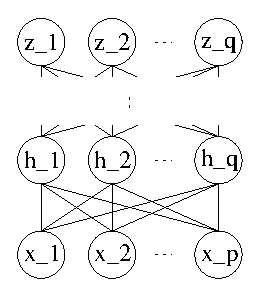
\includegraphics[width=0.65\columnwidth]{figures/dbm.eps}
    \end{minipage}

    \vspace{2mm}
    \begin{minipage}{0.48\textwidth}
        \centering
        \small
        (a) Restricted Boltzmann Machine
    \end{minipage}
    \begin{minipage}{0.48\textwidth}
        \centering
        \small
        (b) Deep Boltzmann Machine
    \end{minipage}
    \caption{Illustrations of restricted and deep Boltzmann machines.}
    \label{fig:rbm_dbm}
\end{figure}

Contrary to the fully-connected Boltzmann machine, the
Markov blanket of each unit consists only of the units of an
opposite type.  For instance, the Markov blanket of a
visible unit $x_i$ is the set of all hidden units, and that of
a hidden unit $h_j$ is the set of all visible units. Simply
put, the hidden units are conditionally independent given a
state of the visible units, and vice versa.

This conditional independence has two positive consequences
in computing the statistics required for learning the
parameters of an RBM.  Firstly, Gibbs sampling can be
implemented efficiently by parallelizing the sampling
procedure. The states of the units in each type of layer,
either a visible or hidden layer, can be sampled in parallel
given the state of the units in the other type of layer.
Essentially, samples are collected repeatedly from the
following distributions alternately:
\begin{align}
    \label{eq:rbm_cond_x}
    &p(\vx \mid \vh, \TT) = \prod_{i=1}^p \nu_i^{x_i} (1 -
    \nu_i^{1 - x_i}), \\
    \label{eq:rbm_cond_h}
    &p(\vh \mid \vx, \TT) = \prod_{j=1}^q \mu_j^{h_j} (1 -
    \mu_j^{1 - h_j}),
\end{align}
where
\begin{align*}
    \nu_i = p(x_i = 1 \mid \vh, \TT) = \phi\left( \sum_{j=1}^q
    w_{ij} h_j + b_i \right), \\
    \mu_j = p(h_j = 1 \mid \vx, \TT) = \phi\left( \sum_{i=1}^p
    w_{ij} x_i + c_j \right).
\end{align*}
Effectively, in just two parallelized steps, the state of
each unit is replaced by a new sample.  See
Fig.~\ref{fig:rbm_gibbs} for an illustration of Gibbs
sampling in the case of RBMs.

\begin{figure}[t]
    \centering
    \psfrag{x0}[Bc][Bc][0.95][0]{$\vx^{\qt{0}}$}
    \psfrag{h0_h_x0}[Bc][Bc][0.95][0]{$\vh^{\qt{0}}\sim \vh \mid \vx^{\qt{0}}$}
    \psfrag{x1_x_h0}[Bc][Bc][0.95][0]{$\vx^{\qt{1}}\sim \vx \mid \vh^{\qt{0}}$}
    \psfrag{h1_h_x1}[Bc][Bc][0.95][0]{$\vh^{\qt{1}}\sim \vh \mid \vx^{\qt{1}}$}
    \psfrag{x2_x_h1}[Bc][Bc][0.95][0]{$\vx^{\qt{2}}\sim \vx \mid \vh^{\qt{1}}$}
    \psfrag{h2_h_x2}[Bc][Bc][0.95][0]{$\vh^{\qt{2}}\sim \vh \mid \vx^{\qt{2}}$}
    \psfrag{x3_x_h2}[Bc][Bc][0.95][0]{$\vx^{\qt{3}}\sim \vx \mid \vh^{\qt{2}}$}
    \psfrag{h3_h_x3}[Bc][Bc][0.95][0]{$\vh^{\qt{3}}\sim \vh \mid \vx^{\qt{3}}$}
    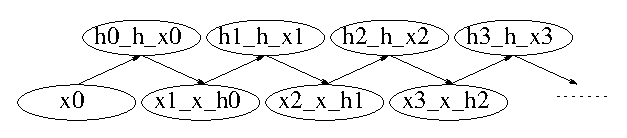
\includegraphics[width=0.95\columnwidth]{figures/bgibbs.eps}
    \caption{An illustration of performing a block Gibbs
    sampling on a restricted Boltzmann machine. $\vx_0$ is
    initialized to a random binary vector.}
    \label{fig:rbm_gibbs}
\end{figure}

Furthermore, it is easy to see that we can efficiently
compute the posterior distribution over the hidden units
exactly, since the posterior distribution is fully
factorized. The exact posterior distribution ${p(\vh \mid
\vx, \TT)}$ is given in Eq.~\eqref{eq:rbm_cond_h}. This
enables us to exactly compute the first term of the
gradient in Eq.~\eqref{eq:bm_grad}:
\begin{align}
    \label{eq:rbm_grad}
    \left< \frac{\partial
    \left(-E(\vx^{(n)}, \vh\mid\TT)\right)}{\partial \theta}
    \right>_{\td} = 
    \frac{1}{N} \sum_{n=1}^N \left( \frac{\partial
    -E(\vx^{(n)}, \vmu^{(n)} \mid \TT)}{\partial \theta}
    \right),
\end{align}
where $\vmu^{(n)} = \left[ \mu_1^{(n)}, \dots, \mu_q^{(n)}
\right]^\top$ and $\mu_j^{(n)} = p(h_j=1 \mid \vx^{(n)},
\TT)$. We used a shorthand notation $\td$ to denote the data
distribution which was replaced with the $N$
training samples $\left\{ \vx^{(1)}, \dots,
\vx^{(N)}\right\}$. 

However, this property of an RBM that enables parallelized
Gibbs sampling and exact computation of posterior
distribution over hidden units do \textit{not} fully avoid
the difficulty in computing the second term of the gradient.
Firstly, this efficient parallelized implementation does not
overcome the fundamental weakness of Gibbs sampling that it
is easy to get trapped in a single mode (see
Section~\ref{sec:gibbs}). Secondly, a sample gradient at
each time computed using samples from Gibbs sampling tends
to have high variance, which easily leads to unstable
learning.

In the remainder of this section, we describe an efficient
learning algorithm for an RBM based on the principle of
minimizing contrastive divergence, proposed by
\citet{Hinton2002}. 



\subsubsection{Product of Experts}
\label{sec:poe}

A product of experts (PoE\nomenclature{PoE}{Product of Experts}) \citep{Hinton2002} is a model that
combines multiple tractable probabilistic models, or
experts, by multiplying their contributions and
normalization
the product to sum up to one. The probability assigned to a
single input vector $\vx$ can then be written as
\begin{align}
    \label{eq:poe}
    p(\vx \mid \TT) = \frac{\prod_{j=1}^q \varphi_j(\vx \mid
    \TT_j)}{\sum_{\vx'} \prod_{j=1}^q \varphi_j(\vx' \mid
    \TT_j)},
\end{align}
where $\varphi_j$ is the positive contribution of the $j$-th
expert parameterized by $\TT_j$, and the denominator is the
normalization constant. It is not necessary for each
$\varphi_j$ to be a valid probability, since their product
will be normalized afterward.

By replacing $\varphi_j(\vx \mid \TT_j)$ with
$\tilde{\varphi_j}(\vx \mid
\TT_j)=\varphi_j(\vx\mid\TT_j)-1$, we may rewrite
Eq.~\eqref{eq:poe} as
\begin{align}
    \label{eq:poe2}
    p(\vx \mid \TT) = \frac{1}{Z(\TT)}\prod_{j=1}^q \left[ 1 +
    \tilde{\varphi}_j(\vx \mid
    \TT_j)\right],
\end{align}
where we used $Z(\TT)$ for the normalization constant. 

If we assume that there is a \textit{binary} hidden variable
associated with each expert, Eq.~\eqref{eq:poe2} can be
written as a marginal probability of the joint
probability of both the visible and hidden variables:
\begin{align}
    \label{eq:poe2_joint}
    p(\vx \mid \TT) = \sum_{\vh} p(\vx, \vh \mid \TT) =
    \sum_{\vh} \frac{1}{Z(\TT)} \prod_{j=1}^q
    \tilde{\varphi}_j (\vx \mid \TT_j)^{h_j}.
\end{align}
Furthermore, one can clearly see that the posterior
probability of $\vh$ given the state of $\vx$ is factorized
so that each $h_j$ is independent from all other hidden
variables. The posterior probability of $h_j$ is given by
\begin{align}
    \label{eq:poe_cond_h}
    p(h_j = 1 \mid \vx, \TT_j) = \frac{\tilde{\varphi}_j(\vx
    \mid \TT_j)}{1 + \tilde{\varphi}_j(\vx \mid \TT_j)}.
\end{align}

If it is further assumed that the choice of $\varphi_j$'s
makes the conditional probability of $\vx$ 
factorized, as was the case with RBMs, efficient 
parallelized Gibbs sampling can be implemented for the PoE.
One example of a contribution $\varphi_j$ or
$\tilde{\varphi}_j$, is 
\[
\tilde{\varphi}_j(\vx \mid \TT_j) = \exp\left\{ c_j +
\sum_{i=1}^p w_{ij} x_i \right\},
\]
which leads to the factorized conditional probability
\begin{align}
    \label{eq:poe_cond_x}
p(\vx \mid \vh, \TT) &= \frac{1}{Z(\TT)} \exp\left\{
\sum_{j=1}^q h_j c_j + \sum_{i=1}^p \sum_{j=1}^q w_{ij} x_i
h_j \right\} 
\nonumber \\
&= \frac{1}{Z'(\TT)} \prod_{i=1}^p \exp\left\{
\sum_{j=1}^q w_{ij} h_j
\right\}^{x_i},
\end{align}
where $Z'(\TT) = Z(\TT) \exp\left\{ \sum_j h_j c_j \right\}$
is a new normalization constant.

This model corresponds in fact exactly to the RBM
\citep{Freund1994}, under
certain constraints, such as (1) one of the experts is
always on to act as a visible bias in an RBM and (2) $\vx
\in \left\{ 0, 1 \right\}^p$. Comparing
Eqs.~\eqref{eq:poe_cond_h} and \eqref{eq:poe_cond_x} against
Eqs.~\eqref{eq:rbm_cond_h} and \eqref{eq:rbm_cond_x}, we see
that an RBM
is a special case of the PoE, and a learning algorithm for
PoEs can be immediately applied to an RBM.

Another example of PoE models that results in a factorized
conditional distribution is the exponential family harmonium
proposed by \citet{Welling2005}. The exponential family
harmonium assumes that the prior distributions of visible
variables
$\vx$ and hidden variables $\vh$ belong to the exponential
family. This implies that both conditional and posterior
distributions are in
the form of the exponential family distributions.

\subsubsection{Interpolation between Data and Model
Distributions and Contrastive Divergence}
\label{sec:contrastive_divergence}

Consider now a series of distributions that are
defined by running a Gibbs sampler for $k$ steps
under a PoE with a factorized conditional distribution for
visible variables. 

A distribution $P_0$ is defined to be the data distribution
$D$ from which a set of training samples was sampled. Since
the goal of the model is to model this distribution as well
as possible, the form of this distribution is assumed to be
unknown \textit{a priori}. 

Let $X_k = \left\{ \vx_k^{(1)}, \dots, \vx_k^{(N)} \right\}$
be a set of samples from $P_k$. We may then define a set of
samples $X_{k+1}$. First, we collect hidden samples $H_k =
\left\{ \vh_k^{(1)}, \dots, \vh_k^{(N)} \right\}$, where
each $\vh_k^{(n)}$ is a sample from the posterior
distribution $p(\vh \mid \vx = \vx_k^{(n)}, \TT)$.  Given
$H_k$, we collect samples or their respective means by the
conditional distribution such that $X_{k+1} = \left\{
\vx_{k+1}^{(1)}, \dots, \vx_{k+1}^{(N)}\right\}$, where
\[
\vx_{k+1}^{(n)} \sim \vx \left| \vh = \vh_k^{(n)}, \TT.
\right.
\]
We call the distribution, represented by the samples in
$X_{k+1}$, $P_{k+1}$.

Starting from the distribution $P_0$, $P_{k}$ in the limit
of $k \to \infty$ converges to the model distribution which
is the stationary distribution of the Markov Chain defined
by the Gibbs sampler used (see Section~\ref{sec:mcmc}). It
does not matter at all that we start the chain from the
training samples, rather than randomly chosen states,
assuming that the Gibbs chain is ergodic (see
Eq.~\eqref{eq:mcmc_ergodic} for its definition). 

%In
%Fig.~\ref{fig:gibbs_interpolation}, the interpolation from
%$P_0$ to $P_\infty$ by the Gibbs sampling is described.
%\tred{figure: Gibbs sampling in RBM: P0 -> P1 -> \dots ->
%P$\infty$}

Under these definitions, we may write the objective of
learning in RBMs, and respectively PoEs with a factorized
conditional distribution of visible variables, by $\KL(P_0
\| P_\infty)$. There $P_\infty$ is the model distribution
that can be described by the samples collected by running a
Gibbs sampler for a long time starting from the set of training
samples.

With these interpolated distributions, \citet{Hinton2002}
proposed a learning algorithm that minimizes a contrastive
divergence, instead of maximizing the log-likelihood. The
$k$-step contrastive divergence
(CD\nomenclature{CD}{Contrastive divergence}) is defined as a
difference between $\KL(P_0 \| P_{\infty})$ and $\KL(P_k \|
P_\infty)$. Minimizing it is equivalent to maximizing
the log-likelihood in the infinite limit of $k$, since
$\KL(P_\infty \| P_\infty) = 0$.

The gradient of the $k$-step CD is, then,
\begin{align}
    \label{eq:rbm_cd_grad}
    \frac{\partial \CD_k}{\partial \theta} \approx
    \left< \frac{\partial
    \left(-E(\vx^{(n)}, \vh\mid\TT)\right)}{\partial \theta}
    \right>_{P_0} 
    -
    \left< \frac{\partial
    \left(-E(\vx, \vh\mid\TT)\right)}{\partial \theta}
    \right>_{P_k},
\end{align}
where $\CD_k = \KL(P_0 \| P_{\infty}) - \KL(P_k
\| P_\infty)$. This approach is directly applicable to the
enhanced gradient described in
Section~\ref{sec:enhanced_grad} by replacing $\tf$ with
$P_k$ in Eqs.~\eqref{eq:enh_w}--\eqref{eq:enh_b}.

This method has a huge computational advantage over
maximizing the log-likelihood exactly in a naive way. As one
can immediately see, computing Eq.~\eqref{eq:rbm_cd_grad}
requires neither running the Gibbs sampler for indefinite
time nor checking the convergence of the sampling chain.
Empirically, minimizing CD was found to learn a good model
even with $k$ as small as $1$\footnote{ From here on, we
will occasionally refer to the learning algorithm that
minimizes CD as CD learning, when there is no ambiguity.  }.

Although minimizing CD has been used successfully in
practice since it was introduced,
\cite{Carreira-Perpinan2005,Bengio2009} showed that it is a
biased estimate of the true log-likelihood with a finite
$k$. This is contrary to the stochastic approximation
procedure described in Section~\ref{sec:sap}, which is
guaranteed to converge to the right maximum-likelihood
estimate under some mild assumptions. However, minimizing CD
is preferable in many cases,
%, usually where the aim of
%learning is not to find a good \textit{generative} model, 
as
much smaller learning rate needs to be used with the
stochastic approximation procedure, especially using a plain
Gibbs sampling (see, e.g., \citep{Hinton2012rbm}).

For detailed justification on minimizing CD, we refer any
interested reader to \citep{Bengio2009}.

\subsection{Deep Boltzmann Machines}
\label{sec:dbm}

The deep Boltzmann machine (DBM\nomenclature{DBM}{Deep Boltzmann
machine}) was proposed by
\citet{Salakhutdinov2009a} as a relaxed version of an RBM.  A
DBM simply stacks multiple additional layers of hidden units
on the layer of hidden units of an RBM. As was the case with
an RBM, consecutive layers are fully connected, while there
is no edge among the units in one layer. See
Fig.~\ref{fig:rbm_dbm}(b) for an example structure of a DBM.

The energy function is defined as
\begin{align}
    \label{eq:dbm_energy}
    -E(\vx, \vh \mid \TT) = \vb^\top \vx +
    \vc_{\qlay{1}}^\top \vh_{\qlay{1}}
    + \vx^\top \mW \vh_{\qlay{1}} + \sum_{l=2}^L \left(
    \vc_{\qlay{l}}^\top
    \vh_{\qlay{l}} + \vh_{\qlay{l-1}}^\top \mU_{\qlay{l-1}}
    \vh_{\qlay{l}} \right),
\end{align}
where $L$ is the number of hidden layers. The state and
biases of the hidden units at the $l$-th hidden layer and
the weight matrix between the $l$-th and $(l+1)$-th layers
are respectively defined by
\begin{align*}
    \vh_{\qlay{l}} = \left[ h_{1}^{\qlay{l}}, \dots,
    h_{q_l}^{\qlay{l}} \right]^\top,
    \vc_{\qlay{l}} = \left[ c_{1}^{\qlay{l}}, \dots,
    c_{q_l}^{\qlay{l}} \right]^\top, 
    \mU_{\qlay{l}} = \left[ u_{ij}^{\qlay{l}} \right],
\end{align*}
where $q_l$ is the number of the units in the $l$-th layer
and $\mU_{\qlay{l}} \in \RR^{q_l \times q_{l+1}}$.

Given a set $D$ of training samples, a DBM can also be
trained by maximizing the marginal log-likelihood in
Eq.~\eqref{eq:bm_mll}. However, unlike an RBM the posterior
distribution over the hidden units is not factorized, and
the variational approximation described in
Section~\ref{sec:bm_vari} needs to be used to compute the
statistics of the data distribution. 

The statistics of the model distribution can again be
estimated by using the Gibbs sampling. The layered structure
of a DBM makes it easy to parallelize the Gibbs sampling
procedure. Let us denote the state of the odd-numbered and
even-numbered hidden layers by $\vh_+$ and $\vh_-$,
respectively:
\[
\vh_+=\left[\vh_{\qlay{1}}^\top,
\vh_{\qlay{3}}^\top, \dots \right]^\top, 
    \vh_- = \left[
    \vh_{\qlay{2}}^\top, \vh_{\qlay{4}}^\top \dots \right]
\]
We can collect samples by repeating the following
steps:
\begin{enumerate}
    \itemsep 0em
    \item Sample $\vh_+$ in parallel, conditioned on $\vx$
        and $\vh_-$.
    \item Sample $\left\{ \vx, \vh_- \right\}$
        in parallel, conditioned on $\vh_+$.
\end{enumerate}

This procedure can similarly be used to estimate the
statistics of the data distribution by the variational
approximation. This is due to the fact that the fixed-point
update rules in Eq.~\eqref{eq:vari_update} of variational
parameters $\vmu^{\qlay{l}}$ in a single layer are mutually
independent given the variational parameters in the adjacent
layers. Based on this, we can perform the variational
fixed-point updates of the variational parameters of a DBM
efficiently using the following steps:
\begin{enumerate}
    \itemsep 0em
    \item Compute $\vmu_+$ in parallel using $\vx$ and $\vmu_-$
    \item Compute $\vmu_-$ in parallel using $\vmu_+$
\end{enumerate}
We used $\vmu_+$ and $\vmu_-$ to denote the variational
parameters of the odd-numbered and even-numbered hidden
layers, respectively.

It has been noticed by many researchers, for instance
\citet{Salakhutdinov2009a} and \citet{Desjardins2012} as
well as the author in \citepub{Cho2013ijcnn} and
\citepub{Cho2013icann}, that training
a DBM starting from randomly initialized parameters is not
trivial. 

In order to alleviate this difficulty,
\citet{Salakhutdinov2009a,Salakhutdinov2012} proposed an
algorithm that initializes the parameters of a DBM by
pretraining each layer separately starting from the bottom
layer. In \citepub{Cho2013icann}, yet another pretraining
algorithm was proposed that utilizes a deep autoencoder to
obtain a set of variational parameters for the hidden units
in the even-numbered hidden layers.  We will discuss those
pretraining algorithms later in Section~\ref{sec:dbm_pre}.

There have been other approaches to avoid this difficulty.
\citet{Montavon2012} suggested that a shifting
transformation that centers each unit, described briefly in
Section~\ref{sec:enhanced_grad}, helps training a
DBM directly from a set of randomly initialized parameters
at least when the size of the DBM is relatively small.  On
top of the shifting transformation, \citet{Desjardins2013}
proposed a metric-free natural gradient method that utilizes
the idea of natural gradient together with the subsampled
Hessian algorithm. 



\section{Boltzmann Machines and Autoencoders}
\label{sec:bm_aenc}

In this section, we try to describe the connections between
the Boltzmann machines and the autoencoders which we have
discussed earlier in Section~\ref{sec:linear_autoencoder}
and Section~\ref{sec:autoencoders}.

We begin by relating an RBM with an autoencoder that has
only a single hidden layer. This can be done by considering
the correspondence between the learning algorithms for the
two models. We will discuss this from the perspectives of contrastive
divergence learning and score matching
\citep{Hyvarinen2005}. These connections were respectively
discovered and presented by \citet{Bengio2009},
\citet{Swersky2011} and \citet{Vincent2011}.

We continue on to describing a deep belief network
\citep{Hinton2006nc} which is an extension of the sigmoid
belief network described earlier in
Section~\ref{sec:sbn_dbn} as one of the related approaches
of deep autoencoders. 
%Furthermore, in doing so, we introduce
%a concept of layer-wise pretraining which constitutes an
%important part of learning algorithms of deep neural
%networks.

\subsection{Restricted Boltzmann Machines and Autoencoders}
\label{sec:rbm_aenc}

Let us start with rather shallow models that have only a
single hidden layer consisting of nonlinear units, which are
restricted Boltzmann machines and autoencoders with a single
intermediate hidden layer. 

We briefly discuss two different ways to relate RBMs to
shallow autoencoders here. However, it should be noticed
that these are \textit{not} the only ways \citep[see,
e.g.,][for another interpretation that unifies RBMs and
autoencoders]{Ranzato2007a}.

\subsubsection{Contrastive Divergence and Reconstruction Error}
\label{sec:cd_rerr}

In \citep{Bengio2009}, learning parameters of an RBM by
minimizing contrastive divergence was justified by
considering an expansion of the gradient of the marginal
log-likelihood of an RBM in Eq.~\eqref{eq:rbm_grad}. 

As we defined the interpolated distributions between the
data and model distributions in
Section~\ref{sec:contrastive_divergence}, let us here
consider a potentially infinite sequence \\
$\left\{
\left(\vx^{\qt{0}}, \vh^{\qt{0}}\right),
\left(\vx^{\qt{1}},
\vh^{\qt{1}}\right), \dots \right\}$, where
\[
\vx^{\qt{n}} \sim \vx \mid \vh^{\qt{n-1}}, \TT
\]
and
\[
\vh^{\qt{n}} \sim \vh \mid \vx^{\qt{n}}, \TT.
\]
$\vx^{\qt{0}}$ denotes a training sample.

In this case, \citet{Bengio2009} showed that the gradient of
the marginal log-likelihood, considering only a single
sample for now, can be expanded by
\begin{align}
    \label{eq:rbm_grad_exp}
    \frac{\partial \LL(\TT)}{\partial \theta} &= 
    \sum_{s=1}^{t-1} \left( \E\left[ \frac{\partial \log
    p(\vx^{\qt{s}} \mid \vh^{\qt{s}})}{\partial \theta}
    \right]  + \E \left[ \frac{\partial \log p(\vh^{\qt{s}}
    \mid \vx^{\qt{s+1}} )}{\partial \theta} \right]
    \right) 
    \nonumber \\
    &\phantom{\sum_{s=1}^{t-1}} + \E \left[ \frac{\partial \log
    p(\vx^{\qt{t}})}{\partial \theta} 
    \right],
\end{align}
where the terms inside the summation and the last term
converge to zero as $t$ grows. The expectations are computed
over the data distribution. Dependency on $\TT$ is omitted
to make the expression less cluttered.

When only the first two terms of the expansion in
Eq.~\eqref{eq:rbm_grad_exp} are considered, we get the
update direction that minimizes the contrastive divergence
with $k=1$.
The remaining terms determine the bias in the resulting
model.

\citet{Bengio2009} went one more step to investigate the
case of truncating even earlier. In that case, the truncated
expression becomes
\[
\sum_{\vh} p(\vh \mid \vx^{\qt{0}}) \frac{\partial \log
p(\vx^{\qt{1}} \mid \vh)}{\partial \theta}.
\]
If we use a mean-field approximation to replace
each component $h_j$ of $\vh$ inside $\log
p(\vx^{\qt{1}} \mid \vh)$ with its posterior mean $\hat{h}_j =
\E\left[ h_j \mid \vx^{\qt{0}} \right]$, we get
\begin{align}
    \label{eq:rbm_grad_exp_ext}
    \frac{\partial \log p(\vx^{\qt{1}} \mid \hat{\vh})}{\partial \theta}.
\end{align}
Let us rewrite it by adopting our usual notation using
Eq.~\eqref{eq:unsup_train} such that we assume to be given
a set of training samples as
\[
D=\left\{ \vx^{(n)} \right\}_{n=1}^N.
\]
Eq.~\eqref{eq:rbm_grad_exp_ext} becomes
\[
\sum_{n=1}^N \frac{\partial \log p(\vx^{(n)} \mid
\hat{\vh}^{(n)})}{\partial \theta}.
\]
It is straightforward to see that this is the gradient of
the cross-entropy loss of a single-layer autoencoder with a
single hidden layer of sigmoid hidden units.

This result says that minimizing contrastive divergence is
an extreme \textit{stochastic approximation} of maximizing
the marginal log-likelihood, while minimizing the
reconstruction error or cross-entropy corresponds to a
\textit{deterministic approximation}. Since the latter
truncated one more term from the expansion, the latter
obviously results in a more biased estimation, if we look at
the resulting model as an RBM. 

However, the objective function of an autoencoder, which is
a negative reconstruction error, can be exactly and
efficiently computed, while computing the marginal
log-likelihood of an RBM is intractable. This makes it
easier to learn parameters by minimizing the reconstruction
error compared to either minimizing the contrastive
divergence or maximizing the marginal log-likelihood
directly.

\subsubsection{Gaussian Restricted Boltzmann Machines, Score
Matching and Autoencoders}
\label{sec:grbm}

Let us define an RBM that can handle continuous visible
units by replacing binary visible units with Gaussian units.
The energy function of this RBM, called a Gaussian-Bernoulli
RBM \citep[GRBM,][]{Hinton2006} is then,
\begin{align}
    \label{eq:grbm_energy}
    -E(\vx, \vh \mid \TT) = -\sum_{i=1}^p \frac{(x_i -
    b_i)^2}{2\sigma_i^2} + \sum_{j=1}^q h_j c_j +
    \sum_{i=1}^p \sum_{j=1}^q \frac{x_i}{\sigma_i^2} h_j
    w_{ij}.
\end{align}
The conditional distributions of the visible and hidden
units are defined by
\begin{align}
    \label{grbm:conditional_visible}
    p(x_i = x | \vh) &= \N \left(x \:\Bigl|\: b_i + 
    \sum_j h_j W_{ij} \:,\: \sigma_i^2 \right)
\end{align}
and
\begin{align}
    \label{grbm:conditional_hidden}
    p(h_j = 1 | \vx) &= \phi \left( c_j +  \sum_i W_{ij}
    \frac{x_i}{\sigma_i^2} \right),
\end{align}
where $\phi$ is again a sigmoid function.

In other words, each visible unit conditionally follows a
Gaussian distribution whose mean is determined by the
weighted sum of the states of the hidden units. The
conditional probability of each hidden unit being one is
determined by the weighted sum of the states of the visible
units \textit{scaled} by their variances\footnote{
The energy function of a GRBM was originally proposed by
\citet{Hinton2006} to be
\[
    -E(\vx, \vh \mid \TT) = -\sum_{i=1}^p \frac{(x_i -
    b_i)^2}{2\sigma_i^2} + \sum_{j=1}^q h_j c_j +
    \sum_{i=1}^p \sum_{j=1}^q \frac{x_i}{\sigma_i} h_j
    w_{ij},
\]
which results in a conditional probability of a visible unit 
\[
p(x_i = v | \vh) = \N \left(x \:\Bigl|\: b_i + 
\sigma_i \sum_j h_j W_{ij} \:,\: \sigma_i^2 \right).
\]
In order to avoid the standard deviation $\sigma_i$
affecting the mean, it was proposed in
\citepub{Cho2011icann} that the energy function be modified
so that $\sigma_i$ does not influence the conditional mean
of the visible unit.  In \citepub{Cho2011icann}, it was
claimed that this formulation makes estimating $\sigma_i$'s
easier, and hence we use the modified definition of the energy
function here.
}.
It should be noticed that despite the change of the visible
units' types, there is essentially no change in its learning
algorithm compared to the original RBM with binary visible
units.

In this case, an alternative learning algorithm called
\textit{score matching} proposed by \citet{Hyvarinen2005},
can be used instead of the stochastic approximation
procedure or CD learning. Score matching can be used to
estimate the parameters of a model whose
\textit{differentiable} unnormalized probability can be
tractably computed exactly, while computing its
normalization constant is intractable. This requirement
reminds us of a PoE described earlier in
Section~\ref{sec:poe} which is a family of models that
includes a GRBM.

We start by writing a GRBM in the form of PoE:
\begin{align}
    \label{eq:grbm_poe}
    \log p(\vx \mid \TT) &= -\frac{(b_i - x_i)^2}{2\sigma_i^2}
    + \sum_{j=1}^q \log \left( 1 + \exp\left\{ \sum_{i=1}^p
    \frac{x_i}{\sigma_i^2} w_{ij} + c_j \right\}\right) -
    \log Z(\TT) 
    \nonumber \\
    &= \log p^*(\vx \mid \TT)  - \log Z(\TT).
\end{align}
Then, the score function of the GRBM is
\begin{align}
    \label{eq:grbm_score}
    \psi_i (\vx \mid \TT) &= \frac{\partial \log p^*(\vx \mid
    \TT)}{\partial x_i} 
    \nonumber \\
    &= \frac{b_i - x_i}{\sigma_i^2} + \sum_{j=1}^q \hat{h}_j
    \frac{w_{ij}}{\sigma_i^2}.
\end{align}
Furthermore, we will need
\begin{align*}
    %\label{eq:grbm_score_grad}
    \frac{\partial \psi_i(\vx \mid \TT)}{\partial x_i} =
    -\frac{1}{\sigma_i^2} + \sum_{j=1}^q \hat{h}_j (1 -
    \hat{h}_j) \frac{w_{ij}^2}{\sigma_i^4},
\end{align*}
where $\hat{h}_j = \phi\left( \sum_{i=1}^p
\frac{x_i}{\sigma_i^2} w_{ij} + c_j \right)$ is the
activation probability of the $j$-th hidden units.

Given a set $D$ of $N$ training samples, score matching
then tries to minimize the following cost function
instead of maximizing the marginal log-likelihood:
\begin{align}
    \label{eq:grbm_sm_cost_orig}
    J(\TT) &= \frac{1}{N} \sum_{n=1}^N \sum_{i=1}^p \left[
    \frac{\partial \psi_i(\vx^{(n)} \mid \TT)}{\partial x_i}
    + \frac{1}{2} \psi_i (\vx \mid \TT)^2
    \right]
\end{align}

If we assume that the bias $b_i$ and the conditional
variance $\sigma_i$ to each visible unit are respectively
fixed to $0$ and $1$\footnote{ Fixing $b_i$ to $0$ can be
indirectly achieved by normalizing each component of
training samples to have a zero-mean, and it has been a
usual practice to ignore $\sigma_i$ by forcing it to $1$
\citep[see, e.g.,][]{Hinton2012rbm}.  }, the cost function in
Eq.~\eqref{eq:grbm_sm_cost_orig} can be rewritten as
\begin{align*}
    J(\TT) = \frac{1}{N} \sum_{n=1}^N \left[ \frac{1}{2}
    \sum_{i=1}^p \left( \sum_{j=1}^q \hat{h}_j w_{ij} - x_i
    \right)^2 + \sum_{i=1}^p \sum_{j=1}^q h_j(1 - h_j)
    w_{ij}^2 \right] + C,
\end{align*}
where $C$ is a constant that does not depend on $\TT$.

It is easy to see that the first term inside the summation
is the reconstruction error of a single-layer autoencoder
with a tied set of weights $\mW$ (see
Eq.~\eqref{eq:autoencoder_cost}). The other term can be
considered as a regularization term.

Hence, this leads us to understand that learning the
parameters of a GRBM by score matching is equivalent to
learning the parameters of a single-layer autoencoder that
has a hidden layer having nonlinear sigmoidal units by
minimizing the reconstruction error with a regularization
\citep{Swersky2011}. Furthermore, this connection gives a
justification on using a tied set of weights for the
encoder and decoder of an autoencoder \citep{Vincent2011}.

Additionally to an ordinary autoencoder, \citet{Vincent2011}
showed a connection between a denoising autoencoder (see
Section~\ref{sec:dae}) and a modified form of GRBM, again
via score matching. 


\clearpage
\subsection{Deep Belief Network}
\label{sec:dbn}

%\begin{figure}[t]
\begin{wrapfigure}{I}{0.4\textwidth}
    \centering
    \psfrag{x_1}[Bc][Bc][1][0]{$x_1$}
    \psfrag{x_2}[Bc][Bc][1][0]{$x_2$}
    \psfrag{x_p}[Bc][Bc][1][0]{$x_p$}
    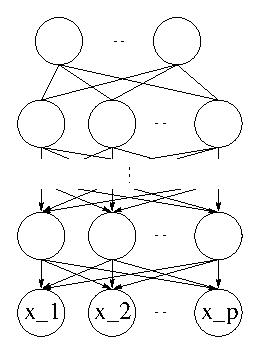
\includegraphics[width=0.27\columnwidth]{figures/dbn.eps}
    \caption{An illustration of a deep belief network. Note
    that the top two layers are connected to each other by
    \textit{undirected} edges.}
    \label{fig:dbn}
    \vspace{-2mm}
\end{wrapfigure}
%\end{figure}

In Section~\ref{sec:sbn_dbn}, we presented the sigmoid
belief network in relation with a deep autoencoder and
subsequently briefly described the deep belief network.
Here, we present another view of the DBN as a combination of
a sigmoid belief network and an RBM.

The deep belief network (DBN), proposed by
\citet{Hinton2006nc}, is a hybrid model that has both
directed and undirected edges.  The top two hidden layers
$\vh^{(L-1)}$ and $\vh^{(L)}$ are connected to each other 
(without any intra-layer edges) by undirected edges,
while all subsequent pairs of layers below are connected
with the directed downward edges. Hence, one might say that
the top two layers generatively model the \textit{prior}
distribution of $\vh^{(L-1)}$, and all the other hidden layers
below model the conditional distribution that generates the
states of the units in the layer immediately below. See
Fig.~\ref{fig:dbn} for the illustration.

In this case, as we did with Boltzmann machines previously,
we may define the energy as
\begin{align}
    \label{eq:dbn_energy}
    -E(\vx, \vh^{\qlay{1}}, \dots, \vh^{\qlay{L}} \mid \TT)
    = 
%    \nonumber
%    \\
    &\log p(\vx \mid \vh^{\qlay{1}}, \TT) + \sum_{l=1}^{L-2} \log
    p(\vh^{\qlay{l}} \mid \vh^{\qlay{l+1}}, \TT) 
    \nonumber \\
    &\phantom{= \log}+\log p(\vh^{\qlay{L-1}}, \vh^{\qlay{L}}, \TT) 
\end{align}
where the last term denotes the top two layers connected by
the undirected edges. The conditional distribution between
the consecutive intermediate hidden layers as well as between
the visible and first hidden layers is defined by
Eqs.~\eqref{eq:sbn_gen_h}~and~\eqref{eq:sbn_gen_x},
respectively.

Again, similarly to the Boltzmann machine, we can define the
joint probability of all units using a Boltzmann
distribution:
\begin{align*}
    p(\vx, \vh \mid \TT) = \frac{1}{Z(\TT)} \exp \left\{
    -E(\vx, \vh \mid \TT)
    \right\},
\end{align*}
where we simply used $\vh$ to denote the units in all hidden
layers.

A DBN maintains two sets of parameters as well as the
parameters for the top two layers.  The first two sets
$\TT_-$ and $\TT_+$ correspond to the recognition and
generation parameters of a sigmoid belief network.
Additionally, there is a separate set of parameters for the
parameters of a top-level RBM.

Using this hybrid architecture \citet{Hinton2006nc} proposed
an efficient learning algorithm that consists of two stages.
In the first stage, each pair of layers, starting from the
bottom, is \textit{pretrain}ed as if it were an RBM.

Specifically, the first pair of layers $\vx$ and
$\vh^{\qlay{1}}$
is trained as an RBM to model a given set of training
samples $D=\left\{ \vx^{(1)}, \dots, \vx^{(N)} \right\}$.
Once the training is over, we can efficiently and exactly
compute the posterior distribution over $\vh^{(1)}$ given
each training sample $Q(\vh^{\qlay{1}} \mid \vx^{(n)})$ and
collect samples from these distributions. We call the
distribution from which those samples were collected an
\textit{aggregate posterior} distribution
\[
\tilde{Q}\left( \vh^{\qlay{1}} \right) = \frac{1}{N}
\sum_{n=1}^N Q\left(\vh^{\qlay{1}} \mid \vx^{(n)}\right)
\]
Let us denote the set of the samples from this distribution by $D_1$. 

Then, the next pair of layers $\vh^{\qlay{1}}$ and
$\vh^{\qlay{2}}$ are pretrained to model $\tilde{Q}\left(
\vh^{\qlay{1}} \right)$ using the set $D_1$. From this RBM
we can again collect a set of samples $D_2$ from the next
aggregate posterior distribution $\tilde{Q}\left(
\vh^{\qlay{2}} \right)$. We continue this process up until
we pretrain the last pair of layers $\vh^{\qlay{L-1}}$ and
$\vh^{\qlay{L}}$. Let us use $\TT_0^{\qlay{l}}$ to indicate the
parameters of an RBM consisting of the $l$-th and $(l+1)$-th
layers, learned during the first stage.

The first stage corresponds to a layer-wise pretraining.
Instead of jointly optimizing all the layers at once, during
the first stage each pair of two consecutive layers is
optimized one by one starting from the bottom pair
consisting of the visible and first hidden layers. This
approach of adding more hidden layers in a DBN has been
shown to guarantee to improve the variational lower-bound of
the model \citep{Hinton2006nc}, and will be discussed more
in Section~\ref{sec:dbn_rbm}.

The second stage highly resembles the wake-sleep algorithm
used to estimate the parameters of a sigmoid belief network
from Section~\ref{sec:sbn_dbn}. The learning algorithm,
called the up-down algorithm, starts by initializing the
weights to those estimated during the first stage. The
recognition and generation parameters will be identical,
since the RBMs trained in the first stage use a tied set of
weights for both inference and generation. The parameters
between the top two layers will be $\TT_0^{\qlay{L-1}}$.

The \textit{up}-pass of the up-down algorithm corresponds to
the \textit{wake}-stage, and given a training sample, the
samples are collected from the approximate posterior
distributions over the hidden units using the recognition
weights up until the penultimate layer. The generation
parameters of the intermediate hidden layers are updated
using Eq.~\eqref{eq:sbn_wake}, while the parameters of the
top two layers are updated using the learning rule of an RBM
in Eq.~\eqref{eq:rbm_grad}.

At the \textit{down}-pass, unlike the \textit{sleep}-stage,
one does not attempt to collect model samples starting from
scratch. Rather, Gibbs sampling is run starting from the
samples of the penultimate layer collected during the
up-pass for several iterations, which reminds us of
minimizing contrastive divergence (see
Section~\ref{sec:contrastive_divergence}). From the samples
gathered by the several-step Gibbs sampling, the generation
parameters are used to generate samples of the subsequent
intermediate layers down until the visible layer. The
recognition parameters are then updated using
Eq.~\eqref{eq:sbn_sleep}. Unlike in the up-pass, the
parameters of the top two layers are \textit{not} adjusted
in the down-pass.

This model can thus be thought as combining a deep
autoencoder having stochastic hidden units together with a
top-level RBM. The stochastic deep autoencoder models both
the conditional distribution of a layer given the state of
the upper layer and the approximate posterior distribution
of a layer given the state of the lower layer. The prior
distribution of the penultimate hidden layer is learned by
the top-level RBM.

\subsubsection{Deep Energy Model}

Before ending this section, we will briefly introduce a deep
energy model (DEM\nomenclature{DEM}{Deep energy model})
proposed by \citet{Ngiam2011} as an alternative formulation
of combining a deep autoencoder with an RBM. A DEM extends
an RBM by introducing a nonlinear encoder with multiple
layers of \textit{deterministic} hidden units. According to
\citet{Ngiam2011}, this potentially avoids the difficulty
introduced by having stochastic hidden units in a deep
belief network.

Let us consider a GRBM from Section~\ref{sec:grbm}, however,
assuming that $\sigma_i=1$ for all $i=1,\dots,p$. The energy
function of a DEM is a modified form of
Eq.~\eqref{eq:grbm_energy} such that
\begin{align*}
    \label{eq:dem_energy}
    -E(\vx, \vh \mid \TT) = \sum_{i=1}^p x_i b_i
    + \sum_{j=1}^q h_j c_j +
    \sum_{i=1}^{p'} \sum_{j=1}^q f_i(\vx\mid \TT_f) h_j
    w_{ij},
\end{align*}
where $f_i(\vx \mid \TT_f)$ is the $i$-th component of an
output of a nonlinear encoder $f:\RR^p \to \RR^{p'}$
parameterized by $\TT_f$.

The parameters of both an RBM and an encoder can be
estimated by maximizing the marginal log-likelihood as usual
with an RBM. \citet{Ngiam2011} used the stochastic
approximation procedure with hybrid Monte Carlo
\citep{Neal1993} to estimate the statistics of the model
distribution.


\chapter{Unsupervised Neural Networks as the First Step}
\label{chap:pretraining}

So far in this thesis, we have considered unsupervised
and supervised neural networks separately.  In fact, our
main focus was on the unsupervised neural networks rather
than the supervised ones. We mostly discussed
autoencoders and Boltzmann machines, both of which aim to
learn the distribution of training samples and are not
specifically engineered for other tasks.

In Section~\ref{sec:bp_imp}, we briefly discussed the so
called layer-wise pretraining, where shallow
unsupervised neural networks were used to initialize the
parameters of a deep multi-layer perceptron (MLP). Notably,
a stack of, for instance, restricted Boltzmann machines used
for initializing an MLP was trained without any prior
knowledge that it will be used for classification.

This suggests that it may be possible or even beneficial
to utilize unsupervised neural networks as the first step to
train a more sophisticated model that aims to perform a
potentially different target task. For instance, an
unsupervised neural network such as a denoising autoencoder
or contractive autoencoder may be used to transform the
coordinate system of input samples into one that is more
useful for supervised learning tasks. A restricted Boltzmann machine
may be trained to facilitate training more sophisticated
deep Boltzmann machines, or it can learn the joint
distribution of inputs and outputs and use it to compute the
conditional distribution of an output given a new input.

In this chapter, we discuss some of the approaches proposed
recently to incorporate the power of generative modeling
provided by unsupervised neural networks to improve the
performance of another, often more complex neural network.  


\section{Incremental Transformation: Layer-Wise Pretraining}
\label{sec:layer_wise_pretraining}

Let us consider a classification task. We already
discussed earlier in Sections~\ref{sec:perceptron} and
\ref{sec:log_reg} that a simple perceptron without any
intermediate nonlinear hidden layer can perform this task
perfectly only if training samples are \textit{linearly
separable}. Otherwise, this simple neural network will fail to
do so.  However, even
if the training set has a nonlinear separating hyperplane,
an MLP which is essentially a perceptron with one or more
intermediate nonlinear hidden layers can be trained to
classify the samples, assuming that the MLP is large enough.

The feedforward computation starting from the bottom,
visible layer fixed to an input $\vx$ gradually performs
nonlinear transformations up until the last hidden layer.
Let $\vh=f(\vx)$ be the nonlinearly transformed
representation of $\vx$ by the feedforward pass of an MLP.
Then, the last part of the MLP essentially does a
perceptron-like \textit{linear} classification on $\vh$.

In other words, the encoder $f$ computed by the MLP attempts to
transform each sample $\vx^{(n)}$ into a new point
$\vh^{(n)}$ in a new coordinate system such that the set of
these new points $\tilde{D} = \left\{ (\vh^{(n)}, y^{(n)})
\right\}_{n=1}^N$ is as linearly separable as possible. It
does not matter whether the original training set $D=\left\{
(\vx^{(n)},y^{(n)}) \right\}_{n=1}^N$ is linearly
separable or not.

This process $f$ is carried out in an incremental fashion.
Each subsequent intermediate layer transforms the coordinate
system from the immediate lower layer such that the samples
become linearly separable after going through the multiple
layers of nonlinear transformations.
%
%the samples
%become more linearly separable.

%more evenly
%distributed and hence hopefully linearly separable, or
%better suited for other machine learning models. 

\begin{figure}[t]
    \centering
    \psfrag{x}[Bc][Bc][1][0]{$\vx$}
    \psfrag{h1}[Bc][Bc][1][0]{$\vh^{\qlay{1}}$}
    \psfrag{h2}[Bc][Bc][1][0]{$\vh^{\qlay{2}}$}
    \psfrag{y}[Bc][Bc][1][0]{$\vy$}
    \psfrag{(1)}[Bc][Bc][1.0][0]{Pretraining
    (1$^\text{st}$ layer)}
    \psfrag{(2)}[Bc][Bc][1.0][0]{Pretraining
    (2$^\text{nd}$ layer)}
    \psfrag{(3) Combine}[Bc][Bc][1.0][0]{}
    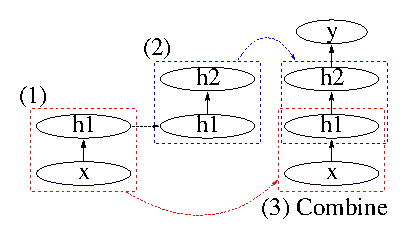
\includegraphics[width=0.7\columnwidth]{figures/pretrain_mlp.eps}
    \caption{Illustration of the layer-wise pretraining of
    a multi-layer perceptron. The dashed directed lines
    indicate \textit{copying} of either pretrained models or
    the activations of the hidden units of the pretrained
    models.}
    \label{fig:incr_feat}
\end{figure}

This suggests a possibility of incrementally building a
sequence of intermediate layers that gradually extract
better and better representations of data\footnote{We say
the \textit{representation is better} when better
\textit{generalization} performance on another machine
learning task, for instance classification, can be achieved
using the representation compared to using the raw
representation \citep{Bengio2007nips}.}. This is different
from
how the parameters of an MLP were estimated. For an MLP, we
first fix the structure of the model and jointly optimize
all layers, while what is being suggested here is different. We start with one visible and one hidden
layer to learn a \textit{transformation} that extracts a
somewhat better representation. Repeatedly, using the
representation from the previous stage, we train another
model with one visible and one hidden layer to learn a
still somewhat
better representation. See Fig.~\ref{fig:incr_feat}
for the illustration.

In fact, this approach of incrementally learning multiple
layers of representations constitutes one of the most important
principles in the field called \textit{deep learning}
\citep[see, e.g.,][]{Bengio2009a}.

\subsection{Basic Building Blocks: Autoencoder and Boltzmann
Machines}
\label{sec:basic_blocks1}

The most straightforward way to implement this incremental
feature learning is to consider each consecutive pair of
layers of an MLP separately. 

Each pair consists of a lower layer of visible units $\vx
\in \RR^p$ and an upper layer of nonlinear hidden units $\vh
\in \RR^q$, and they are connected by directed edges from
the lower to upper layers. A hidden activation, or hidden
state, is computed by 
\[
\vh = \phi\left( \mW^\top \vx + \vc \right),
\]
where $\phi$ is a component-wise nonlinearity.  This reminds
us of an encoder of an autoencoder (see
Eq.~\eqref{eq:ae_encoder}) or the conditional probability of
hidden units of a restricted Boltzmann machine (RBM, see
Eq.~\eqref{eq:rbm_cond_h}).

Hence, it is natural to estimate the parameters $\mW$ and
$\vc$ as if a pair of those two layers would form either an
autoencoder with a single hidden layer or a restricted
Boltzmann machine. We start from the bottom by training the
visible layer and the first hidden layer as if they formed
an RBM. Once the RBM is trained, we compute the posterior
distribution of hidden units and consider them as a new set
of training samples for an upper pair of layers consisting
of the first and second hidden layers. We repeat this step
until the last two hidden layers were trained as yet
another RBM. This same procedure can be done using
either ordinary or regularized autoencoder instead of the
RBMs.

An ordinary autoencoder \citep[see, e.g.,][and
Section~\ref{sec:autoencoders}]{Bengio2007nips}, a
regularized autoencoder \citep[see, e.g.,][and
Section~\ref{sec:spaenc}]{Ranzato2008} as
well as sparse coding \citep[see, e.g.,][and
Section~\ref{sec:sparse_coding}]{Raina2007} and a restricted
Boltzmann machine \citep[see, e.g.,][and
Section~\ref{sec:rbm}]{Hinton2006} as well as a sparse
restricted Boltzmann machine \citep[see, e.g.,][]{Lee2007}
have been used widely in this way to perform incremental
feature learning. The denoising autoencoder
\citep{Vincent2010} and contractive autoencoder
\citep{Rifai2011} discussed in Section~\ref{sec:dae_cae}
have recently been shown to be effective in this approach.

Once the sequence of these models is obtained it is
possible, though not necessary, to \textit{finetune} them
all together for a specific target task. For instance, an
MLP can be initialized by stacking the learned sequence and
be trained continuing from the \textit{pretrained}
parameters using backpropagation (see
Section~\ref{sec:backprop}). A deep autoencoder with more
than one intermediate layer can also benefit from this
approach \citep{Hinton2006}. In this context, the approach
of incremental feature learning is often referred to as a
\textit{layer-wise pretraining}. This layer-wise pretraining
has been successfully used to train a deep neural network
that has been known to be difficult to train well
starting from randomly initialized parameters.

\section{Unsupervised Neural Networks for Discriminative
Task}
\label{sec:dunn}

Throughout this thesis, we have mostly concentrated on
\textit{unsupervised} neural networks.  There are obvious
tasks to which these unsupervised neural networks can
trivially be applied.

For instance, \citet{Burger2012}, \citet{Xie2012} and
\citet{Cho2013} (\citepub{Cho2013icannA}) 
recently showed
that (denoising) autoencoder and restricted/deep Boltzmann
machines can denoise large, corrupted images.  The
performance of these neural networks was shown to be
comparable to, or sometimes better than, conventional
methods of image denoising such as BM3D \citep{Dabov2007} or
K-SVD \citep{Portilla2003}.  

A deep autoencoder initialized by a deep belief network
was shown to excel at extracting low-dimensional binary
codes for documents \citep{Salakhutdinov2009s}.  Also,
\citet{Salakhutdinov2007} showed that an RBM can be
successfully used for collaborative filtering. 

However, obviously, these unsupervised models cannot be used
directly for performing any supervised task.  This is
clear as none of these models have at their disposal known
outputs of training samples.

As in the layer-wise pretraining discussed earlier in this
chapter, however, the unsupervised neural networks can be
used to improve the discriminative performance of 
supervised models. In the layer-wise pretraining,
recursively stacking shallow unsupervised neural networks
was shown to extract better representations that are more
suitable for classification, which may be improved further by
finetuning the stack with backpropagation.

In the remainder of this section, we introduce other approaches
than the previously discussed layer-wise pretraining
that aim to improve the discriminative performance by
using unsupervised neural networks. These approaches
may use a separate unsupervised neural network, or combine a
supervised and an unsupervised neural network.

\subsection{Discriminative RBM and DBN}
\label{sec:drbm}

The most straightforward way to perform discriminative tasks
with an unsupervised neural network is to model the joint
probability distribution of both the input and output
$p(\vx, y)$. Once the network is trained, one can utilize
the joint distribution to perform a prediction on a new
sample $\vx$. 

Regardless of whether the task is classification or
regression, the best output $\hat{y}$ given a new sample
$\vx^*$ can be found by, for instance, the maximum a
posteriori (MAP):
\begin{align}
    \label{eq:gen_class}
    \hat{y} = \argmax_{y} p^*(\vx^*, y),
\end{align}
where we have used the unnormalized probability $p^*$ to
emphasize that there is no need to compute the potentially
intractable normalization constant. 

Alternatively, one may be interested in computing the
expected value of the output 
\begin{align}
    \label{eq:gen_class}
    \hat{y} = \frac{1}{Z} \sum_{y \in \mY} y p^*(\vx^*, y),
\end{align}
where $Z$ and $\mY$ are the normalization constant and the
set of all possible values for $y$, respectively. However, in the
latter case, the normalization constant which is often
computational intractable has to be computed or estimated,
which makes it less practical. Hence, in this section, we
only focus on the MAP solution for the output $y$.

If $y$ can only have a finite number of possible outcomes
(classification), we can simply evaluate $p(\vx^*, y)$ for
all possible $y$'s and choose the $y$ with the largest value.
Otherwise, it is possible to optimize $p(\vx^*, y)$ with
respect to $y$ to compute the best possible $y$, although it
may only find a local mode if $p(\vx^*, y)$ has more than one
modes.

Let us consider using a restricted Boltzmann machine (RBM,
Section~\ref{sec:rbm}) for classification. 

First, given a training set $D=\left\{ \left( \vx^{(n)},
y^{(n)} \right) \right\}_{n=1}^N$, we turn each output
$y^{(n)} \in \left\{ 1, 2, \dots, q \right\}$ into a
$q$-dimensional vector $\vy^{(n)}$ whose $y^{(n)}$-th
component is one and all other components are zero. With the
transformed output vectors, we create a new training set
$\tilde{D} = \left\{ \left[(\vx^{(n)})^\top,  (\vy^{(n)})^\top
\right]^\top \right\}_{n=1}^N$ by concatenating $\vx^{(n)}$
and $\vy^{(n)}$ for each $n$.

Then we train an RBM with the transformed set $\tilde{D}$
(see Fig.~\ref{fig:drbm}(a))
either using, for instance, the stochastic approximation
procedure (see Section~\ref{sec:sap}) or by minimizing
contrastive divergence (see
Section~\ref{sec:contrastive_divergence}). Recalling that
the unnormalized probability of $\left[ \vx^\top, \vy^\top
\right]$ after marginalizing out the hidden units can be
efficiently and exactly computed (see
Section~\ref{sec:poe}), we can predict the label of a new
sample by Eq.~\eqref{eq:gen_class}.

\citet{Larochelle2008} proposed a \textit{discriminative}
objective function for training this kind of an RBM. The proposed
objective function maximizes instead 
the conditional log-likelihood 
\[
\LL_d(\TT) = \sum_{n=1}^N \log p(\vy^{(n)} \mid \vx^{(n)},
\TT).
\]
Furthermore, they showed that a better classification
performance can be achieved by maximizing the weighted sum
of the log-likelihood and the conditional log-likelihood
together.

\begin{figure}[t]
    \begin{minipage}{0.48\textwidth}
        \centering
        \psfrag{h_1}[Cc][Cc][1][0]{$h_1$}
        \psfrag{h_2}[Cc][Cc][1][0]{$h_2$}
        \psfrag{h_q}[Cc][Cc][1][0]{$h_q$}
        \psfrag{x_1}[Cc][Cc][1][0]{$x_1$}
        \psfrag{x_2}[Cc][Cc][1][0]{$x_2$}
        \psfrag{x_p}[Cc][Cc][1][0]{$x_p$}
        \psfrag{y_1}[Cc][Cc][1][0]{$y_1$}
        \psfrag{y_K}[Cc][Cc][1][0]{$y_K$}
        \psfrag{y}[Cc][Cc][1][0]{$y \in \left\{ 1, \cdots, K\right\}$}
        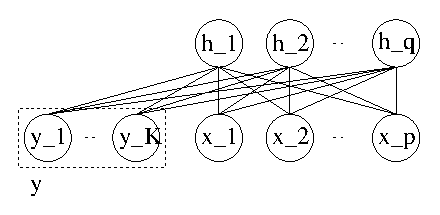
\includegraphics[width=0.9\columnwidth]{figures/drbm.eps}
    \end{minipage}
    \begin{minipage}{0.48\textwidth}
        \centering
        \psfrag{x_1}[Cc][Cc][1][0]{$x_1$}
        \psfrag{x_2}[Cc][Cc][1][0]{$x_2$}
        \psfrag{x_p}[Cc][Cc][1][0]{$x_p$}
        \psfrag{y_1}[Cc][Cc][1][0]{$y_1$}
        \psfrag{y_K}[Cc][Cc][1][0]{$y_K$}
        \psfrag{y}[Cc][Cc][1][0]{$y \in \left\{ 1, \cdots, K\right\}$}
        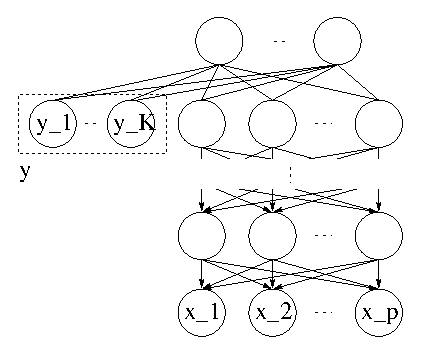
\includegraphics[width=0.9\columnwidth]{figures/ddbn.eps}
    \end{minipage}
    \begin{minipage}{0.48\textwidth}
        \centering
        \small
        (a) Discriminative RBM
    \end{minipage}
    \begin{minipage}{0.48\textwidth}
        \centering
        \small
        (b) Discriminative DBN
    \end{minipage}
    \caption{Illustrations of a discriminative restricted
    Boltzmann machine and discriminative deep belief
    network. Note that the $1$-of-$K$ coding is used for the
    output label $y$ which may take $K$ discrete values.}
    \label{fig:drbm}
\end{figure}

A similar idea was also presented earlier for a deep belief
network (DBN) by \citet{Hinton2006nc}. Instead of augmenting
the visible layer with a transformed label $\vy$, they
augmented the penultimate layer. The augmented units
corresponding to $\vy$ are only connected to the top layer
with undirected edges. See Fig.~\ref{fig:drbm}(b) for
illustration.

This model can be trained by the procedure described in
Section~\ref{sec:dbn}, however with a slight modification.
Firstly, during the first stage of layer-wise pretraining,
we augment the posterior distribution of the penultimate
layer with the labels of the training samples. During the
second stage, where the up-down algorithm is used, the Gibbs
sampling steps between the top two layers start from the
samples from the (approximate) posterior distribution
attached with the labels of the samples in a minibatch. 

Once training is over, we can classify a new sample $\vx^*$
easily by first obtaining the approximate (fully factorized)
posterior means of the penultimate layer $\vmu^*$ and
computing the unnormalized probabilities of the combination
of $\vmu^*$ and all possible label states $\vy$. The one
that gives the largest unnormalized probability is
chosen as a prediction $\hat{\vy}$.

Surprisingly, both of these approaches which perform both
generative $p(\vx, y)$ and discriminative $p(y \mid \vx)$
modeling achieve a classification performance comparable
to or often better than the models which were trained
purely to perform discriminative modeling
\citep{Hinton2006nc,Larochelle2008}.

\subsection{Deep Boltzmann Machine to Initialize an MLP}
\label{sec:mlp_dbm}

It is straightforward to initialize a multi-layer perceptron
(MLP) with a deep belief network (DBN) as well as a
restricted Boltzmann machine (RBM). Once the parameters of
those unsupervised neural networks are estimated, we can
directly use them as initial parameters of an MLP. This
corresponds to the layer-wise pretraining scheme discussed
in Section~\ref{sec:layer_wise_pretraining}.  However, when
it comes to a deep Boltzmann machine (DBM), one must take
into account the nature of each layer receiving both
bottom-up and top-down signals.

A naive way of utilizing a DBM for a discriminative task in
this case is to forget about transforming it into an MLP,
and simply use the approximate posterior means of hidden
units as features (see, e.g., \citet{Montavon2012ai} and
\citepub{Cho2013icann}). In other words, for
each sample $\vx$ we compute the variational parameters
$\vmu$ by maximizing the variational lower bound in
Eq.~\eqref{eq:dbm_lowerbound} with respect to them. Then
the obtained variational parameters are used instead of the
original sample.  However, it is often obvious that a
better discriminative performance is achieved when the model
is specifically \textit{finetuned} to optimize it.

\citet{Salakhutdinov2009a} proposed that the structure of an
MLP be modified to simulate the top-down signal in a DBM.
Given a DBM with $L$ hidden layers
$\left\{\vh^{\qlay{l}}\right\}_{l=1}^L$ and a single visible
layer $\vx$, let us construct an MLP with $L$ intermediate
hidden layers
$\left\{\tilde{\vh}^{\qlay{l}}\right\}_{l=1}^L$, 
a single output layer $\tilde{\vy}$ and a single visible
layer $\tilde{\vx}$.
The main goal of this construction is to make sure that a
single forward pass results in the states of the units in
the penultimate layer $\vh^{\qlay{L}}$ of the MLP being identical
to the mean-field approximation $\vmu^{\qlay{L}}$ of them. 

The fixed point of the variational parameters of the first
hidden layer that locally maximizes the variational
lower bound in Eq.~\eqref{eq:dbm_lowerbound} is
\[
\vmu^{\qlay{1}} = \phi\left( \mW^\top \vx + \mU^{\qlay{1}} \vmu^{\qlay{2}} \right),
\]
where $\phi$ is a component-wise logistic sigmoid function.
Then, if we let the visible layer of the MLP to be
$\tilde{\vx} = \left[ \vx^\top, {\vmu^{\qlay{2}}}^\top
\right]^\top$ and connect $\vx$ with the first hidden layer
of the MLP by $\mW$ and $\vmu^{\qlay{2}}$ by ${\mU^{\qlay{1}}}^\top$,
a single forward pass will result in the activation of the
first hidden layer of the MLP $\tilde{\vh}^{\qlay{1}}$ to be
exactly $\vmu^{\qlay{1}}$.

This applies similarly to all intermediate hidden layers of
the DBM. For any $l$-th layer of the DBM, where $l < L - 1$,
we constrain the $l$-th hidden layer of the MLP by appending
%$\vmu^{\qlay{l}}$ 
$\tilde{\vh}^{\qlay{l}}$ 
with $\vmu^{\qlay{l+2}}$. By connecting them to
$\tilde{\vh}^{\qlay{l+1}}$ with the corresponding weights from
the DBM, we can ensure that the activation of the $(l+1)$-th
hidden layer of the MLP will be initially identical to
$\vmu^{\qlay{l+1}}$. 

Since the last hidden layer of the DBM only receives the
bottom-up signal, there will be no need to construct the
last hidden layer in this way. 
Simply it is 
enough to connect $\tilde{\vh}^{\qlay{L}}$ with
$\tilde{\vh}^{\qlay{L-1}}$ by $\mU^{\qlay{L-1}}$.

\begin{figure}[t]
    \centering
    \psfrag{x}[Bc][Bc][1][0]{$\vx$}
    \psfrag{h1}[Bc][Bc][1][0]{$\vh^{\qlay{1}}$}
    \psfrag{h2}[Bc][Bc][1][0]{$\vh^{\qlay{2}}$}
    \psfrag{Q2}[Bc][Bc][1][0]{$\vmu^{\qlay{2}}$}
    \psfrag{W}[Cc][Cr][1][0]{$\mW$}
    \psfrag{U}[Cl][Cr][1][0]{$\mU$}
    \psfrag{Ut}[Bc][Bc][1][0]{$\mU^\top$}
    \psfrag{y}[Bc][Bc][1][0]{$\vy$}
    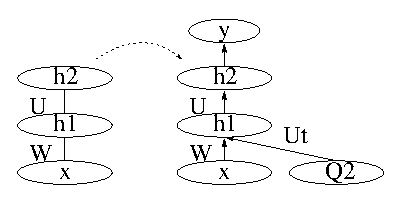
\includegraphics[width=0.75\columnwidth]{figures/dbm_mlp.eps}
    \caption{A deep Boltzmann machine with two hidden
    layers, on the left, is transformed to initialize a
    multi-layer perceptron on the right. $\vmu^{\qlay{2}}$ is a
    vector of the variational parameters of the second
    hidden layer of the DBM.}
    \label{fig:dbm_mlp}
\end{figure}

This way of constructing an MLP (see Fig.~\ref{fig:dbm_mlp})
guarantees that the activation of the last hidden layer of
the MLP after a forward pass with the initialized weights
will coincide with their variational parameters. From there
on, we can use backpropagation (see
Section~\ref{sec:backprop}) to further finetune the model.

For instance, in \citep{Salakhutdinov2009a} and
\citep{Hinton2012}, this way of initializing an MLP with a
DBM was shown to improve the performance on handwritten
digits as well as 3-D object recognition tasks.





\section{Pretraining Generative Models}
\label{sec:pretrain_gen}


So far in this chapter we have described how 
unsupervised neural networks can be used to improve 
performance in supervised tasks. In this section we will
discuss how a simpler unsupervised neural network can help
training more complex, deeper unsupervised neural networks
with some theoretical guarantees.

Earlier in this chapter we have looked at incremental
feature learning from the perspective of an \textit{incremental
transformation} that nonlinearly transforms an input into a
better representation. Once the features are obtained by
the incremental transformation, they are fed to another
machine learning model, or the last pair of layers in an
MLP, to perform a task whose objective was not necessarily
utilized when learning the transformation. However, there is
another perspective from which the incremental
transformation can be viewed.

In Section~\ref{sec:dbn}, we described the learning
algorithm for training a deep belief network (DBN). It is
obvious now to see that the first stage of the learning
algorithm does almost exactly what the incremental feature
learning introduced earlier in this chapter does. Starting
from a single restricted Boltzmann machine (RBM) trained on
original training samples, we repeatedly stack an RBM
trained on the aggregate posterior distribution of the
previous RBM on top.  However, the ultimate goal of this
almost identical procedure was very different.  The goal of
this procedure in training a DBN was to build a good
\textit{generative} model that learns the data distribution
well, rather than to nonlinearly transform the input space
so that another machine learning task will benefit from the
new, better representation.

Ultimately it is a question of what or how much
stacking another restricted Boltzmann machine on top of the
existing deep neural network improves the performance.
Furthermore, one might ask if another pretraining scheme,
other than incrementally stacking shallow models, is
possible.

In the remainder of this section, we first describe how an
RBM can be viewed as an infinitely deep sigmoid belief
network with tied weights \citep{Hinton2006nc}. Based on
this observation we describe in more detail how stacking
RBMs improves the generative performance of a DBN according
to the argument given in
\citep{Hinton2006nc,Salakhutdinov2012nc}.  We then continue
on to discuss how this scheme can be extended to
initializing the parameters of a deep Boltzmann machine
(DBM) based on
\citep{Salakhutdinov2012nc,Salakhutdinov2012}. At the end of
the section, another pretraining scheme for DBMs, proposed in
\citepub{Cho2013icann}, utilizing such directed deep neural
networks as deep autoencoders and DBNs is introduced.


\subsection{Infinitely Deep Sigmoid Belief Network with
Tied Weights}
\label{sec:inf_sbn_rbm}

\begin{wrapfigure}{I}{0.4\textwidth}
%\begin{figure}[t]
    \centering
    \psfrag{x}[Bc][Bc][1][0]{$\vx$}
    \psfrag{h}[Bc][Bc][1][0]{$\vh$}
    \psfrag{x0}[Bc][Bc][1][0]{$\vx^{(0)}$}
    \psfrag{x1}[Bc][Bc][1][0]{$\vx^{(-1)}$}
    \psfrag{x2}[Bc][Bc][1][0]{$\vx^{(-2)}$}
    \psfrag{x3}[Bc][Bc][1][0]{$\vx^{(-3)}$}
    \psfrag{h0}[Bc][Bc][1][0]{$\vh^{(0)}$}
    \psfrag{h1}[Bc][Bc][1][0]{$\vh^{(-1)}$}
    \psfrag{h2}[Bc][Bc][1][0]{$\vh^{(-2)}$}
    \psfrag{W}[Bc][Bc][1][0]{$\mW$}
    \psfrag{Wt}[Bc][Bc][1][0]{$\mW^\top$}
    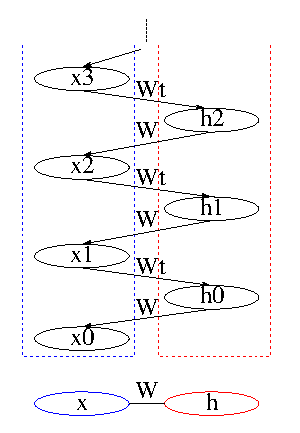
\includegraphics[width=0.4\columnwidth]{figures/rbm_dbn.eps}
    \caption{The ancestral sampling on an infinitely deep
    sigmoid belief network with tied weights is equivalent
    to the block Gibbs sampling on a restricted Boltzmann
    machine.}
    \label{fig:inf_sbn}
%\end{figure}
\end{wrapfigure}

The most straightforward way to obtain samples from a
sigmoid belief network is to sample from the conditional
distribution of each layer given the states of the layer
immediately above, starting from the top layer. An unbiased
sample can be easily obtained from the top layer, since the
prior distribution of the units in the top layer is
factorized. Simply, for each variable in the top layer, we
flip a coin with a probability decided by $\phi(b_i)$
where $b_i$ is the bias and $\phi$ is a logistic sigmoid
function. This way of gathering samples in a directed
network is often known as \textit{ancestral sampling}
\citep[see, e.g.,][]{Bishop2006,Murphy2012}.

Let us construct a sigmoid belief network with infinitely
many layers, given a set of parameters from an RBM. The bottom
layer corresponds to the visible layer of the RBM, and there
are directed edges from the layer above which corresponds to
the hidden layer of the RBM. The weights of the edges are
set to those of the RBM. Again, on top of the second layer,
another layer that corresponds to the visible layer of the
RBM is connected with the downward directed edges whose
weights are fixed to those of the RBM. We repeat this step
infinitely, and we get the infinitely deep sigmoid belief
network with tied weights\footnote{For simplicity, we
omit biases, but they can be considered a part of the
weights.}. 

Let us perform ancestral sampling from a layer, very far up
from the first layer denoted $\vx^{\qlay{-L}}$, in the infinite
limit of $L$ that corresponds
to the visible layer, starting from a random state.  Next,
we will sample from the conditional distribution of a layer
immediately below $\vh^{\qlay{-L}}$ that corresponds to the
hidden layer of the RBM. Subsequently, we will repeatedly
sample from the conditional distributions of $\vx^{\qlay{-L+1}}$,
$\vh^{\qlay{-L+1}}$, $\vh^{\qlay{-L+2}}$, $\vh^{\qlay{-L+2}}$, \dots,
$\vh^{\qlay{-1}}$, and $\vx^{\qlay{0}}$, where $\vx^{\qlay{0}}$ is the
visible layer (See Fig.~\ref{fig:inf_sbn}). 

It is easy to see that this is exactly what Gibbs sampling
does to get samples from the model distribution of an RBM.
If this procedure starts from a layer far enough from the
visible layer, the Gibbs chain will reach the equilibrium
distribution by the time samples from the bottom layers are
collected. 

This means that if, instead of a random state, we perform
the same sampling procedure while fixing all those layers
that correspond to the visible layer of the RBM to a given
sample, the samples of the other layers will represent the
true posterior distribution which is factorized equivalently
to the posterior distribution over the hidden units of the
RBM. In other words, in this infinitely deep sigmoid belief
network, we can sample \textit{exactly} from the posterior
distribution over the hidden units, because the weights are
tied.

\subsection{Deep Belief Network: Replacing a Prior with a
Better Prior}
\label{sec:dbn_rbm}

Here, we take a more detailed look at the first stage of the
learning algorithm of a DBN.
%discussed in Section~\ref{sec:dbn}. 
The first stage consists of
iteratively training an RBM on the samples collected from
the posterior distribution of the hidden units of an RBM
immediately below. Let us first consider a DBN with two
layers of hidden units where the second hidden layer has
as many units as there are visible units.

The first RBM trained on a training set $D$ with $N$ samples
learns
\[
p(\vx \mid \TT_1) = \sum_{\vh^{\qlay{1}}} p(\vh^{\qlay{1}}\mid \TT_1) p(\vx \mid
\vh^{\qlay{1}}, \TT_1),
\]
where $p(\vh^{\qlay{1}}\mid \TT_1)$ is a \textit{prior} distribution
of the hidden units parameterized with $\TT_1$ defined by
\[
p(\vh^{\qlay{1}} \mid \TT_1) = \sum_{\vx} p(\vh^{\qlay{1}}, \vx \mid \TT_1).
\]
We used the superscript $\qlay{1}$ to indicate that the hidden
units are in the first hidden layer of a DBN.

An interesting observation can be made here.  The same set
of parameters $\TT_1$ is used to model both the
conditional distribution $p(\vx \mid \vh^{\qlay{1}})$ and the
prior distribution $p(\vh^{\qlay{1}})$. From this observation, it
is natural to consider \textit{replacing} the prior of
$\vh^{\qlay{1}}$ such that it is not anymore constrained to be
modeled with the same parameters $\TT_1$.
In other words, we would like to replace
$p(\vh^{\qlay{1}} \mid \TT_1)$ with
\[
p(\vh^{\qlay{1}} \mid \TT_2) = \sum_{\vh^{\qlay{2}}}
p(\vh^{\qlay{1}},
\vh^{\qlay{2}} \mid \TT_2).
\]

First, we need to recall that the infinitely deep sigmoid
belief network with \textit{tied} weights is equivalent to
an RBM from Section~\ref{sec:inf_sbn_rbm}. Then, since the DBN
considered here has as many units in $\vh^{\qlay{2}}$ as there
are in the visible layer $\vx$, we get the same model even
after replacing the prior, if we fix $\TT_2$ to
$\TT_1$\footnote{ If we only consider the weights, assuming
that the weights include the biases,
$\mW_{\qlay{2}}=\mW_{\qlay{1}}^\top$.
However, without loss of generality, we simply state that
$\TT_2=\TT_1$.  }.

Let us write the variational lower bound of the marginal
log-likelihood, as described in
Eq.~\eqref{eq:mll_decom}--\eqref{eq:kldiv}, for the DBN with
two hidden layers:
\begin{align}
    \label{eq:dbn_two_layer}
    \sum_{n=1}^N \log p(\vx^{(n)} \mid \TT) &\geq
    \sum_{n=1}^N \left(\E_{Q(\vh^{\qlay{1}} \mid \vx^{(n)})} \left[
    \log p(\vx^{(n)}, \vh^{\qlay{1}} \mid \TT_1)
    \right] + \HH(Q)\right) 
    \nonumber \\
    &= \sum_{n=1}^N \left(\E_{Q(\vh^{\qlay{1}} \mid \vx^{(n)})} \left[
    \log p(\vx^{(n)} \mid \vh^{\qlay{1}}, \TT_1) \right] +
    \HH(Q)\right)
    \nonumber \\
    &\phantom{= \sum_{n=1}^N} + \sum_{n=1}^N
    \E_{Q(\vh^{\qlay{1}} \mid \vx^{(n)})} \left[ \log
    \sum_{\vh^{\qlay{2}}} p(\vh^{\qlay{1}}, \vh^{\qlay{2}} \mid \TT_2) \right]
    ,
\end{align}
where $\HH(Q)$ is the entropy functional of $Q$. This bound
holds for any $Q(\vh^{\qlay{1}} \mid \vx)$, but when $\TT_1 =
\TT_2$, we can use the true posterior $p(\vh^{\qlay{1}} \mid
\vx)$ to make the bound equal to the marginal
log-likelihood.

In Eq.~\eqref{eq:dbn_two_layer}, we can see that only the
last term is dependent on $\TT_2$. This means that if we
increase the last term which corresponds to training another
RBM on the aggregate posterior\footnote{The aggregate
posterior was described in Section~\ref{sec:dbn} as a
mixture of $N$ posterior distributions.} by using the
stochastic approximation method, we can improve the bound,
ignoring any possible stochastic fluctuation. 
This, however, will move $Q$ away from the true posterior
distribution, as $\TT_2$ is now different from $\TT_1$,
which makes the bound less tight.

Once $\TT_2$ is estimated, we can recursively perform this
procedure to replace the prior distribution of
$\vh^{\qlay{2}}$, and so on.  Each replacement will result
in an improved bound, making the generative model possibly
better and better each time.  The approximate posterior
distribution $Q$, however, becomes less and less tight each
time, and the second stage, called the up-down algorithm
\citep{Hinton2006nc}, is needed to jointly estimate both the
recognition and generation parameters of all layers.  

This guarantee of improving the variational lower bound
\textit{only} holds when
\begin{enumerate}
        \vspace{-5mm}
    \itemsep 0em
    \item The weights are initialized to be identical to
        those of the lower layer,
    \item Samples from the aggregate posterior are used, and
    \item RBMs are trained to maximize the log-likelihood.
\end{enumerate}

However, in practice, most of these conditions are violated. The weights
of the newly added RBM are often randomly initialized, and
the probabilities rather than samples of the lower hidden
units are used. Furthermore, in most cases due to the
computational reason, RBMs are trained by minimizing the
contrastive divergence. 

\subsubsection{Stochastic Units vs. Deterministic Units}
\label{sec:det_vs_sto}

Let us discuss slightly more about using probabilities
instead of actual samples as training samples for training
an upper RBM. This can be considered as using a different
approximate posterior distribution $Q$.

In the original proper pretraining procedure, the
approximate posterior distribution
\[
Q(\vh) = \prod_{l=1}^L q_{\vmu^{\qlay{l}}}\left(
\vh^{\qlay{l}} \right)
\]
is defined to be factorized only \textit{layer-wise}. In
other words, the hidden units are not mutually independent
across layers, but only mutually independent inside each
layer given the sampled activations of the units in the
lower layer.

Because of this we obtain the variational parameters
$\vmu^{\qlay{l}}$ iteratively, starting from the first hidden
layer by
\begin{align}
    \label{eq:dbn_posterior}
    \vmu^{\qlay{l}} = \phi\left( \mW_{\qlay{l-1}}^\top
    \tilde{\vh}^{\qlay{l-1}} + \vb_{\qlay{l}} \right),
\end{align}
where $\tilde{\vh}^{\qlay{l-1}}$ is a vector consisting of
elements sampled by 
\[
\tilde{h}_k^{\qlay{l-1}} \sim q\left(h_k^{\qlay{l-1}} = 1 \mid
\mu_k^{\qlay{l-1}}\right).
\]
Here $\phi$ is a sigmoid function as usual. This is
equivalent to performing a feedforward pass on the encoder
of a \textit{stochastic} autoencoder (see
Section~\ref{sec:sbn_dbn}).

We can design another approximate posterior distribution
$\tilde{Q}$ such that the variational parameters
$\vmu^{\qlay{l}}$ are obtained without actual sampling of hidden
units. This new posterior distribution will correspond to
using probability values instead of sampled activations to
train an upper RBM.

Again, the approximate posterior distribution is defined by
\[
\tilde{Q}(\vh) = \prod_{l=1}^L \tilde{q}_{\tilde{\vmu}^{\qlay{l}}}\left(
\vh^{\qlay{l}} \right)
\]
However, in this case we assume a \textit{fully}-factorized
distribution. 

To cope with this assumption, the procedure for computing
the variational parameters $\tilde{\vmu}^{\qlay{l})}$ should
be modified accordingly.  The variational parameters of the
$l$-th layer are now computed recursively using the
following formula: 
\begin{align}
    \label{eq:dbn_posterior_ff}
    \tilde{\vmu}^{\qlay{l}} = \phi\left( \mW_{\qlay{l-1}}^\top
    \tilde{\vmu}^{\qlay{l-1}} + \vb_{\qlay{l}} \right).
\end{align}

One can immediately see that this is equivalent to the
encoder part of a \textit{deterministic} autoencoder.
However, the decoder part still differs from an autoencoder
in the sense that it propagates down sampled activations,
not the real-valued probabilities.  Roughly put, this
difference can be understood so that the decoder of the
autoencoder approximates the generation path of a deep
belief network by using again a fully factorized distribution.
Table~\ref{tbl:dbn_ae} summarizes these differences.

\begin{table}[h]
\vskip 0.15in
    \centering
    \begin{tabular}{c || c | c | c}
        %\multicolumn{1}{r}{Exact}&
        %\multicolumn{2}{c}{$\xrightarrow{\hspace{6.5cm}}$} 
        %& \multicolumn{1}{l}{Approximate} \\
        & DBN & DBN-FF & AE \\
        \hline
        \hline
        Recognition & Layer-wise Factorial & Fully Factorial & Fully Factorial \\
        \hline
        Generation & Layer-wise Factorial & Layer-wise Factorial & Fully Factorial \\
    \end{tabular}
    \caption{The forms of approximate/exact 
    distributions used by a deep belief network (DBN), a
    deep belief network pretrained by a stack of RBMs with
    probabilities used for training upper RBMs (DBN-FF), and
    a deep autoencoder (DAE).}
    \label{tbl:dbn_ae}
\end{table}


The latter choice of an approximate posterior distribution
has two obvious advantages. Firstly, the computation is
easier, since no sampling is required. Also, the
approximated variational parameters are less noisy, since no
stochastic mechanism is involved. However, this choice
nullifies the guarantee discussed earlier in
Section~\ref{sec:dbn_rbm}.

Based on this and the similarity between the fully
factorized approximate posterior and the encoder of a
deterministic autoencoder, we informally conclude that in
terms of generative modeling of data, autoencoders may lag
behind a deep belief network of the same structure. However,
in practice where features extracted by these models are
more interesting, the fully factorized approximate posterior
is often used to train even a deep belief network.
Furthermore, since the network can be further finetuned
generatively by the up-down algorithm (see
Section~\ref{sec:dbn}) later on, the importance of using a
layer-wise factorized approximate posterior distribution
using pretraining diminishes.



\subsection{Deep Boltzmann Machine}
\label{sec:dbm_pre}

In the paper where a deep
Boltzmann machine was proposed, \citet{Salakhutdinov2009a} noticed that it is difficult
to estimate the parameters well. Hence, they proposed a
layer-wise pretraining scheme for deep Boltzmann machines
that facilitates estimating its parameters
\citep{Salakhutdinov2012nc}. The proposed layer-wise
pretraining scheme was further improved in
\citep{Salakhutdinov2012} to better utilize the undirected
nature of the connectivity in a deep Boltzmann machine.

Firstly, we must realize that all the edges in a DBM are
\textit{undirected}. This is a critical difference with a
DBN, when we consider the conditional distribution of a
single intermediate hidden layer $\vh^{\qlay{l}}$. In a DBN, this
is simply conditioned on the layer immediately above
$\vh^{\qlay{l+1}}$, whereas the conditional distribution under a
DBM is conditioned on both the layers immediately
\textit{above} and \textit{below} such that
\[
p(h^{\qlay{l}}_j = 1 \mid \vh^{\qlay{l-1}}, \vh^{\qlay{l+1}}, \TT) = \phi\left(
\sum_{k=1}^{q_{l-1}} h^{\qlay{l-1}}_k w_{kj}^{\qlay{l-1}} +
\sum_{i=1}^{q_{l+1}} h^{\qlay{l+1}}_i w_{ji}^{\qlay{l}} +
c_j^{\qlay{l}}
\right),
\]
where we follow the notations from Section~\ref{sec:dbm}.

Simply put, DBMs must be pretrained while taking into
account that each hidden unit receives a signal from both
upper and lower layers. On the other hand, no such
considerations are needed when pretraining a DBN. If the same
pretraining method for DBNs is used, the conditional
distribution of each hidden unit will be too peaked and
saturated to prevent any further finetuning (jointly
optimizing the whole layers) to improve the model.

\citet{Salakhutdinov2009a} proposed to modify the
structure of RBMs to cope with this difference. For the
bottom two layers, an RBM is modified to have two copies of
visible units with tied weights such that the
additional set of visible units supplies signal that
compensates for the lack of signal from the second hidden
layer. Similarly, an RBM that consists of the top two layers
has the two copies of hidden units. For any pair of intermediate
hidden layers, an RBM is constructed to have two copies of
both visible and hidden units. See Fig.~\ref{fig:dbm_pre}
for an illustration.

\begin{figure}[t]
    \centering
    \psfrag{x}[Bc][Bc][1][0]{$\vx$}
    \psfrag{h1}[Bc][Bc][1][0]{$\vh^{\qlay{1}}$}
    \psfrag{h2}[Bc][Bc][1][0]{$\vh^{\qlay{2}}$}
    \psfrag{h3}[Bc][Bc][1][0]{$\vh^{\qlay{3}}$}
    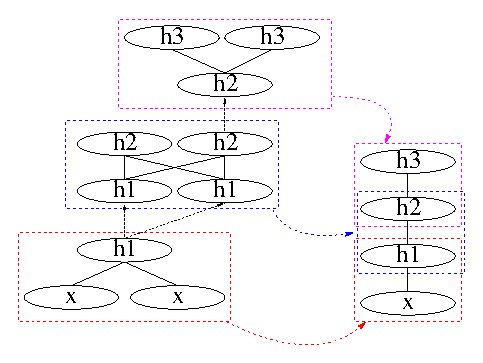
\includegraphics[width=0.73\columnwidth]{figures/pretrain_dbm.eps}
    \caption{Illustration of the layer-wise pretraining of
    a deep Boltzmann machine. The dashed directed lines
    indicate \textit{copying} either the pretrained models or
    the activations of the hidden units of the pretrained
    models.}
    \label{fig:dbm_pre}
\end{figure}

Recently, \citet{Salakhutdinov2012nc} were able to show that
the variational lower bound is guaranteed to increase by
adding the top hidden layer using the proposed pretraining
scheme. Although their proof only applies to the top layer,
it is worth discussing it in relation to the pretraining
scheme for DBNs.

We can rewrite the variational lower bound of a 
DBN 
%having two hidden layers
given in
Eq.~\eqref{eq:dbn_two_layer} as
\begin{align}
    \label{eq:dbn_two_layer2}
    \sum_{n=1}^N \log p(\vx^{(n)} \mid \TT) 
    &\geq 
    \sum_{n=1}^N \left(\E_{Q(\vh^{\qlay{1}} \mid \vx^{(n)})} \left[
    \log p(\vx^{(n)} \mid \vh^{\qlay{1}}, \TT_1) \right]
    \right.
    \nonumber \\
    &\phantom{= \sum_{n=1}^N (\E}\left.+\E_{Q(\vh^{\qlay{1}} \mid \vx^{(n)})} \left[ 
    \log \frac{p(\vh^{\qlay{1}} \mid
    \TT_2)}{Q(\vh^{\qlay{1}}\mid\vx^{(n)})}
    \right] \right)
    \nonumber \\
    &=\sum_{n=1}^N 
    \left(\E_{Q(\vh^{\qlay{1}} \mid \vx^{(n)})} \left[
    \log p(\vx^{(n)} \mid \vh^{\qlay{1}}, \TT_1) \right]
    \right.
    \nonumber \\
    &\phantom{=\sum_{n=1}^N (\E}- \left.\KL\left(
    Q(\vh^{\qlay{1}}\mid\vx^{(n)}) \| p(\vh^{\qlay{1}}\mid
    \TT_2) \right)
    \right).
\end{align}
From this, it is clear that replacing the prior of the first
hidden layer to improve the lower bound is equivalent to
estimating $\TT_2$ such that the new prior distribution
$p(\vh^{\qlay{1}}\mid\TT_2)$ becomes closer to the aggregate
posterior, since the KL-divergence between two distributions
is non-negative and becomes zero only when they are
identical.

If we train the first RBM with two copies of visible
units ($\vx$ and $\vh^{\qlay{2}}$), following the pretraining algorithm of a
\textit{DBM}, we can compute the marginal or prior
distribution over $\vh^{\qlay{1}}$ by using the fact that by
considering $\vh^{\qlay{1}}$ as a visible layer, the whole model
is simply a product-of-expert (PoE) model (see
Section~\ref{sec:poe}) with a hidden layer consisting of
$\vx$ and $\vh^{\qlay{2}}$. Note that we used $\vh^{\qlay{2}}$ to
denote the second copy of the visible units. The prior
distribution of $\vh^{\qlay{1}}$ is then
\begin{align}
    \label{eq:dbm_prior1}
    p(\vh^{\qlay{1}} \mid \TT_1) = \frac{1}{Z(\TT_1)} \left(
    \sum_{\vx} p(\vh^{\qlay{1}}, \vx \mid \TT_1) \right) \left(
    \sum_{\vh^{\qlay{2}}} p(\vh^{\qlay{1}}, \vh^{\qlay{2}} \mid \TT_1)
    \right).
\end{align}

Since both $\vx$ and $\vh^{\qlay{2}}$ are free variables in
Eq.~\eqref{eq:dbm_prior1}, we can improve the variational
lower bound in Eq.~\eqref{eq:dbn_two_layer2} by replacing it
with an RBM having two copies of hidden units with tied
parameters $\TT_2$. If we start by fixing $\TT_2=\TT_1$ and
follow the steepest gradient direction,
%with the stochastic gradient method, 
the KL-divergence between the aggregate
posterior and the new prior distribution will be guaranteed
to decrease, or stay identical at least, which amounts to
improving the lower bound in Eq.~\eqref{eq:dbn_two_layer2}.
The new prior distribution can be similarly written as
\begin{align}
    \label{eq:dbm_prior2}
    p(\vh^{\qlay{1}} \mid \TT_2) = \frac{1}{Z(\TT_2)} \left(
    \sum_{\vx} p(\vh^{\qlay{1}}, \vx \mid \TT_2) \right) \left(
    \sum_{\vh^{\qlay{2}}} p(\vh^{\qlay{1}}, \vh^{\qlay{2}} \mid \TT_2)
    \right).
\end{align}

With these two RBMs, we can form a DBM with two hidden
layers, by replacing the half of the original prior
distribution in Eq.~\eqref{eq:dbm_prior1} with the half of
the new distribution in Eq.~\eqref{eq:dbm_prior2} such that
\begin{align*}
    p(\vh^{\qlay{1}} \mid \TT_1, \TT_2) = \frac{1}{Z(\TT_1,
    \TT_2)} \left(
    \sum_{\vx} p(\vh^{\qlay{1}}, \vx \mid \TT_1) \right) \left(
    \sum_{\vh^{\qlay{2}}} p(\vh^{\qlay{1}}, \vh^{\qlay{2}} \mid \TT_2)
    \right),
\end{align*}
which is guaranteed to have a smaller KL-divergence from the
aggregate posterior $Q(\vh^{\qlay{1}}\mid \vx)$ than
$p(\vh^{\qlay{1}} \mid \TT_1)$ in Eq.~\eqref{eq:dbm_prior2}
\citep[See Appendix of][]{Salakhutdinov2012nc}. 

Hence, adding one more layer on top of an existing RBM is
guaranteed to improve the variational lower bound, if the
proposed pretraining method is used. However, this procedure
does not extend trivially to the intermediate hidden layers.

This mathematical justification suggests that the
pretraining method for a DBM differs from that for a DBN in
that only \textit{half} of a prior distribution is
replaced by the upper layer. Conversely, it states that the
existing layer is still used to model the remaining half of
the prior distribution, whereas in a DBN the lower layer
only concentrated on modeling the conditional generative
distribution given the state of units in the upper layer. 

In fact, this way of justifying the pretraining algorithm
allows to extend the algorithm so that 
modeling of the prior distribution is distributed
\textit{unevenly}. For instance, \citet{Salakhutdinov2012}
proposed to use \textit{three} copies of visible and hidden
units, respectively, when training the bottom and top RBMs.
This is equivalent to replacing two thirds of the prior
distribution by the top RBM. They were able to show that
better generative models could be learned by DBMs with this
approach.

\subsubsection{Two-Stage Pretraining: From Autoencoders To
Deep Boltzmann Machine}

This layer-wise approach is not the only pretraining method
available for DBMs. In \citepub{Cho2013icann}, another
approach that utilizes a deep belief network or a deep
autoencoder is proposed.

Let us look at the variational lower bound of the marginal
probability of $\vx$ under a DBM using a fully factorized
approximate posterior distribution \\
$Q(\vh) = \prod_{l=1}^L
\prod_{j=1}^{q_l} q(h_j^{\qlay{l}})$, where $q(h_j^{\qlay{l}}=1) =
\mu_j^{\qlay{l}}$:
\begin{align}
    \label{eq:dbm_lowerbound}
    \log p(\vx \mid \TT) \geq  -E (\vx, \vmu) + \HH(Q) - \log Z(\TT),
\end{align}
where $\vmu$ is a vector of all variational parameters.

The parameters of a DBM can be estimated by plugging the EM
algorithm (see Section~\ref{sec:ppca}) in the stochastic
approximation procedure (see Section~\ref{sec:sap}). At each
update step, we first perform the E-step of the EM
algorithm, which is equivalent to maximizing
Eq.~\eqref{eq:dbm_lowerbound} with respect to the
variational parameters $\vmu$. Then, with the fixed $\vmu$,
we compute the stochastic gradient and update the
parameters, which corresponds to the M-step.

The gradient of the marginal log-likelihood of a Boltzmann
machine tries to match two distinct distributions. One
distribution is the model distribution characterized by a
mixture of products of visible samples and the corresponding
posterior distributions over hidden units. The other
distribution, the data distribution, is a mixture of
training samples and the corresponding posterior
distribution. The gradient drives the BM by pushing the
model distribution closer to the data distribution.

At the beginning of learning, as parameters were initialized
to have small magnitude, the variational posterior
distribution of hidden units in the deep layers is
effectively \textit{random} in the sense that each hidden unit
is likely to be 0 or 1 with equal probabilities. This leads
to almost zero gradient with respect to the parameters in
the deep layers, since the (variational) posterior
distributions under the both data and model distributions
match already. Then, it is unlikely that the stochastic
gradient method will make the deep hidden layers useful. In
other words, it is likely that the hidden units in upper
layers will stay random even after many updates, which was
noticed in \citepub{Cho2013ijcnn}.
%\citet{Cho2011dlufl}.

Hence, in \citepub{Cho2013icann} it was claimed that it may
be important to have a sensible variational posterior
distribution to start with. To obtain a sensible variational
posterior distribution, the two-stage pretraining algorithm
proposed in the same paper uses a deep directed
neural network, such as a deep belief network or a deep
autoencoder, that has the similar structure as the target
DBM.

This way of \textit{borrowing} an approximate posterior
distribution from another model is informally justified from
the fact that the lower bound in
Eq.~\eqref{eq:dbm_lowerbound} holds for \textit{any}
distribution $Q$. Thus, we can maximize the variational
lower bound by updating the parameters using the stochastic
gradient method, with any fixed $Q$. This amounts to moving
the true posterior distribution to approximately match the
arbitrary approximate posterior distribution.

Once the true posterior distribution is close enough to the
fixed $Q$, the variational lower bound can be further
maximized using the standard EM approach. In other words,
after some updates we can \textit{free} the variational
posterior distribution $Q$ and let it be estimated by
maximizing Eq.~\eqref{eq:dbm_lowerbound} with respect to the
variational parameters $\vmu$.

Since the units $\vh_+$
in the odd-numbered hidden layers can be explicitly summed
out, one only needs to borrow the approximate
posterior distribution only for those units in the
even-numbered hidden layers. This significantly reduces the
computational time required to train a deep, directed neural
network from which the approximate posterior is borrowed.
%, since the number of the hidden layers in that model is
%halved.

Let us rewrite Eq.~\eqref{eq:dbm_lowerbound} to marginalize
out the units in the odd-numbered hidden layers:
\begin{align}
    \label{eq:dbm_lowerbound2}
    \E_{p_D(\vx)} &\left[ \log p(\vx^{(n)} \mid \TT) \right]
    \geq 
    \nonumber \\
    &\E_{p_D(\vx)Q(\vh_- \mid \vx)} \left[ \log \sum_{\vh_+} \exp\left\{ -E
    (\vx^{(n)}, \vh_-, \vh_+)\right\} \right] + \HH(Q) - \log Z(\TT),
\end{align}
where $p_D(\vx)$ is the data distribution which is
approximated by the set of training samples.

It becomes immediately apparent that the first term of the
lower bound in Eq.~\eqref{eq:dbm_lowerbound2} is equivalent
to the marginal log-likelihood of an RBM having visible
units $\left[ \vx, \vh_- \right]$ and hidden units $\vh_+$
with the data distribution $p_D(\vx) Q(\vh_-\mid\vx)$.
Hence, with the fixed $Q$, we can maximize the lower bound
efficiently using all the available techniques, such as
minimizing contrastive divergence (see
Section~\ref{sec:contrastive_divergence}), the enhanced
gradient (see Section~\ref{sec:enhanced_grad}) and advanced
MCMC sampling methods (see
Section~\ref{sec:parallel_tempering}), for training RBMs.
This stage is referred to as the \textit{second} stage in
the two-stage algorithm.

The arbitrary approximate posterior distribution $Q$ is
found in the first stage. For instance, consider having a
deep belief network that has a visible layer corresponding
to $\vx$, and a number of hidden layers corresponding to the
even-numbered hidden layers $\vh_-$ of the DBM. Then we can
perform layer-wise pretraining described earlier in this
chapter, to estimate the \textit{recognition} parameters
that represent the approximate posterior distribution of the
DBN. 

We may also use a deep autoencoder that consists of the
input and output layers corresponding to $\vx$ and two
copies of hidden layers that correspond to $\vh_-$. Once
trained, either with or without a layer-wise pretraining, we
may use its encoder part to approximate the posterior
distribution over the hidden units.

\begin{figure}[t]
    \centering
    \psfrag{x}[Bc][Bc][1][0]{$\vx$}
    \psfrag{y}[Bc][Bc][1][0]{$\tilde{\vx}$}
    \psfrag{h1}[Bc][Bc][1][0]{$\vh^{\qlay{1}}$}
    \psfrag{h2}[Bc][Bc][1][0]{$\vh^{\qlay{2}}$}
    \psfrag{h3}[Bc][Bc][1][0]{$\vh^{\qlay{3}}$}
    \psfrag{h4}[Bc][Bc][1][0]{$\vh^{\qlay{4}}$}
    \psfrag{Deep Autoencoder}[Bc][Bc][1][0]{Stage 1}
    \psfrag{Restricted Boltzmann}[Bc][Bc][1][0]{Stage 2}
    \psfrag{Deep Boltzmann}[Bc][Bc][1][0]{Finetuning}
    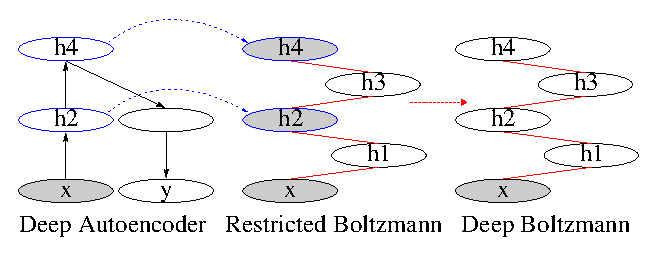
\includegraphics[width=0.85\columnwidth]{figures/pretrain_dbm2.eps}
    \caption{Illustration of the layer-wise pretraining of
    a deep Boltzmann machine. The dashed directed lines
    indicate \textit{copying} of either pretrained models or
    the activations of the hidden units of the pretrained
    models. In this figure, a deep autoencoder is used to
    learn an arbitrary approximate posterior in the first
    stage. The red-colored edges indicate that the weights
    parameters learned in the second stage are used as
    initial values when finetuning the DBM. Note that the
    parameters learned in the first stage are discarded
    immediately after the first stage.}
    \label{fig:two_stage_pretraining}
\end{figure}

In summary, the two-stage algorithm borrows an approximate
posterior distribution from another model trained in the
first stage, and maximizes the variational lower bound with
the variational posterior fixed to the borrowed posterior
distribution\footnote{
We acknowledge here that a similar idea of borrowing an
approximate posterior distribution from another model was
used for a variational Bayesian nonlinear blind source
separation method by \citet{Honkela2004}.
}, as if the DBM were an RBM. See
Fig.~\ref{fig:two_stage_pretraining} for illustration.

This approach was empirically shown to be very effective at
learning a good generative model using a DBM in
\citepub{Cho2013icann}. Furthermore, DBMs with Gaussian
visible units trained using this approach were found to be
good at denoising images corrupted with a high level of noise
%in \citep{Cho2013}.
in \citepub{Cho2013icannA}.













\chapter{Discussion}
\label{chap:discussion}

Lately deep neural networks have shown remarkable
performances in various machine learning tasks. They
include\footnote{For a more comprehensive list, see, for
instance, \citep{Bengio2013pami}.  }, but are not
limited to, speech recognition \citep[see,
e.g.,][]{Hinton2012sp,Dahl2012} and large-scale object
recognition \citep[see, e.g.,][]{Krizhevsky2012,Hinton2012}
as well as natural language processing \citep[see,
e.g.,][]{Socher2011}. In these cases, deep neural networks
were able to outperform the conventional models and
algorithms significantly.

Based on these advances in academic research, deep neural
networks have rapidly found their way into commercial use
through companies such as Google, Microsoft and Apple.  For
instance, Google Goggles\footnote{
http://www.google.fi/mobile/goggles/ } uses a deep belief
network (see Section~\ref{sec:dbn}) in
production\footnote{See the invited talk \textit{Machine
Learning in Google Goggles} by Hartmut Neven at the
International Conference on Machine Learning 2011:
http://techtalks.tv/talks/machine-learning-in-google-goggles/54457/}.
Microsoft has replaced the existing speech recognition
algorithm based on Gaussian mixtures with one based on deep
neural networks \citep{Deng2013}. Furthermore, the voice
assistance feature of Apple's iPhone, called Siri, as well
as Google's Street View are also known to utilize deep
neural networks\footnote{See the article \textit{Scientists
See Promise in Deep-Learning Programs} by John Markoff
featured in the New York Times on 23 November 2012: \\
http://www.nytimes.com/2012/11/24/science/scientists-see-advances-in-deep-learning-a-part-of-artificial-intelligence.html
}.

These recent successes of deep neural networks in both
academic research and commercial applications may be
attributed to several recent breakthroughs. Layer-wise
pretraining of a multi-layer perceptron proposed by
\citep{Hinton2006,Bengio2007nips,Ranzato2007} showed that a
clever way of initializing parameters can easily overcome
the difficulties of optimizing a large, deep neural network.
Furthermore, this new pretraining scheme was found to be a
useful way to incorporate a large amount of unlabeled data
in addition to a small number of labeled data. This led to a
success of deep neural networks, for example, in
unsupervised and transfer learning tasks \citep[see,
e.g.,]{Guyon2011,Mesnil2012,Raina2007}. Beside the
layer-wise pretraining as well as unsupervised learning,
several modifications to multi-layer perceptrons, such as
novel nonlinear hidden units \citep[see,
e.g.,][]{Nair2010,Glorot2011,Goodfellow2013} and dropout
regularization \citep{Hinton2012}, have further pushed the
performance boundary of deep neural networks. 

Despite these recent breakthroughs that brought in the
recent surge of popularity\footnote{As an example of the
increasing popularity of deep neural networks and the field
of deep learning, MIT Technological Review selected deep
learning as one of the ten breakthrough technologies in
2013:
\\http://www.technologyreview.com/featuredstory/513696/deep-learning/
} of deep neural networks, the core principles of building
deep neural networks have evolved rather gradually over more
than 50 years since \citet{Rosenblatt1958} proposed the
perceptron. Over those years many seemingly distant classes
of neural networks as well as other machine learning models
have been proposed and later found to be closely related
\citep[see, e.g.,][]{Haykin2009}. In due course, many
concepts, mainly from probabilistic approaches and
semi-supervised learning, have been absorbed by the field of
neural networks to form the solid basic principles of deep
neural networks.

The main text of this thesis has been written to show how
different perspectives and concepts of machine learning
interact with each other to form the basic principles of deep
neural networks. 

In this last chapter, the author briefly summarizes the main
contents and discusses potential future
research directions. At the end of this chapter, some
important models, concepts as well as practical matters that
have not been discussed in this thesis are briefly
explained.

\section{Summary}

In this thesis, the author has aimed to reveal relationships
among different neural networks as well as other
machine learning methods. Mainly, two classes of deep neural
networks, namely autoencoders and Boltzmann machines, were
discussed in detail and found to be related to each other.
The underlying principles of those two models were found to
be useful in understanding the layer-wise pretraining of a deep
multi-layer perceptron.

The thesis began with simple, linear neural networks.
Linear regression and perceptrons were first described in
terms of neural networks, and later the equivalent models
were formulated from a probabilistic perspective. Similarly, a
linear autoencoder was shown to be equivalent to principal
component analysis as well as its probabilistic variant.

The author went on to describing their deeper, nonlinear
versions which are a multi-layer perceptron in the case of
supervised models, and a deep autoencoder in the case of
unsupervised models. Especially, the thesis focused mainly
on autoencoders. The autoencoder was interpreted as
performing approximate inference and generation in a
probabilistic latent variable model.  Furthermore, the
author explained a geometric interpretation of the states of
hidden units encoded by a variant of autoencoders based on
the manifold assumption which constitutes a central part of
semi-supervised learning.

Independently from autoencoders, the thesis discussed
Boltzmann machines extensively. Starting from Hopfield
networks, which may be seen as a deterministic variant of
Boltzmann machines, the author described in detail
how to estimate the statistics and learn the parameters of Boltzmann
machine as well as their structurally restricted variants
such as the restricted Boltzmann machines (RBM) and the deep
Boltzmann machines. Furthermore, a justification for viewing
Boltzmann machines with hidden units as deep neural networks
was provided in connection to recurrent neural networks.

These two seemingly separate classes of neural networks,
autoencoder and Boltzmann machines, were shown to be closely
related to each other. Especially, an autoencoder with a
single hidden layer was described to be an approximation of
an RBM. The author introduced recent studies showing their
relatedness as well as equivalence. Additionally, a deep
belief network was described as a combination of an RBM and
a deep autoencoder with stochastic units.

At the end of the thesis, the author has explained a recently
introduced method of pretraining a deep multi-layer
perceptron. This method of pretraining, called layer-wise
pretraining, is analyzed from two different viewpoints.
Firstly, the fact that some variants of autoencoders capture
the data manifold was used to view the layer-wise
pretraining as a way of incrementally extracting more useful
features. Secondly, the author explained how stacking
another layer on top of the existing neural network in 
layer-wise pretraining can guarantee the improvement in the
variational lower bound of the marginal log-likelihood.


\section{Deep Neural Networks Beyond Latent Variable Models}

Two different perspectives from which deep neural networks
can be understood have been discussed in this thesis. One is
based on the idea of incrementally capturing the data manifold
through stacking multiple layers of nonlinear hidden units.
The other considers a feedforward computation of a deep
neural network as performing an approximate inference of the
posterior distribution over hidden units in higher layers.

The latter perspective essentially divides a deep neural
network into two distinct parts. The first part is a latent
variable model that models the distribution of training
samples without labels, and then the second part makes a
decision based on the inferred posterior distribution given
a sample, on which class the sample belongs to. For example,
a forward pass computation up until the penultimate layer of
a multi-layer perceptron (MLP, see Section~\ref{sec:mlp})
would correspond to performing an approximate inference, and the
computation from the penultimate layer to the output layer
to decision-making.

In this framework of a latent variable model, the most exact
way of performing classification or decision-making is
to marginalize out hidden variables $\vh$ to obtain the
conditional distribution of missing variables $\vx_m$ given
the states of the observed variables $\vx_o$:
\begin{align*}
    p(\vx_m \mid \vx_o) = \sum_{\vh} p(\vx_m \mid \vh) p(\vh
    \mid \vx_o).
\end{align*}
However, since this exact marginalization is often
computationally intractable, a deep neural network replaces
this with a parametric nonlinear function that computes
\begin{align*}
   % p(\vx_m \mid \vx_o) \approx  
    \sum_{\vh} p(\vx_m \mid
    \vh) Q(\vh \mid \vx_o) 
    \E_Q\left[p(\vx_m \mid
    \vh \right]
\end{align*}
%$\E_{\tilde{p}}\left[ \vx_m \mid \vx_o \right]$ 
in a single sweep.

Assuming a simple, unimodal distribution $p(\vx_m \mid
\vh)$, one consequence of this approximation is that the
approximate predictive distribution $\tilde{p}(\vx_m \mid
\vx_o)$ loses most of the information in the true predictive
distribution $p(\vx_m \mid \vx_o)$. It is natural since
$\tilde{p}(\vx_m \mid \vx_o)$ is unimodal, while the true
predictive distribution could have many probabilistic modes.

The inherent limitations of this approximate approach
employed by deep neural networks are obvious\footnote{Note
that the discussion in this section has been highly
motivated and influenced by Section 5 of
\citep{Bengio2013future}.}. There is no guarantee that the
parametric form employed by a deep neural network of an
approximate posterior distribution $Q$ is good enough to
make the above approximation close to the exact
marginalization.  Furthermore, a usual method of fitting the
variational parameters of $Q$ to minimize the
Kullback-Leibler divergence between $Q$ and the true
posterior distribution $p(\vh \mid \vx_o)$ tends to find
only a single mode of the true posterior distribution, but
we usually cannot tell how representative the found mode is.
If the true posterior distribution is highly multi-modal,
this approximation based on an arbitrary mode will be
generally poor.  Lastly, it is not obvious how a deep neural
network can cope with a more flexible setting where the
observed components are not fixed a priori\footnote{In a
classical setting of, for instance, classification, we know
in advance that label components are not going to be
observed but all other components are.}. 

A way has been proposed to overcome each of these
limitations. For instance, one may bypass the problem of
marginalization or approximate inference by directly mapping
from an input $\vx_o$ to the distribution of $\vx_m$ given
$\vx_o$ which may have been learned by another model such as
a restricted Boltzmann machine \citep{Mnih2011}. In this
way, a deep neural network can learn to approximate a true
predictive distribution $p(\vx_m \mid \vx_o)$ without going
through an extra step of approximation in the middle.
However, if the ultimate goal is to make a decision that
maximizes the predictive performance, we still need to be
able to evaluate either approximately or exactly the
multi-modal predictive distribution quickly and well, which
brings us back to one of the limitations of the current
approach based on the approximate inference of hidden
variables.

A Boltzmann machine provides a principled way to overcome
the problem of having to use an approximate inference of the
posterior distribution over hidden variables. Instead of an
variational approximation, one may perform an
(asymptotically) exact inference utilizing Markov chain
Monte Carlo (MCMC) sampling such that
\begin{align*}
    p(\vx_m \mid \vx_o) \approx \frac{1}{T} \sum_{t=1}^T
    p(\vx_m \mid \vh^{\qt{t}}),
\end{align*}
where $\vh^{\qt{t}}$ is the $t$-th sample from $p(\vh \mid
\vx_o)$. In fact, it is natural with a Boltzmann machine to
consider any combination of observed components and missing
components. Therefore this approach is tempting, but as the
size of a model grows and the number of modes in the
predictive distribution increases, it becomes impractical to
use MCMC sampling for making a rapid decision.

Hence, we want to have a radically new neural network that
keeps the best of the two types of deep neural networks
discussed throughout this thesis. A fast and efficient
computation of feedforward neural networks (see
Chapter~\ref{chap:ffnn}) is required for a rapid
decision-making, while most information and structure
contained in a complex multi-modal predictive distribution
must be maintained, just like a Boltzmann machine is able to
learn a multi-modal distribution (see
Chapter~\ref{chap:bm}). To the author's current knowledge,
there is no such neural network at the moment\footnote{
A few recent works are showing some promising directions using
stochastic neural networks \citet[see,
e.g.,][]{Bengio2013gsn,Tang2013}.  }. It is, hence, left for
future research to build such a neural network that combines these
two very different characteristics.

The ultimate goal of deep neural networks and the field of
deep learning will be to build a large deep neural network
that can learn
\begin{align*}
    f(\vx_o\mid \TT) = \argmax_{\vx_m} p(\vx_m \mid \vx_o),
\end{align*}
where $\TT$ denotes a set of parameters, and the indices of
observed and missing components are not fixed a priori. A
deep neural network that computes this function will have to
be powerful and flexible enough to consider all different
possibilities or modes in the predictive distribution in a
single sweep of the network in a feedforward manner.



\section{Matters Which Have Not Been Discussed}
\label{sec:leftovers}

Despite the original intention of describing in much
details the basics of deep neural networks,
some important models and concepts have been left out from
the main text. The author would like to briefly mention
a few of them here, to provide any interested reader with
some references.

The remainder of this section starts by providing a list of
the previous work that relates independent component
analysis as well as general factor analysis to the models
discussed previously.  Additionally, some references that
attempted to make these models deeper are presented.  

The models described so far in this thesis are fairly
powerful in the sense that many of them have the universal
approximator property. In Section~\ref{sec:mlp}, it was
stated that a multi-layer perceptron has the universal
approximator property, but no results about the other models
were presented nor described. Thus, a list of previous
research results which showed and proved the universal approximator
property of the models discussed earlier in this
dissertation is provided.

Subsequently, we discuss how a Boltzmann machine can be
evaluated. Unlike most feedforward neural
networks, the exact computation of the objective function in
training a Boltzmann machine cannot be done tractably. This
is due to both the intractability of the normalization
constant and the difficulty of marginalizing out hidden
units. Hence, the author discusses some approaches that can
approximately evaluate Boltzmann machines.

Throughout this thesis, there was no discussion on selecting
hyper-parameters that are necessary for training a deep
neural network. Section~\ref{sec:hyperopt} briefly describes
a problem of hyper-parameter selection in one particular
setting of pretraining and finetuning a multi-layer
perceptron, and introduces recently proposed
hyper-parameter optimization approaches based on Bayesian
optimization.

This thesis is directed towards deep neural networks, but it must be
reminded that not all models nor research directions have
been covered. For instance, the entire text was written
assuming that all training samples are independent and
identically distributed, ignoring any temporal dependence.
However, a recurrent neural network described in
Section~\ref{sec:rnn_deep} is capable of learning temporal
dependencies between samples.

Furthermore, it was implicitly assumed that a target task is
permutation invariant, meaning that the structure of a deep
neural network is independent from the order of the
components of an input vector. This ensures that the models
discussed in this thesis are generally applicable to any
data without prior knowledge. However, this may not be an
optimal approach especially in a task which exhibits clear
spatial structures among input components. One such case
involves handling images, and at the end of this section we
briefly discuss an approach based on convolutional neural
networks that specifically aims at handling images.

%In this thesis, except for very few, no further discussion
%on regularizing deep neural networks was made, while it has
%been widely acknowledged that it is extremely important to
%properly regularize a deep neural networks. Lastly, despite
%the fact that training these deep neural networks, even the
%most shallow ones such as a restricted Boltzmann machine, is
%difficult, the author did not attempt to explain practical
%matters regarding learning algorithms. 


\subsection{Independent Component Analysis and Factor Analysis}
\label{sec:ica_fa}

One important model which belongs to a family of linear
generative models is independent component analysis
\citep[ICA, see, e.g.,][]{Hyvarinen2001}. This model is closely related to
many models we have discussed.  For instance, ICA formulated
using the information-theoretic approach by \citet{Bell1995}
is equivalent to the maximum likelihood solution of sparse
coding (see Section~\ref{sec:sparse_coding}) in the limit of
no noise, when the numbers of inputs and
sources are same \citep{Olshausen1997}.  Furthermore, by
replacing the orthogonality constraint with the minimal
reconstruction regularization, it was shown by
\citet{Le2011} that a linear autoencoder (see
Section~\ref{sec:linear_autoencoder}) with a
soft-sparsity regularization on hidden activations is
equivalent to ICA. Similarly, an approach that extracts
principal components can be extended to extract independent
components by employing certain nonlinear
activation functions for the hidden units \citep[see,
e.g.,][]{Oja1997,Hyvarinen2001}. ICA is further related
to a restricted Boltzmann machine (see
Section~\ref{sec:rbm}) via an energy-based model proposed by
\citet{Teh2003}.

There have been approaches to extend basic ICA, which
assumes a single layer of sources, or hidden units, to have
more than one hidden layer. For instance,
\citet{Lappalainen2000} proposed a nonlinear generative
model where the visible variables are generated through
multiple layers of nonlinear hidden units starting from the
mutually independent top hidden units, or sources. They
called this model Bayesian nonlinear independent component
analysis. This qualifies as a deep neural network by
satisfying the first two conditions provided in
Section~\ref{sec:deep_conditions}.

When put into a probabilistic framework, most of these
generative models, including principal component analysis,
ICA and sparse coding, with directed edges are special cases
of factor analysis with certain assumptions. Factor analysis
assumes that the observation has been generated from a
number of factors, or hidden units, via a certain mapping.
In basic factor analysis the mapping is
assumed to be linear, and the factors follow Gaussian
distribution \citep[see, e.g.,][Chapter 12.2.4]{Bishop2006}. 

Similarly to ICA, factor analysis has also been extended
into a nonlinear model with potentially \textit{deep}
structure. \citet{Raiko2001} and \citet{Raiko2007}, for instance,
describe a hierarchical nonlinear factor analysis method which
starts from a set of factors at the top and generates
sequentially a layer of stochastic hidden units until the
visible layer of observed variables. This hierarchical model
can be considered as a generalization of the sigmoid belief
network (see Section~\ref{sec:sbn_dbn}) such that hidden
units are not restricted to be binary. A similar model which
replaces binary units of the sigmoid belief network with
Gaussian units with squashing nonlinearity functions 
was proposed by \citet{Frey1999}.

\subsection{Universal Approximator Property}
\label{sec:uap}

In Section~\ref{sec:mlp}, it was mentioned that a
multi-layer perceptron (MLP) with a single hidden layer has
the universal approximator property provided that there are
enough hidden units. %From this result on an MLP, 
It is natural to question whether any other model
discussed in this dissertation has the same property. 

Support vector machines with certain kernel functions have
the universal approximator property \citep{Hammer2003}.
Furthermore, an extreme learning machine was shown to have
the same property \citep{Huang2006tnn}. Deep autoencoders are
obviously universal approximators in the sense that they can
reconstruct any input sample arbitrary well, as each of them
is equivalent to an MLP.

Similarly, universal approximator property can be defined
for unsupervised models. A model has the universal
approximator property if any distribution can be modeled
arbitrary well with respect to a chosen divergence
criterion by the model.

\citet{Roux2008} and \citet{Freund1994}  proved that a
restricted Boltzmann machine (RBM, see
Section~\ref{sec:rbm}) has this property when any binary
distribution is considered. This naturally extends to the
fact that a deep Boltzmann machine (DBM, see
Section~\ref{sec:dbm}) and a fully-connected Boltzmann
machine are both universal approximator, since they are more
general than an RBM.  Later, the same authors in
\citep{Roux2010} showed that a deep belief network (see
Section~\ref{sec:dbn}) has the same property on any binary
distribution with the upper-bound on the number of units in
each hidden layer, albeit requiring exponentially many
hidden layers with respect to the input dimensionality. 

In \citepub{Cho2013ijcnn}, it was shown that an equivalent
DBM with Gaussian visible units (GDBM) can be constructed for any
mixture of Gaussians \citep[MoG, see, e.g.,][]{Bishop2006}.
Since MoG\nomenclature{MoG}{Mixture of Gaussians}s are universal approximators, so are GDBMs.
However, this argument does not apply to RBMs with Gaussian
visible units (GRBM, see Section~\ref{sec:grbm}), since not
all MoGs can be modeled by GRBMs.

\subsection{Evaluating Boltzmann Machines}
\label{sec:eval_bm}

One important reason that makes training a Boltzmann machine
more difficult than, for instance, an autoencoder is that
the exact computation of the cost function is intractable.
This is an obvious consequence from having an intractable
normalization constant in its formulation (see
Eqs.~\eqref{eq:bm_prob}--\eqref{eq:bm_mll}). Also,
except for restricted Boltzmann machines (RBM), it is
intractable to marginalize hidden units.

\citet{Salakhutdinov2008a} proposed to first estimate the
normalization constant using annealed importance sampling
\citep{Neal1998} and then to use the estimated constant for
computing the variational lower bound (see
Eq.~\eqref{eq:bm_lowerbound}) of either training or test
samples. The average of multiple runs of annealed
importance sampling can compute an unbiased estimate of the
normalization constant. Empirical evidence
\citep{Salakhutdinov2008} showed that the variance of the
estimates is sufficiently small even with only a small
number of runs.  Furthermore, the variational lower bound
turned out to be surprisingly tight in the case of deep
Boltzmann machines \citep{Salakhutdinov2012nc}.

Based on the idea of the annealed importance sampling and
parallel tempering (see
Section~\ref{sec:parallel_tempering}),
\citet{Desjardins2011} introduced a method of tracking the
normalization constant while training a restricted Boltzmann
machine. Also, in \citepub{Cho2011icml} and
\citepub{Cho2013ijcnn} an adaptive learning rate which
estimates the local change in the log-likelihood, or its
variational lower bound up to the constant multiplicative
factor, was
proposed based on the idea of the annealed importance
sampling.

In the case of RBMs, a crude approximation of the cost
function can be computed based on the connection between the
RBM and the autoencoder. Especially, when the RBM is trained
by minimizing the contrastive divergence (see
Section~\ref{sec:contrastive_divergence}), the
reconstruction error (see Section~\ref{sec:cd_rerr}) may be
used to monitor the learning progress \citep{Hinton2012rbm}.
However, as pointed out in \citep{Hinton2012rbm}, the
reconstruction error is \textit{not} an absolute measure of
the performance of an RBM.

\subsection{Hyper-Parameter Optimization}
\label{sec:hyperopt}

One might have noticed throughout this thesis that there are
many hyper-parameters involved in training these deep
neural networks. Typically, training an unsupervised neural
network with a single hidden layer involves, for instance
in the case of a denoising autoencoder, nine
hyper-parameters:
\begin{enumerate}
    \itemsep 0em
    \item The number of hidden units
    \item Noise variance
    \item Drop ratio
    \item Initial learning rate
    \item Learning rate scheduling
    \item Momentum
    \item Weight decay constant
    \item Target sparsity
    \item Sparsity regularization constant
\end{enumerate}
Hence, if we use a denoising autoencoder to pretrain a deep
multi-layer perceptron (MLP), this number of 
hyper-parameters is multiplied by the number of hidden layers
in the MLP. Furthermore, there are 6 more hyper-parameters
that need to be further tuned for finetuning by
backpropagation:
\begin{enumerate}
    \itemsep 0em
    \item Noise variance
    \item Drop ratio
    \item Initial learning rate
    \item Learning rate scheduling
    \item Momentum
    \item Weight-decay
\end{enumerate}
In total, if we have to train a deep MLP using layer-wise
pretraining by denoising autoencoders, we need to choose $9L
+ 6$ hyper-parameters correctly. 

When the number of hyper-parameters is low, it is usual to
use the grid-search to find the best configuration. It is, however,
less preferable in the case of deep neural networks, since
the number of candidate points on the grid grows
exponentially with respect to the number of
hyper-parameters,
which grows linearly with respect to the number of hidden
layers. 

This is highly problematic considering that training even a
single deep neural network is computationally expensive. One
cannot allow training exponentially many deep neural
networks only for selecting the hyper-parameters.
Hence, a hyper-parameter optimization method for deep neural
networks must be able to find only a \textit{small} set of
\textit{good} candidate points in the hyper-parameter space.

Based on this motivation, two recent studies
\citep{Bergstra2011,Snoek2012} explored the idea of using
Bayesian optimization \citep[see, e.g.,][]{Brochu2010}.
Bayesian optimization simultaneously models the posterior
distribution over a function $h(\Psi)$ that maps from a set
$\Psi$ of hyper-parameters to the performance of a model
trained using $\Psi$ and explores the state-space of $\Psi$
to find the maximum of the unknown function $h$.

As both of these approaches have shown promising empirical
result, we finish this section by recommending any of these
two approaches for choosing hyper-parameters of deep neural
networks. We do not go any further into the details of these
algorithms as it is out of the scope of this thesis.

\subsection{Exploiting Spatial Structure: Local Receptive
Fields}
\label{sec:basic_blocks2}

%However, this is not the only way to extract features
%incrementally. Especially, 
When we have prior knowledge about the structure of the
data, it may be possible to exploit it to obtain a better
representation. For instance, a two-dimensional image has a
local structure that is not maintained once the pixels in
the image are shuffled.  Similarly, a segment of speech has
a temporal structure that easily breaks down when the speech
samples are shuffled across time.

In \citep{Coates2011}, an image classification framework
based on a single level of incremental feature learning was
described in detail. The framework consists of three stages;
(1) training a shallow neural network on randomly selected
small image patches from training images, (2) extracting
features from each image using the trained neural network,
and (3) training a (linear) classifier on the extracted
features.  The first two stages correspond to a single step
of the already described incremental feature learning.

The underlying idea in the first two stages is based on 
convolutional neural networks \citep[see,
e.g.,][]{Lecun1998,Lee2009} where a hidden unit is connected
only to a small neighborhood, or local patch, in the input
image. A set of hidden units is trained on a large set of
fixed-size patches of training images, rather than the whole
images.  Then, each image is \textit{scanned} with the
trained neural network to extract features. Each hidden unit
of the model used in this stage is often referred to as a
\textit{local receptive field}.  Usually after this stage
the sets of features from nearby patches are \textit{pooled}
to form a subsampled set of features.

\citet{Coates2011} empirically compared using different
neural networks for the first two stages. They compared
sparse autoencoders (see Section~\ref{sec:spaenc}),
restricted Boltzmann machines with sparsity
regularization, K-means clustering and Gaussian mixtures. In
most cases they considered, they were able to achieve the
state-of-the-art performance.

This approach of convolution and pooling can be further used
as a single stage in incremental feature learning.  In
fact, if we had started our discussion on incremental
feature learning from the convolutional neural
network \citep[see, e.g.,][]{Lecun1998} rather than from the
fully-connected MLP, we would have arrived at the idea of
incremental feature learning where each stage consists of
\textit{convolution}, \textit{contrast normaliziation}, and
\textit{pooling} \citep[see, e.g.,][]{Lecun2010}. \citet{Lee2009} showed that this way of
incrementally stacking convolutional layers enables the
neural network, specifically a convolutional deep belief
network in their work, to learn hierarchical part-based
representations of data.

As the aim of this thesis, however, was not on the specific
tasks of image or audio recognition, which are known to
benefit heavily from this convolutional structure, we have
not discussed it any further. For more details on learning
local receptive fields and using them for image
classification, we refer readers to \citep{Coates2012t}. We
further suggest \citep{Krizhevsky2012} and
\citep{Ciresan2012b} for the latest advances in using
convolutional neural networks for image classification.



\bibliographystyle{abbrvnat}
%\small
\bibliography{dissertation}

%% Examples of article references, remove these from your manuscript!
% Uncomment them, if you want to see the results of these commands in this example document

% % Refer to the Journal paper 1 of this example document
%\citepub{j1} \& \cpub{j1} \& \cp{j1} \& \pageref{j1} \& \ref{j1}

%% Refer to the Conference paper of this example document
%\citepub[p.~2]{c1} \& \cpub[Sec.~ 1]{c1} \&  \cp[pp.~1--2]{c1} \& \pageref{c1} \& \ref{c1} 


% Errata list, if you have errors in the publications.
%\errata

% Set the publication information.
% This command musts to be the first!
\addpublication{Kyunghyun Cho, Tapani Raiko and Alexander
Ilin}{Enhanced Gradient for Training Restricted Boltzmann
Machines}{Neural Computation}{Volume 25 Issue 3 Pages
805--831}{March}{2013}{Massachusetts Institute of Technology}{Cho2013nc}
% Add the errata of the publication, remove if there are
% none (the order can be interchanged with
% \addauthorscontribution).
%\adderrata{This is wrong}
% Add the publication pdf file, the filename is the
% parameter (must be the last).
\addpublicationpdf[scale=1.3,offset=0 0]{papers/Cho2013nc.pdf}

% Set the publication information.
\def\reprintname{}
\addpublication[conference]{Kyunghyun Cho, Tapani Raiko and
Alexander Ilin}{Enhanced Gradient and Adaptive Learning Rate
for Training Restricted Boltzmann Machines}{Proceedings of
the 28th International Conference on Machine Learning (ICML 2011)}
{pages 105--112}
{June}{2011}{The authors}{Cho2011icml}
% No errata
% Add the publication pdf file, the filename is the parameter.
\addpublicationpdf{papers/Cho2011icml.pdf}

\def\reprintname{Reprinted with permission.}
% Set the publication information.
\addpublication[conference]{Kyunghyun Cho, Tapani Raiko and
Alexander Ilin}{Parallel Tempering is Efficient for Learning
Restricted Boltzmann Machines}{Proceedings of the 2010 International Joint
Conference on Neural Networks (IJCNN
2010)}{pages 1--8}{July}{2010}{IEEE}{Cho2010ijcnn}
% No errata
% Add the publication pdf file, the filename is the parameter.
\addpublicationpdf{papers/Cho2010ijcnn.pdf}

\def\reprintname{Reprinted with kind permission of Springer
Science+Business Media.}
% Set the publication information.
\addpublication[conference]{Kyunghyun Cho,
Alexander Ilin and Tapani Raiko}{Tikhonov-Type
Regularization for Restricted Boltzmann
Machines}{Proceedings of the 22nd International
Conference on Artificial Neural Networks (ICANN
2012)}{pages 81--88}{September}{2012}{Springer Science+Business Media}{Cho2012icann}
% No errata
% Add the publication pdf file, the filename is the parameter.
\addpublicationpdf[scale=1.3,offset=0 -10]{papers/Cho2012icann.pdf}

% Set the publication information.
\addpublication[conference]{Kyunghyun Cho,
Alexander Ilin and Tapani Raiko}{Improved Learning of
Gaussian-Bernoulli Restricted Boltzmann
Machines}{Proceedings of the 21st International
Conference on Artificial Neural Networks (ICANN
2011)}{pages 10--17}{June}{2011}{Springer Science+Business
Media}{Cho2011icann}
% No errata
% Add the publication pdf file, the filename is the parameter.
\addpublicationpdf[scale=1.3,offset=0 -35]{papers/Cho2011icann.pdf}

\def\reprintname{Reprinted with permission.}
% Set the publication information.
\addpublication[conference]{Kyunghyun Cho,
Tapani Raiko and Alexander Ilin}{Gaussian-Bernoulli Deep
Boltzmann Machines}{Proceedings of the 2013 International Joint Conference on Neural
Networks (IJCNN 2013)}{}{August}{2013}{IEEE}{Cho2013ijcnn}
% No errata
% Add the publication pdf file, the filename is the parameter.
\addpublicationpdf{papers/Cho2013ijcnn.pdf}

% Set the publication information.
\def\reprintname{Reprinted with kind permission of Springer
Science+Business Media.}
\addpublication[conference]{Kyunghyun Cho, Tapani
Raiko, Alexander Ilin and Juha Karhunen}{A Two-Stage
Pretraining Algorithm for Deep Boltzmann
Machines}{Proceedings of the 23rd International Conference
on Artificial Neural Networks (ICANN
2013)}{}{September}{2013}{Springer Science+Business Media}{Cho2013icann}
% No errata
% Add the publication pdf file, the filename is the parameter.
\addpublicationpdf[scale=1.3,offset=0 -35]{papers/Cho2013icann.pdf}

\def\reprintname{}
% Set the publication information.
\addpublication[conference]{Kyunghyun Cho}{Simple
Sparsification Improves Sparse Denoising Autoencoders in
Denoising Highly Corrupted Images}{Proceedings of the 30th International
Conference on Machine Learning (ICML
2013)}{432--440}{June}{2013}{The authors}{Cho2013icml}
% No errata
% Add the publication pdf file, the filename is the parameter.
\addpublicationpdf{papers/Cho2013icml.pdf}

% Set the publication information.
\def\reprintname{Reprinted with kind permission of Springer
Science+Business Media.}
\addpublication[conference]{Kyunghyun Cho}{Boltzmann
Machines for Image Denoising}{Proceedings of the 23rd International Conference
on Artificial Neural Networks (ICANN
2013)}{}{September}{2013}{Springer Science+Business
Media}{Cho2013icannA}
% No errata
% Add the publication pdf file, the filename is the parameter.
\addpublicationpdf[scale=1.3,offset=0 -35]{papers/Cho2013iclr.pdf}

\def\reprintname{Reprinted with permission.}
% Set the publication information.
\addpublication[conference]{Sami Keronen, Kyunghyun
Cho, Tapani Raiko, Alexander Ilin and Kalle
Palom\"aki}{Gaussian-Bernoulli Restricted Boltzmann
Machines and Automatic Feature Extraction for Noise Robust
Missing Data Mask Estimation}{Proceedings of the 38th International Conference on
Acoustics, Speech, and Signal Processing (ICASSP
2013)}{}{May}{2013}{IEEE}{Cho2013icassp}
% No errata
% Add the publication pdf file, the filename is the parameter.
\addpublicationpdf{papers/Cho2013icassp.pdf}

%% Set the publication information.
%\addpublication[conference,submitted]{Kyunghyun
%Cho}{Boltzmann Machines and Denoising Autoencoders in Image
%Denoising}{International
%Conference on Artificial Neural Networks}{Sofia, Bulgaria}{September}{2013}{Copyright
%Holder}{Cho2013icannA}
%% Add the dissertation author's contribution to that publication.
%\addcontribution{The author did also this and that}
%% No errata
%% Add the publication pdf file, the filename is the parameter.
%%\addpublicationpdf{papers/Cho2013iclr.pdf}



\end{document}
